\pdfoutput=1
\documentclass[aps,prx,twocolumn,superscriptaddress,nofootinbib,longbibliography]{revtex4-2}
\usepackage{amsmath,amssymb,amsthm,mathtools}
\usepackage{graphicx,booktabs}
\usepackage{xcolor}
\usepackage{xr-hyper}
\usepackage[colorlinks=true,linkcolor=blue,citecolor=blue,urlcolor=blue]{hyperref}
% References to the Supplemental Material (supplement.tex) carry the prefix S:; compile
% main.tex, supplement.tex, main.tex.
\externaldocument[S:]{supplement}
% The bibliography is a thebibliography environment in this file (and nofootinbib puts no notes
% into it), so stop REVTeX from reading a main.bbl at its end.
\makeatletter\let\auto@bib@innerbib\@empty\makeatother

\theoremstyle{plain}
\newtheorem{theorem}{Theorem}
\newtheorem{lemma}{Lemma}
\newtheorem{corollary}{Corollary}
\newtheorem{proposition}{Proposition}
\newtheorem{conjecture}{Conjecture}
\theoremstyle{definition}
\newtheorem{definition}{Definition}
\theoremstyle{remark}
\newtheorem{remark}{Remark}

\newcommand{\dproj}{d_{\mathrm{proj}}}
\newcommand{\Tpre}{T_{\mathrm{pre}}}
\newcommand{\Tout}{T_{\mathrm{out}}}
\newcommand{\E}{\mathbb{E}}
\newcommand{\Z}{\mathbb{Z}}
\newcommand{\Q}{\mathbb{Q}}
\newcommand{\R}{\mathbb{R}}
\newcommand{\F}{\mathbb{F}}
\newcommand{\PU}{\mathrm{PU}(2)}
\newcommand{\SU}{\mathrm{SU}(2)}
\newcommand{\tr}{\operatorname{tr}}
\newcommand{\supp}{\operatorname{supp}}
\DeclareMathOperator{\spec}{spec}

\begin{document}

\title{A Memory--Magic Exchange Law in Streaming \texorpdfstring{Clifford+$T$}{Clifford+T} Compilation}

\author{Jinze Yang}
\affiliation{School of Physics, Xidian University, Xi'an 710071, China}

\author{Haotong Luan}
\affiliation{Future Technology School, Shenzhen Technology University, Shenzhen 518118, China}

\author{Yangyang Li}
\email{yyli@xidian.edu.cn}
\affiliation{Key Laboratory of Intelligent Perception and Image Understanding of Ministry of Education of China,
Collaborative Innovation Center of Quantum Information of Shaanxi Province, Institute of Interdisciplinary Quantum Science and Technology (IIQST),
School of Artificial Intelligence, Xidian University, Xi'an 710071, China}

\author{Xiu-Hao Deng}
\email{dengxiuhao@iqasz.cn}
\affiliation{Shenzhen International Quantum Academy, Shenzhen 518048, China}
\affiliation{Shenzhen Branch, Hefei National Laboratory, Shenzhen, 518048, China}

\begin{abstract}
A phase that reaches a fault-tolerant processor in several additive pieces can be remembered until the last piece arrives, or executed on arrival: the first option is paid for in classical bits carried across a round boundary, the second in magic states committed before the phase is known. We show that in the ancilla-free coordinatewise Clifford+$T$ model realized by per-rotation synthesis pipelines the two payments are convertible at an exchange rate $\alpha$---committed $T$ gates per bit of memory forgone---that does not depend on the problem size, and we prove two unconditional bounds on it as $L:=\log_2(1/\varepsilon)\to\infty$. For every process in the model, $\alpha\ge\tfrac52-o(1)$. For rotation-segmented processes, whose every committed piece is within $\varepsilon$ of a Clifford-framed $z$-rotation as in per-rotation pipelines, $\alpha\ge3-o(1)$, and this is the rate: a fractional passthrough family attains $\alpha\to3$ whenever single-rotation synthesis on the grid costs $(3+o(1))L$ on average, as Ross--Selinger synthesis gives for typical angles. Both bounds hold unchanged when the phases cancel and the final unitary is the identity. The proofs count Clifford+$T$ words near rotation cosets: a spectral estimate resting on the Ramanujan bound gives $\alpha\ge2$ with explicit constants, an elementary determinant method crosses its square-root barrier and reaches every $\alpha<\tfrac52$, and a volume law at Clifford-framed cosets gives the rotation-segmented bound. Under an equidistribution conjecture that exhaustive enumeration to $T$-count $22$ supports, $\alpha=3$ for every process and commitment is quantized in whole rotations. At $\varepsilon=10^{-10}$ the rigorous floor is $0.78$ committed $T$ gates per bit against $3.20$ achieved. Probabilistic mixing halves the law without removing it, and clean ancillas with a catalytic phase-gradient register remove it by batching many coordinates: the constant-rate law is specific to coordinatewise synthesis.
\end{abstract}

\maketitle

\section{Introduction}


Two physical resources meet at the boundary between a fault-tolerant quantum processor and its classical control electronics. On the quantum side, every non-Clifford rotation consumes magic states, and the number of $T$ gates is the dominant cost of a logical computation~\cite{BravyiKitaev,Litinski}. On the classical side, an instruction that has been lowered into the pulse stream cannot be taken back, so the only quantity that a round of the computation can pass to the next one is the state it has decided, in advance, to carry~\cite{Caune,Fowler}. These are different resources with different exchange rates against everything else, and there is no a priori reason for them to be convertible into one another.

They become convertible when a phase arrives in pieces. A Trotter step, a randomized-compiling instance, a layerwise parametrized ansatz, or a phase-polynomial emitted by a scheduler presents the angle of a given rotation as a sum of shares delivered in different rounds. Whoever executes the stream then faces a choice at every share: hold it in classical memory until the sum is known and synthesize one rotation, or synthesize the share on arrival and consume the corresponding magic now. Our earlier work~\cite{Paper1} established that the first option is charged in bits: any streaming process that is correct to projective error $\varepsilon$ on all $r$-round dispersed streams of $m$ commuting phases must carry, across the last inter-round cut, $\Omega(m\log(1/\varepsilon))$ bits of restart state or of committed output. The second option was there only estimated, through an empirical synthesis cost of about $3\log_2(1/\varepsilon)$ $T$ gates per rotation. The purpose of this paper is to make the second option a theorem and to determine the exchange rate.

The quantity traded against magic is not storage. A control processor has gigabytes of memory, and at $m=10^4$ coordinates and $\log_2K=33$ the entire aggregate is $41$\,kB, against $10^6$ magic states on the other side of the trade. What the snapshot $S$ below measures is \emph{deferred decision}: how much of the computation a schedule has refused to lower into the instruction stream until later rounds have been seen. Deferral is not free when the stream is append-only and the scheduler emits with bounded lookahead, as in a real-time control stack~\cite{Caune,Fowler}, or when the shares are produced by agents whose randomness the compiler does not hold, as in randomized compiling. The cost of not deferring is a property of the commitment and not of the target: every lower bound below holds conditionally on any fixed aggregate, including the zero aggregate whose target unitary is the identity (Corollary~\ref{cor:identity})---a computation that cancels completely can still have consumed $\Theta(m\log(1/\varepsilon))$ magic states before the cancellation was knowable.

Our object is the \emph{committed magic} $\Tpre$: the number of $T$ gates executed before the last share of the stream has arrived. A process that holds every share in memory has $\Tpre=0$; a memoryless process must commit each share as it comes. Two results carry the paper. Both are unconditional, and both are stated for the ancilla-free coordinatewise Clifford+$T$ model of Sec.~\ref{sec:setting}.
\begin{itemize}\setlength\itemsep{1pt}
\item \textbf{General processes} (Theorem~\ref{thm:rate52}). Every bit of aggregate information that a process does not carry across a round boundary costs at least $\tfrac52-o(1)$ committed $T$ gates, whatever frames its committed words create.
\item \textbf{Rotation-segmented processes} (Theorem~\ref{thm:rate3seg}). If every committed piece is within $\varepsilon$ of a Clifford-framed $z$-rotation $CR_z(\varphi)C'$, as in per-rotation synthesis pipelines, every such bit costs at least $3-o(1)$ committed $T$ gates. Fractional passthrough is of this kind and attains $3+o(1)$ whenever the mean single-rotation synthesis cost on the grid is $(3+o(1))L$ (Theorem~\ref{thm:frontier}). For the processes that pipelines actually run, the exchange rate is therefore $3$ to leading order in $L$: unconditionally from below, and from above under that synthesis hypothesis.
\end{itemize}
Along the way we prove a rate-one bound (Theorem~\ref{thm:main1}) and a count of Clifford+$T$ words near an arbitrary rotation coset with explicit constants (Theorem~\ref{thm:tube}), which gives the rate two with every additive term explicit (Theorem~\ref{thm:rate2}). An elementary determinant method crosses the square-root barrier of that count and gives the rates $\tfrac{11}5$, $\tfrac{17}7$ and finally every rate below $\tfrac52$; $\tfrac52$ is the exact limit of the method (Proposition~\ref{prop:dense}). Under an equidistribution conjecture whose exponent $\beta=2$ is the codimension of a rotation coset in $\SU$, and which exhaustive enumeration supports, the rate is $1+\beta=3$ for every process and commitment is quantized in whole rotations (Conjecture~\ref{conj:H}, Theorem~\ref{thm:main2}). At $\varepsilon=10^{-10}$ the rigorous floor is $0.78$ committed $T$ gates per bit, and the conditional one $1.56$ if the conjecture holds with constant $c=256$, against $3.20$ achieved (Sec.~\ref{sec:num}). Sec.~\ref{sec:models} summarizes what changes in neighbouring models: side information enters through a conditional entropy, probabilistic mixing halves every quantity linear in $L$ without changing the rate, bounded measurement adaptivity keeps the floor, and clean ancillas with a phase-gradient catalyst remove the law by batching many coordinates.

The constants $2$ and $3$ are not the same kind of number. A single-qubit Clifford+$T$ word of $T$-count $t$ is one of $36\cdot2^t$ unitaries~\cite{MA08}, so a $T$ gate carries at most one bit of angle: that is the rate $1$. What changes it is that a committed word is confined to a tube of radius $\varepsilon$ around a rotation coset, a curve of codimension $\beta=2$ in the three-dimensional group (Fig.~\ref{fig:schematic}). If the words in that tube are distributed as volume predicts, a word of $T$-count $\tau$ takes one of $\approx2^{\tau}\varepsilon^{\beta}$ values there, so carrying $b$ bits costs $\tau\ge b+\beta L$: an entry fee of $\beta L$ gates and one gate per bit thereafter, which over the $\approx L$ bits of a coordinate averages to $1+\beta=3$---the Ross--Selinger cost $3L$ of a single rotation~\cite{RossSelinger}, seen from the counting side. Pointwise counting through Hecke operators controls the tube only up to an error $2^{\tau/2}$, the square root of the number of all words of that cost, and that profile is worth $1+\beta/2=2$ gates per bit. The determinant method goes below the square root but stops at $\tfrac52$, where its boxes have shrunk to $\varepsilon$-cubes. At Clifford-framed cosets the arithmetic of the frame gives the volume law up to a subexponential factor, hence the rate $3$ for rotation-segmented processes.

\begin{figure*}[t]
\centering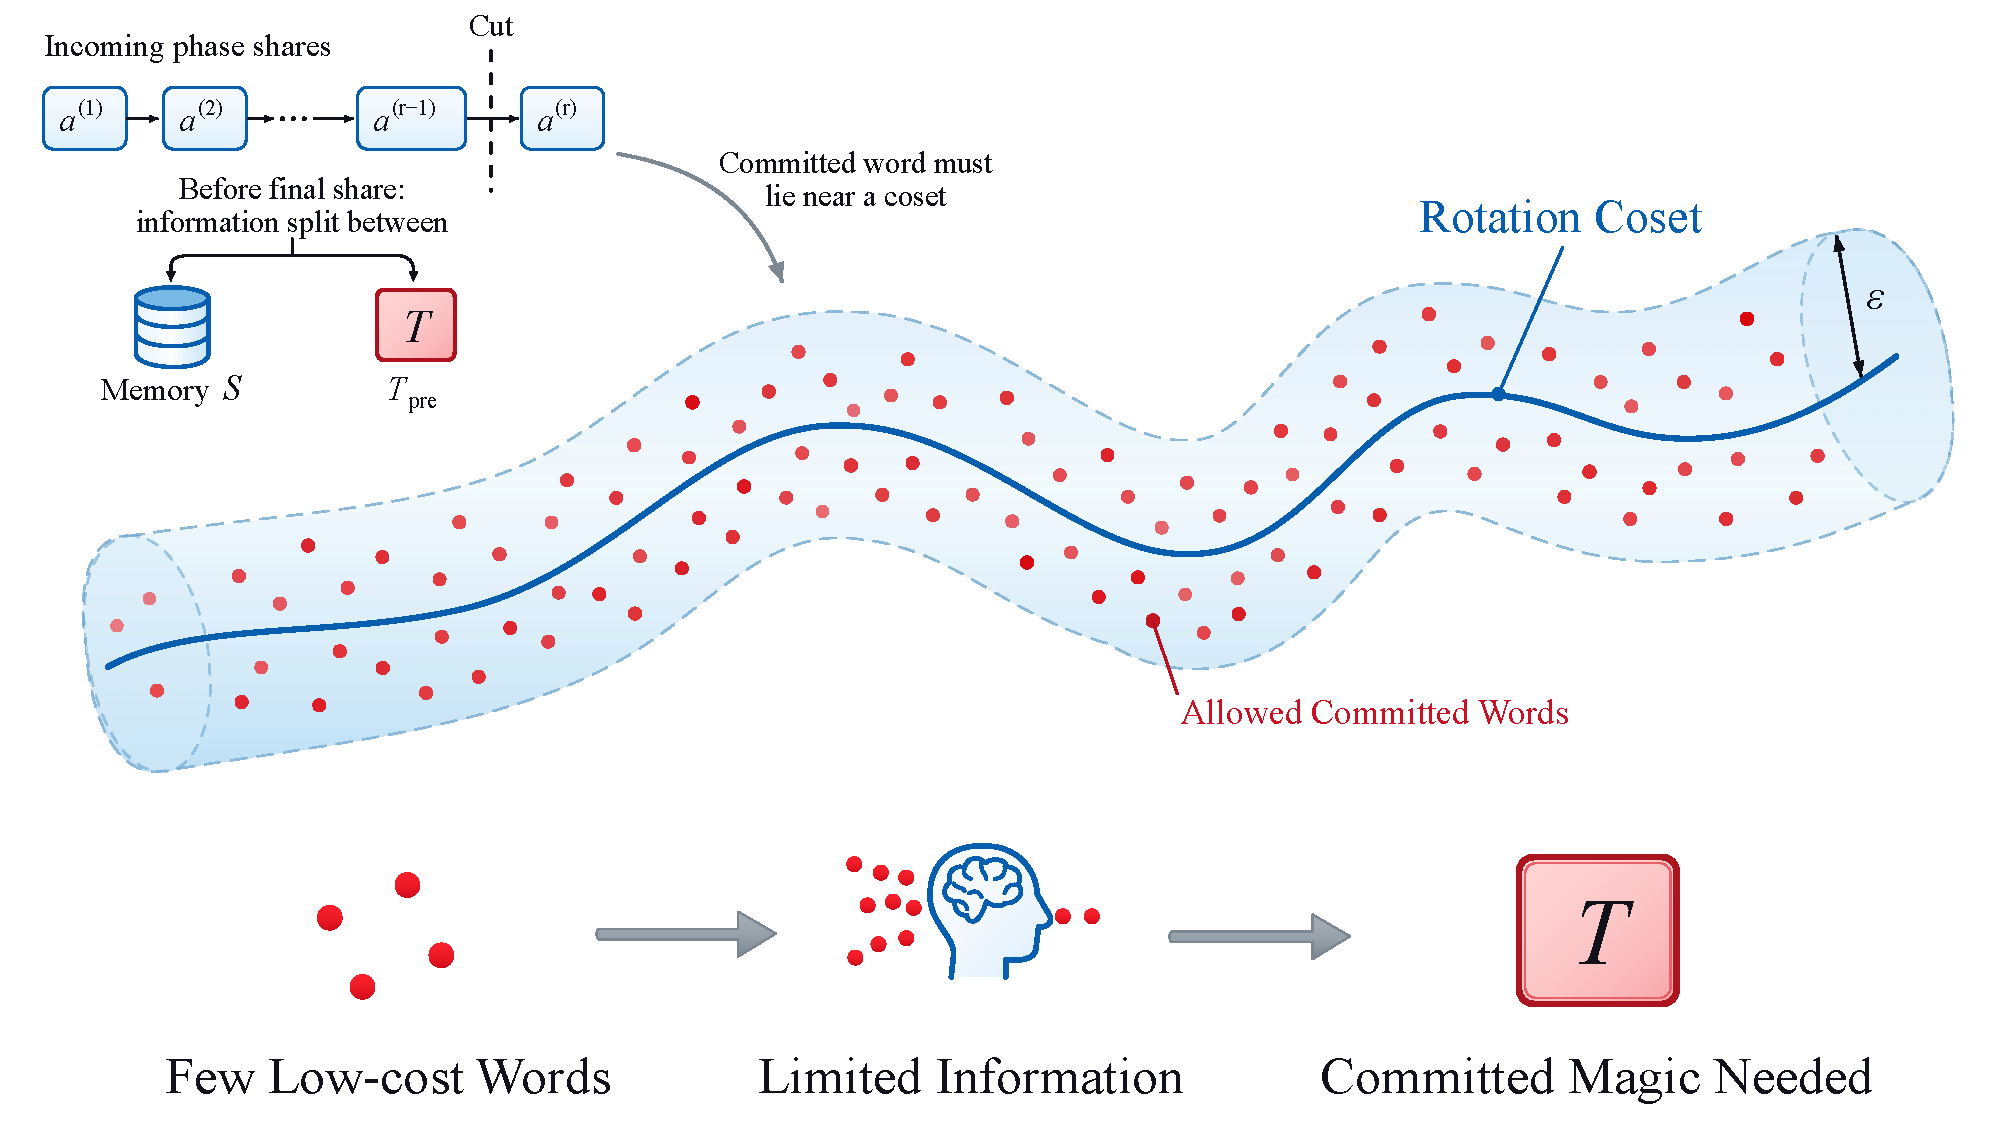
\includegraphics[width=0.92\textwidth]{fig0_schematic.pdf}
\caption{Why committed magic is charged per bit (schematic, not to scale). Top left: the shares $a^{(1)},\dots,a^{(r)}$ of a phase arrive in rounds, and at the last inter-round cut, before the final share, the information about the aggregate is split between the snapshot $S$ carried in memory and the $T$ gates $\Tpre$ already committed. Centre: a committed word must lie within $\varepsilon$ of a rotation coset $G_1R_z(\theta)G_2$, a curve (blue) of codimension $\beta=2$ in $\SU$, and the tube of radius $\varepsilon$ around it contains few Clifford+$T$ words of low $T$-count (red), at most $C_12^k\varepsilon^2+C_2(k+1)2^{k/2}$ of $T$-count $\le k$ (Theorem~\ref{thm:tube}). Bottom: few low-cost words means that a cheap committed word carries little information about its coordinate, so every bit not held in memory must be paid for in committed magic.}
\label{fig:schematic}
\end{figure*}


\paragraph{What is new.} Relative to~\cite{Paper1}, whose bit-level bound Theorem~\ref{thm:main1} reproves with the Matsumoto--Amano count in place of Kraft's inequality, the new unconditional results are the count of Clifford+$T$ words near a rotation coset with explicit constants (Theorem~\ref{thm:tube}), the rates $2$, $\tfrac52$ and $3$ (Theorems~\ref{thm:rate2}, \ref{thm:rate52} and~\ref{thm:rate3seg}) and the volume law at Clifford cosets (Theorem~\ref{thm:clifford}). The counting results of~\cite{PS18} bound covering exponents in the whole group, and Selinger's~\cite[Thm.~30]{Selinger15} bounds the worst-case cost of one angle; neither controls how many cheap words lie near a coset, which is what a streaming lower bound needs. We are not aware of an earlier bound below the square-root barrier of the spectral method for points of this $S$-arithmetic quaternion lattice near an arbitrary rotation coset; for points of spheres near planes and in caps see~\cite{BourgainRudnick}, and for optimal strong approximation~\cite{BKS,Sardari}. Theorem~\ref{thm:frontier} is an elementary construction whose rate depends on a synthesis hypothesis, and Theorem~\ref{thm:main2} is conditional on Conjecture~\ref{conj:H}, whose exponent is fixed by geometry and whose constants we test but do not prove.

Sec.~\ref{sec:setting} states the model, Sec.~\ref{sec:results} the results, Sec.~\ref{sec:num} the numerical evidence and Sec.~\ref{sec:models} the dependence on the model; Sec.~\ref{sec:disc} discusses them. All proofs are in the appendices. Extended numerics, and the results of Sec.~\ref{sec:models} with their proofs, are in the Supplemental Material~\cite{SM}.


\section{Setting}\label{sec:setting}

The model is the streaming compilation model of~\cite{Paper1}. So that the present paper can be read on its own, Appendix~\ref{app:model} restates the four items we use---the charged one-pass process and its snapshots, the dispersed family, the closed form of the projective distance, and the block compiler---as Definitions~\ref{def:model} and~\ref{def:family}, Lemma~\ref{lem:dproj} and Proposition~\ref{prop:block}, with proofs. Nothing below depends on any other result of~\cite{Paper1}; in particular Theorem~\ref{thm:main1} reproves its bit-level bound.

\paragraph{Family.} Fix a modulus $Q\ge3$, step $\Delta=2\pi/Q$, alphabet size $K=Q-1$, and $m$ $\F_2$-independent $Z$-characters $P_1,\dots,P_m$ on $n\ge m$ qubits; let $V$ be a fixed public Clifford with $VZ_jV^\dagger=P_j$. The aggregate is $x\in[K]^m$, $[K]=\{0,\dots,K-1\}$, and the target is
\begin{equation}
U_x=V\Big(\bigotimes_{j\le m}R_z(\Delta x_j)\otimes I\Big)V^\dagger,\qquad R_z(\theta)=e^{-i\theta Z/2}.
\end{equation}
An $r$-round dispersed stream is a round-major sequence of shares $a^{(1)},\dots,a^{(r)}\in\Z_Q^m$ with $\sum_ta^{(t)}\equiv x\pmod Q$. The \emph{canonical sharing} $\mathcal D$ takes $a^{(1)},\dots,a^{(r-1)}$ i.i.d.\ uniform on $\Z_Q^m$ and $a^{(r)}=x-\sum_{t<r}a^{(t)}$. The accuracy satisfies $0<\varepsilon<\sin(\pi/2Q)$, so that distinct grid rotations are separated by $2\sin(\pi/2Q)>2\varepsilon$ in the projective distance $\dproj(A,B)=\inf_\phi\|A-e^{i\phi}B\|$ and nearest-grid decoding is unambiguous. The \emph{tuned} modulus $Q_\varepsilon:=\lfloor\pi/(2\arcsin2\varepsilon)\rfloor$ is the largest for which the separation is at least $4\varepsilon$; it satisfies $\log_2K_\varepsilon=L-\log_2(4/\pi)+o(1)=L-0.35+o(1)$, where throughout
\begin{equation}
L:=\log_2(1/\varepsilon).
\end{equation}

\paragraph{Output model.} The \emph{coordinatewise ancilla-free Clifford+$T$ model} (CW) is the one realized by per-rotation synthesis pipelines, in which each generator of the phase polynomial is handed to a single-qubit synthesizer and no ancilla or cross-coordinate cancellation is used~\cite{RossSelinger,Paper1}: the write-once output is a list of records $(j,g)$ with $j\in[m]$ and $g\in\{H,S,T\}$, the implemented unitary is $V(\bigotimes_jW_j)V^\dagger$ where $W_j$ is the ordered product of the gates recorded on coordinate $j$, and the $T$-count is the number of $T$ records. We say the output is \emph{correct} if $\dproj(W_j,R_z(\Delta x_j))\le\varepsilon$ for every $j$. By Lemma~\ref{lem:loc}, correctness of the whole unitary---$\dproj(V(\bigotimes_jW_j)V^\dagger,U_x)\le\varepsilon$, the criterion of~\cite{Paper1}---implies coordinatewise correctness, so every lower bound below also holds under the total criterion. The converse is not asserted: a construction with coordinate error $\varepsilon$ need only have total error at most $m\varepsilon$, and for a total error budget $\varepsilon_{\mathrm{tot}}$ the share-by-share construction of Sec.~\ref{sec:frontier} can use $\varepsilon_{\mathrm{tot}}/(mr)$ per share.

\paragraph{Process and committed magic.} The process is a compiler in the charged one-pass model of Definition~\ref{def:model}: it reads the stream once, may use arbitrary RAM and a random tape whose state is part of every restart snapshot, and $S:=\max_{\text{input}}\E_\rho\max_cB_{\mathrm{cut}}(c)$ is the worst-input expected snapshot size. It is required to be correct with probability $\ge1-\delta$ on every $x$ and every valid stream, $\delta<\tfrac12$. Let $T_t$ be the number of $T$ records emitted while reading round $t$, $\Tpre:=\sum_{t<r}T_t$ the \emph{committed magic}, and $\Tout=\Tpre+T_r$. Bars denote expectation over the tape, the canonical sharing and a uniform aggregate. We write $L_\delta(m,K):=(1-\delta)m\log_2K-h_2(\delta)$, $\ell_\delta:=(1-\delta)\log_2K-h_2(\delta)$, and $\rho_m(\bar T):=m\log_2(e(1+\bar T/m))+2\log_2(1+\bar T)+1$.

\paragraph{A concrete instance.} A program contains $m$ mutually commuting and independent Pauli rotations $e^{-\mathrm i\theta_jP_j/2}$, as in Pauli-based computation~\cite{Litinski}, and each angle receives contributions $\theta_j=\sum_t\theta^{(t)}_j$ from $r$ segments separated by operations that commute with every $P_j$, so that contributions to the same $P_j$ may be merged. The angles are computed at run time by the classical host from mid-circuit measurement outcomes, as in adaptive and feedback circuits, and segment $t$ must be lowered into the append-only instruction stream before segment $t+1$ exists~\cite{Caune,Fowler}. Rounding to the grid of $Q_\varepsilon$ gives the shares, $V$ is a Clifford with $VZ_jV^\dagger=P_j$, and a back end that hands every rotation it emits to a single-qubit synthesizer~\cite{RossSelinger} is a CW process; it is rotation-segmented in the sense of Sec.~\ref{sec:seg}. Its only freedom is the merging policy: a contribution can be held as a running sum modulo $Q$, at $\lceil\log_2Q\rceil$ bits of snapshot per Pauli, or emitted on arrival. For $r=2$, $\varepsilon=10^{-10}$ and $m=10^4$, holding everything costs $S\approx41$\,kB and no committed magic; emitting everything commits $105.34$ $T$ gates per Pauli on average, each share synthesized to $\varepsilon/2$; and no zero-error CW back end with $S=0$, whatever it emits, commits fewer than $25.72$ per Pauli on average (Table~\ref{tab:numbers}). These averages are over the canonical sharing, i.e.\ over run-time angles whose earlier contributions are uniform on the grid and independent of the total; for any other joint law, $m\log_2K$ is replaced by the entropy that the back end is missing at the cut (Theorem~\ref{S:thm:side}).


\section{Results}\label{sec:results}

All proofs are in the appendices. Appendix~\ref{app:lemmas} collects the elementary lemmas used throughout; among them Lemma~\ref{lem:MA}, the Matsumoto--Amano count of $36\cdot2^t$ words of $T$-count $t$, is the source of the rate one.

\subsection{Committed magic}\label{sec:main1}

\begin{theorem}[Committed magic]\label{thm:main1}
For every process as in Sec.~\ref{sec:setting} and every round $t\in[r-1]$,
\begin{equation}\label{eq:main1}
S+\bar T_t+m\log_236+\rho_m(\bar T_t)\ \ge\ L_\delta(m,K).
\end{equation}
Consequently
\begin{multline}
\bar\Tpre\ \ge\ (r-1)\big[L_\delta(m,K)-S-m\log_236\big]\\-(r-1)\,\rho_m\!\Big(\frac{\bar\Tpre}{r-1}\Big),
\end{multline}
and for the tuned family and $\delta=0$, $\Tpre\ge(r-1)(m\log_2K_\varepsilon-S)-O(rm\log\log(1/\varepsilon))$.
\end{theorem}
Theorem~\ref{thm:main1} is the bit-level theorem of~\cite{Paper1} with Lemma~\ref{lem:MA} in place of Kraft's inequality: one committed $T$ gate per bit not held, per round (Appendix~\ref{app:main1}). Its lower bounds, and all those below, do not depend on the target.

\begin{corollary}[Commitment before cancellation is knowable]\label{cor:identity}
Under the canonical sharing $\mathcal D$ the rounds $a^{(1)},\dots,a^{(r-1)}$ are i.i.d.\ uniform and independent of the aggregate $x$, and $\Tpre$ is a function of $(a^{(1)},\dots,a^{(r-1)},\rho)$ alone. Hence for every fixed aggregate $x\in[K]^m$,
\[
\E\big[\Tpre\,\big|\,X=x\big]=\bar\Tpre ,
\]
and the lower bounds of Theorems~\ref{thm:main1}, \ref{thm:rate2}, \ref{thm:rate52}, \ref{thm:rate3seg} and~\ref{thm:main2}, and those of Theorems~\ref{thm:rate115} and~\ref{thm:rate177} in Appendix~\ref{app:beyond}, hold after conditioning on $X=0$, for which $U_x=I$. A process that is required to be correct on every valid stream, and is not promised in advance that the aggregate vanishes, commits the same expected magic whether or not the phases cancel.
\end{corollary}
The corollary is a restatement of the sharing distribution, not an independent strengthening: a compiler told the promise $X=0$ can emit nothing, and the statement concerns the resources a universally correct process has already spent on a stream that turns out to cancel.

\subsection{Words near rotation cosets: the rate two}\label{sec:tube}

Single-qubit Clifford+$T$ modulo phase is an $S$-arithmetic group $\Gamma$ acting on the $3$-regular Bruhat--Tits tree, with $T$-count equal to tree distance~\cite{KMM13,PS18}. We write $\Lambda_k\subset\Gamma$ for the ball of $T$-count $\le k$ and (R) for the Ramanujan bound $\|T_j\|\le(j+1)2^{j/2}$ on the Hecke operators of this lattice~\cite{LPS,PS18}, which is a theorem (Appendix~\ref{app:tube}).


\begin{theorem}[Tube bound]\label{thm:tube}
For all $G_1,G_2\in\SU$, all $\varepsilon\in(0,1/8]$ and all $k\ge0$, with
$T_\varepsilon(C):=\{W:\exists\theta,\ \dproj(W,G_1R_z(\theta)G_2)\le\varepsilon\}$,
\begin{equation}\label{eq:tube}
\#\big(\Lambda_k\cap T_\varepsilon(C)\big)\ \le\ C_1\,2^k\varepsilon^2+C_2\,(k+1)\,2^{k/2},
\end{equation}
with the absolute constants $C_1=72\cdot4\sqrt2\le408$ and $C_2=24(1-2^{-1/2})^{-1}2^{3/2}\le232$.
\end{theorem}
The proof (Appendix~\ref{app:tube}) reduces the tube to a spherical cap via the Hopf fibration whose fibre is the coset, majorizes the cap by a Poisson kernel of width $2\varepsilon$---whose spherical-harmonic coefficients are $r^\ell$ with $1-r=2\varepsilon$, so that both constants can be read off---and bounds the count by the Hecke operator through a rank-one sup-norm estimate.
The error term $(k+1)2^{k/2}$ cannot be reduced by this method, and it exceeds the main term in the whole range $k\le4L$ in which synthesized rotations live (Remark~\ref{rem:barrier}); proving that the true count is the main term is the content of Conjecture~\ref{conj:H} below.


\begin{theorem}[Rate two]\label{thm:rate2}
Under (R), put $n(\tau):=C_12^\tau\varepsilon^2+C_2(\tau+1)2^{\tau/2}$, $\tau_*:=\lceil2\log_2K\rceil$ and
\begin{equation}\label{eq:A2}
A_2:=1+\log_2 Z,\qquad Z:=\sum_{\tau\le\tau_*}n(\tau)2^{-\tau/2},
\end{equation}
so that $A_2=\log_2C_2+2\log_2(2\log_2K)+O(1)=O(\log\log(1/\varepsilon))$. Then for every round $t$,
\begin{equation}
\bar T_t\ \ge\ 2\big[(1-2\delta)m\log_2K-2m\,h_2(\delta)-S-mA_2\big],
\end{equation}
hence $\bar\Tpre\ge2(r-1)[(1-2\delta)m\log_2K-2mh_2(\delta)-S-mA_2]$.
\end{theorem}
Given the snapshot and the other rounds, a committed word of $T$-count $\tau$ carries at most $\tau/2+A_2$ bits about its coordinate (Appendix~\ref{app:rate}). The additive term is not negligible in practice: at $\varepsilon=10^{-10}$, $A_2=20.0$ of the $32.9$ bits a coordinate carries.

\subsection{Beyond the square-root barrier: the rate five halves}\label{sec:rate52}

The square-root remainder of Theorem~\ref{thm:tube} is a limit of the spectral method, not of the problem. A determinant method in the style of Bombieri--Pila and Heath-Brown~\cite{BombieriPila,HeathBrown}, adapted as in the cap lemmas of Bourgain--Rudnick~\cite{BourgainRudnick}, uses no automorphic input and no arithmetic property of the frame. It lifts each word to its quaternion numerator, a lattice point on a sphere of radius $\asymp2^{t/4}$ in both real embeddings of $\Q(\sqrt2)$, cuts the tube into boxes, and shows that the affine determinant of any five points of a box vanishes, so that the points of a box lie on a round $2$-sphere. One determinant per box gives the rate $\tfrac{11}5$; splitting the sphere sections by the height of their hyperplane gives $\tfrac{17}7$; fibring the numerators over rational planes and projections, with the resulting case analysis checked exactly by an SMT solver on a continuum of box shapes, gives every rate below $\tfrac52$ (Appendices~\ref{app:beyond}--\ref{app:rate52}).


\begin{theorem}[Rate five halves]\label{thm:rate52}
For every $\alpha<\tfrac52$ there is $L_0(\alpha)$ such that, for every process as in Sec.~\ref{sec:setting}, every round $t<r$ and every $L\ge L_0(\alpha)$,
\begin{multline}\label{eq:rate52}
\bar T_t\ \ge\ \alpha\big[(1-2\delta)m\log_2K-2m\,h_2(\delta)\\-S-mA\big],\qquad A=O_\alpha(1).
\end{multline}
Behind it is the following tube bound. For every $0<\mu\le\tfrac1{10}$ there is $\eta_\mu(t)=o(t)$ such that, for all $G_1,G_2\in\SU$, all $\varepsilon\in(0,1/8]$ and all $t\le4(L+2)/(\tfrac85+\mu)$, with $C=G_1R_zG_2$,
\begin{equation}\label{eq:rate52tube}
\#\{W:\ t_{\min}(W)\le t,\ W\in T_\varepsilon(C)\}\ \le\ 2^{(\frac25-\frac\mu{11})t+\eta_\mu(t)}.
\end{equation}
\end{theorem}
Near the limit the exponent $\tfrac25-\tfrac\mu{11}$ is sharp for this case analysis, so the method approaches $\tfrac52$ but does not reach it. This is where it stops: $\tfrac52$ is where its boxes shrink to $\varepsilon$-cubes, and a tube carrying words of $T$-count $(\tfrac52+o(1))L$ with gaps of at most $2^{o(L)}$ grid steps along its core would make $\tfrac52$ sharp (Proposition~\ref{prop:dense}). Theorem~\ref{thm:rate52} does not use (R) and holds uniformly over frames. It is a statement about the rate: its additive term and its $L_0(\alpha)$ are not explicit, and Theorem~\ref{thm:rate2} remains the bound we evaluate in Sec.~\ref{sec:num}.

\subsection{An achievable tradeoff family}\label{sec:frontier}


\begin{theorem}[Fractional passthrough]\label{thm:frontier}
For every $q\in\{0,\dots,m\}$ and every single-rotation synthesizer of cost $\tau(\varepsilon)$ per rotation to projective error $\varepsilon$, there is a deterministic zero-error one-pass CW process with
\begin{align}
S&\le\lceil q\log_2Q\rceil+O(\log(mQr)),\notag\\
T_t&\le(m-q)\,\tau(\varepsilon/r)\quad(t<r),\notag\\
\Tout&\le\big(m+(r-1)(m-q)\big)\,\tau(\varepsilon/r).
\end{align}
\end{theorem}
Under the canonical sharing every pre-final share is uniform on $\Z_Q$, so the expected committed magic of this process is exactly $(r-1)(m-q)\,\bar\tau_Q(\varepsilon/r)$, with $\bar\tau_Q$ the mean synthesis cost on the grid (Corollary~\ref{cor:frontier}). If $\bar\tau_Q(\varepsilon/r)=(3+o(1))\log_2K$---which Ross--Selinger synthesis gives for a typical angle, $\tau=3L+O(\log L)$~\cite{RossSelinger}, and which Sec.~\ref{sec:num} measures on the grid at $\varepsilon=10^{-10}$---the family has asymptotic slope $3$. It is not optimal for the first bits of a coordinate: when $8\mid Q$, two are shed for free and a third for half a $T$ gate on average (Remark~\ref{rem:firstbit}).

\subsection{Rotation-segmented processes: the rate three}\label{sec:seg}

At the cosets whose frame is Clifford the volume law holds up to a subexponential factor: there the off-diagonal entry of a word is an arithmetic coordinate, and the divisor bound controls the rest.


\begin{theorem}[Volume law at Clifford cosets]\label{thm:clifford}
There is $\eta(\tau)=O(\tau/\log\tau)$ such that for all Cliffords $C_1,C_2$, all $\varepsilon\in(0,1/8]$ and all $\tau\ge1$, with $C=C_1R_zC_2$,
\begin{equation}\label{eq:clifford}
\#\{W:\ t_{\min}(W)\le\tau,\ W\in T_\varepsilon(C)\}\le2^{\eta(\tau)}\big(\tau+1+\varepsilon^22^\tau\big).
\end{equation}
For $G_1,G_2\in\Gamma$ with $t_{\min}(G_1)+t_{\min}(G_2)\le h$ the same holds with $\tau$ replaced by $\tau+h$.
\end{theorem}
\begin{corollary}[Typical $z$-rotations need $3L$]\label{cor:typical}
For every $\varepsilon\in(0,1/8]$ and every $s\ge0$, the set of $\theta\in[0,4\pi)$ for which $R_z(\theta)$ has an $\varepsilon$-approximation of $T$-count $\le3L-s$ has measure $\le C\,2^{\eta(3L)}\big(L2^{-L}+2^{-s}\big)$. The same bound holds for the fraction of grid angles $2\pi d/Q$, $d\in\Z_Q$, for the tuned modulus $Q=Q_\varepsilon$ and for any modulus $Q\ge c'/\varepsilon$ with $\sin(\pi/2Q)>\varepsilon$.
\end{corollary}
In words, all but a vanishing fraction of $z$-rotations need $T$-count $3L-O(L/\log L)$, which is the lower half of~\cite[Conj.~8.10]{RossSelinger} for almost every angle; the passthrough family cannot be improved by a better single-rotation synthesizer, only by a better way of committing.


Theorem~\ref{thm:clifford} also bounds the processes that pipelines actually run. Call a CW process \emph{$\vartheta$-rotation-segmented} if, on every input and tape, for every coordinate $j$ and every round $t<r$, the unitary $\overline W^{(t)}_j$ of the segment it emits on $j$ in round $t$ is within $\vartheta$ of $C\,R_z(\varphi)\,C'$ for some angle $\varphi$ and some Cliffords $C,C'$. Per-rotation synthesis of each share is of this form, and so is the fractional-passthrough family of Theorem~\ref{thm:frontier}, with $\vartheta=\varepsilon/r$. The constraint bears on the committed word itself, so the frames of Corollary~\ref{cor:profile}, which are the source of the gap between Theorems~\ref{thm:rate52} and~\ref{thm:main2}, play no role.

\begin{theorem}[Rate three for rotation-segmented processes]\label{thm:rate3seg}
For every $\vartheta$-rotation-segmented process as in Sec.~\ref{sec:setting} with $\vartheta\le1/8$, and every round $t<r$,
\begin{multline}\label{eq:rate3seg}
\bar T_t\ \ge\ \alpha_\vartheta\big[(1-2\delta)m\log_2K-2m\,h_2(\delta)\\-S-mA_\vartheta\big],\qquad\alpha_\vartheta:=1+\frac{2\log_2(1/\vartheta)}{\log_2K},
\end{multline}
with $A_\vartheta=O(\Lambda/\log\Lambda)$, $\Lambda:=\alpha_\vartheta\log_2K$. In particular, a $\vartheta$-rotation-segmented process with $\vartheta\le\varepsilon$ is $\varepsilon$-rotation-segmented, and $\alpha_\varepsilon\ge3-O(1/L)$, so $\bar\Tpre\ge3(r-1)\big(m\log_2K-S-O(mL/\log L)\big)-O(\delta rmL)$.
\end{theorem}
Theorem~\ref{thm:rate3seg} matches the passthrough family in its rate: in the model where each committed piece is within $\varepsilon$ of a Clifford-framed $z$-rotation, the exchange rate is $3$ to leading order in $L$, unconditionally from below and from above under the synthesis hypothesis of Sec.~\ref{sec:frontier}. Like Theorem~\ref{thm:rate52} it is asymptotic; its additive term is controlled by the worst-case divisor bound and is vacuous at $\varepsilon=10^{-10}$ (Appendix~\ref{app:clifford}). Beating it requires committing words that are not near any Clifford-framed rotation and whose frames, created by the prefix and suffix, carry the rest of the information. Theorem~\ref{thm:rate52} bounds how much such frames can help, and Conjecture~\ref{conj:H} asserts that they cannot help at all.

\subsection{Rate three under an equidistribution conjecture}\label{sec:conj}


\begin{conjecture}[H]\label{conj:H}
There are constants $c_0,c_1,c$ such that for all $G_1,G_2\in\SU$, all $\varepsilon\in(0,1/8]$, all moduli $3\le Q\le Q_\varepsilon$ (i.e.\ $\sin(\pi/2Q)\ge2\varepsilon$, the separation of the tuned family) and all $\tau\ge0$,
\begin{multline}\label{eq:H}
\#\big\{W:\ t_{\min}(W)\le\tau,\ \exists d\in\Z_Q:\\ \dproj\big(W,G_1R_z(\tfrac{2\pi d}{Q})G_2\big)\le\varepsilon\big\}\\ \le\ c_0+c_1\tau+c\,2^\tau\varepsilon^{\beta},\qquad\beta=2 .
\end{multline}
\end{conjecture}
The exponent $\beta$ is the codimension of a rotation coset in the three-dimensional group, and the linear term is forced: a coset can lie within $\varepsilon$ of every power of an infinite-order word (Proposition~\ref{prop:cluster}). We do not fix the constants. A finite scan bounds $c$ from below and never from above, and the largest requirement we know is $c\ge163.9$ if $(c_0,c_1)=(8,2)$ (Sec.~\ref{sec:num}); where a number is needed we assume $(c_0,c_1,c)=(8,2,256)$, an additional assumption that is above every requirement we know. By Theorem~\ref{thm:clifford} the conjecture holds at Clifford cosets up to $2^{O(\tau/\log\tau)}$, and it implies that no ancilla-free synthesis of grid rotations beats the Ross--Selinger exponent (Appendix~\ref{app:conj}).


\begin{theorem}[Rate three; quantization]\label{thm:main2}
Assume Conjecture~\ref{conj:H}, $Q\le Q_\varepsilon$ and $\varepsilon\le(2c)^{-1/2}$. Put $k:=\log_2K$, $b:=\beta L-\log_2c-1$, $\tau_0:=\lfloor\beta L-\log_2c\rfloor$, $N_0:=c_0+c_1\tau_0+1$, $a_0:=1+\log_2N_0$, $\kappa:=1+b/k$ and $D_t:=(1-2\delta)mk-2mh_2(\delta)-S$. For every round $t<r$,
\begin{equation}\label{eq:rate3}
\bar T_t\ \ge\ \kappa\,(D_t-ma_0)-3m\log_2(1+\bar T_t/m),
\end{equation}
and, writing $\bar{\mathcal A}^{>}_t$ for the expected number of coordinates that are correct and whose word committed in round $t$ has minimal $T$-count greater than $\tau_0$,
\begin{equation}\label{eq:active}
\bar{\mathcal A}^{>}_t\ \ge\ \frac{D_t-ma_0}{k}.
\end{equation}
\end{theorem}
For every fixed $c$, $\kappa\to1+\beta=3$, so $\bar\Tpre\ge3(r-1)(m\log_2K-S)(1-o(1))-O(rm\log L)$. The structural content is quantization: a committed word of cost at most $\tau_0=\lfloor2L-\log_2c\rfloor$ carries at most $\log_2N_0=O(\log L)$ bits about its coordinate, and~\eqref{eq:active} counts how many coordinates per round must commit a word of cost $\ge2L-O(1)$, so memory should be shed in whole rotations rather than in low bits. The convergence is slow: at $\varepsilon=10^{-10}$ and $c=256$, $\tau_0=58$, the allowance is $7.0$ of the $32.9$ bits a coordinate carries, and $\kappa=2.75$ (Appendix~\ref{app:conj}).


\section{Numerical evidence}\label{sec:num}

We enumerated all single-qubit Clifford+$T$ unitaries of $T$-count $\le22$ ($3.0\times10^8$ words) through the Matsumoto--Amano normal form. Details, two further tables and the scripts are in Sec.~\ref{S:sec:numsupp} of the Supplemental Material~\cite{SM}.

\paragraph{Equidistribution near rotation cosets (Fig.~\ref{fig:tube}).} For $\varepsilon\in\{2^{-4},\dots,2^{-8}\}$ with tuned moduli $Q_\varepsilon\in\{12,25,50,100,201\}$, on the identity coset and on two Haar-random cosets, a least-squares fit over the $136$ cells with count $\ge30$ gives $\log_2N=1.001\,t-2.007\,L+\text{const}$, the exponents $(1,\beta)=(1,2)$ of Conjecture~\ref{conj:H} to three decimals. The constants are not fitted: on the $30$ Haar-pair cells whose expected count exceeds $3000$, the counts divided by the exact Haar prediction lie in $[0.98,1.04]$ for the grid and in $[0.98,1.01]$ for the tube. Four arithmetic frames, built from Clifford+$T$ words of $T$-count $0$, $5$, $10$ and $15$, give the same exponents. Clifford cosets are isometric copies of the identity coset, which is below Haar at low cost---the fee---and overshoots for a few $T$-counts above the onset $t\approx2L$. These overshoots set the size of $c$: the axis coset of $HT$ requires $c\ge53.5$, and the identity coset at the non-dyadic accuracy $\varepsilon=0.024532$ requires $c\ge163.9$ if $(c_0,c_1)=(8,2)$, which is why Table~\ref{tab:numbers} and Fig.~\ref{fig:frontier} use $c=256$.


\begin{figure*}[t]
\centering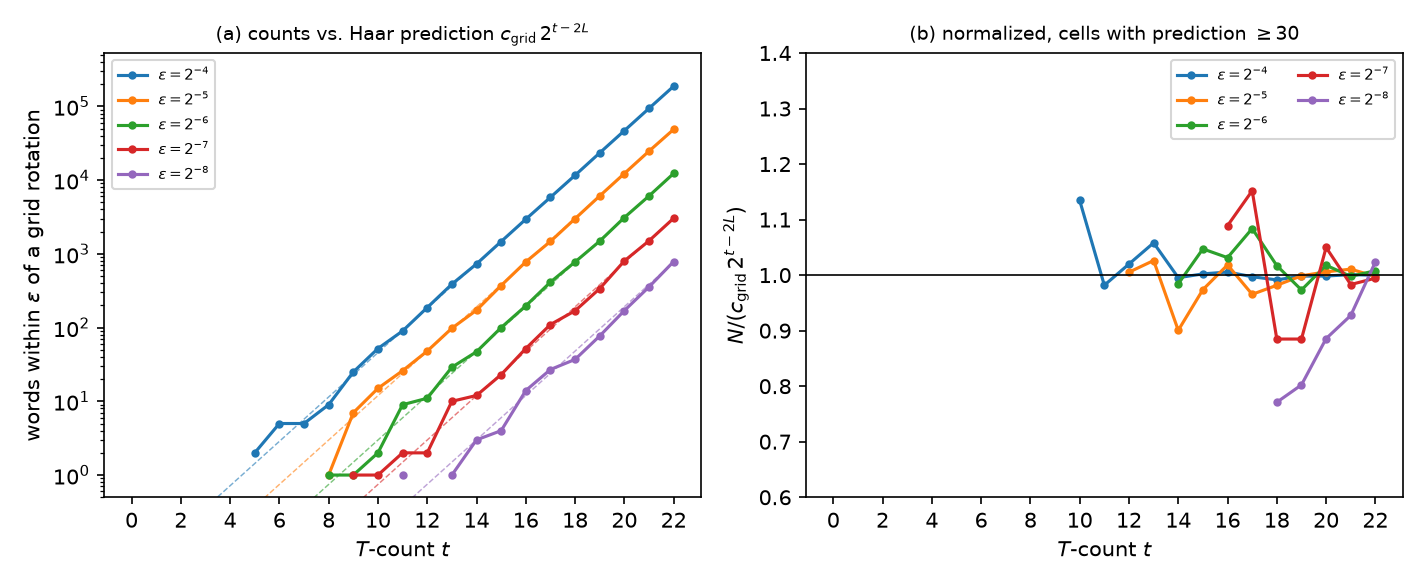
\includegraphics[width=0.92\textwidth]{fig1_tube_counts.png}
\caption{Number of Clifford+$T$ words of $T$-count exactly $t$ within $\varepsilon$ of a grid rotation on a Haar-random coset $G_1R_z(\theta)G_2$. (a) Counts (markers) against the exact Haar prediction $c_{\mathrm{grid}}2^{t-2L}$ with $c_{\mathrm{grid}}=48\varepsilon Q_\varepsilon/\pi$ (dashed). (b) The same counts divided by that prediction, plotted where the prediction is at least $30$; every $\varepsilon$ has reached the Haar value by $t=22$. Exhaustive enumeration to $t=22$ ($3.0\times10^8$ words, $1.5\times10^8$ in the top shell).}
\label{fig:tube}
\end{figure*}

\paragraph{Synthesis cost and the bounds (Fig.~\ref{fig:frontier}, Table~\ref{tab:numbers}).} For $L\le6$ the enumeration gives the exact minimal $T$-count of every grid rotation; at the share accuracy $\varepsilon/2$ that Theorem~\ref{thm:frontier} certifies for $r=2$, the passthrough slopes are $3.333$ and $3.334$ at $L=5$ and $6$. At $\varepsilon=10^{-10}$ we synthesize $20\,000$ uniform grid angles with Ross--Selinger synthesis: $\E\tau=102.32$ at $\varepsilon$ ($3.113$ per bit) and $105.34$ at $\varepsilon/2$ ($3.205$ per bit). Committing only the low $\ell$ bits of a share costs between $4.5$ and $20$ times the passthrough slope per bit shed, because in this model a rotation by any nonzero grid angle costs a full synthesis: the quantum of commitment persists at scale. Table~\ref{tab:numbers} evaluates the bounds with all constants. At $S=0$ the rigorous floors are $21.75\,m$ (Theorem~\ref{thm:main1}) and $25.72\,m$ (Theorem~\ref{thm:rate2}) committed $T$ gates per round, the conditional one is $51.3\,m$, and passthrough achieves $105.34\,m$; the rate-two bound exceeds the rate-one bound only for $S<3.7\,m$ bits.


\begin{table}[t]
\centering\footnotesize
\caption{The bounds at $\varepsilon=10^{-10}$ ($L=33.22$, $Q_\varepsilon=7\,853\,981\,633$, $\log_2K=32.871$), per coordinate per round, at $S=0$. ``Coeff.'' is the leading coefficient of $-S$ in the bound (for the bounds of Theorems~\ref{thm:main1} and~\ref{thm:main2} the finite-precision derivative $-\partial\bar T_t/\partial S$ at $S=0$ is $0.94$ and $2.54$, because of their logarithmic terms); ``per bit'' is $\bar T_t/(m\log_2K)$ at $S=0$. The achievable row is the fractional-passthrough family with each committed share synthesized at $\varepsilon/2$, the accuracy Theorem~\ref{thm:frontier} requires for $r=2$; the single-rotation calibration at $\varepsilon$ is $102.32$. The Theorem~\ref{thm:main2} row assumes that Conjecture~\ref{conj:H} holds with $(c_0,c_1,c)=(8,2,256)$; $c=256$ is above the largest requirement we know ($c\ge163.9$, Sec.~\ref{sec:num}) but is not proven to suffice, and at $c=163.9$ the row would read $51.7$.}
\label{tab:numbers}
\setlength{\tabcolsep}{4pt}\begin{tabular}{@{}l ccc@{}}
\toprule
& $\bar T_t/m$ & per bit & coeff.\\
\midrule
Thm.~\ref{thm:main1} (unconditional) & $21.75$ & $0.66$ & $1$\\
Thm.~\ref{thm:rate2} (given (R)) & $25.72$ & $0.78$ & $2$\\
Thm.~\ref{thm:main2} (Conj.~\ref{conj:H}, $c=256$) & $51.3$ & $1.56$ & $\kappa=2.75$\\
achievable (Thm.~\ref{thm:frontier}) & $105.34$ & $3.20$ & $3.205$\\
\quad(\texttt{gridsynth} at $\varepsilon/2$) & & &\\
\bottomrule
\end{tabular}
\end{table}

\begin{figure*}[t]
\centering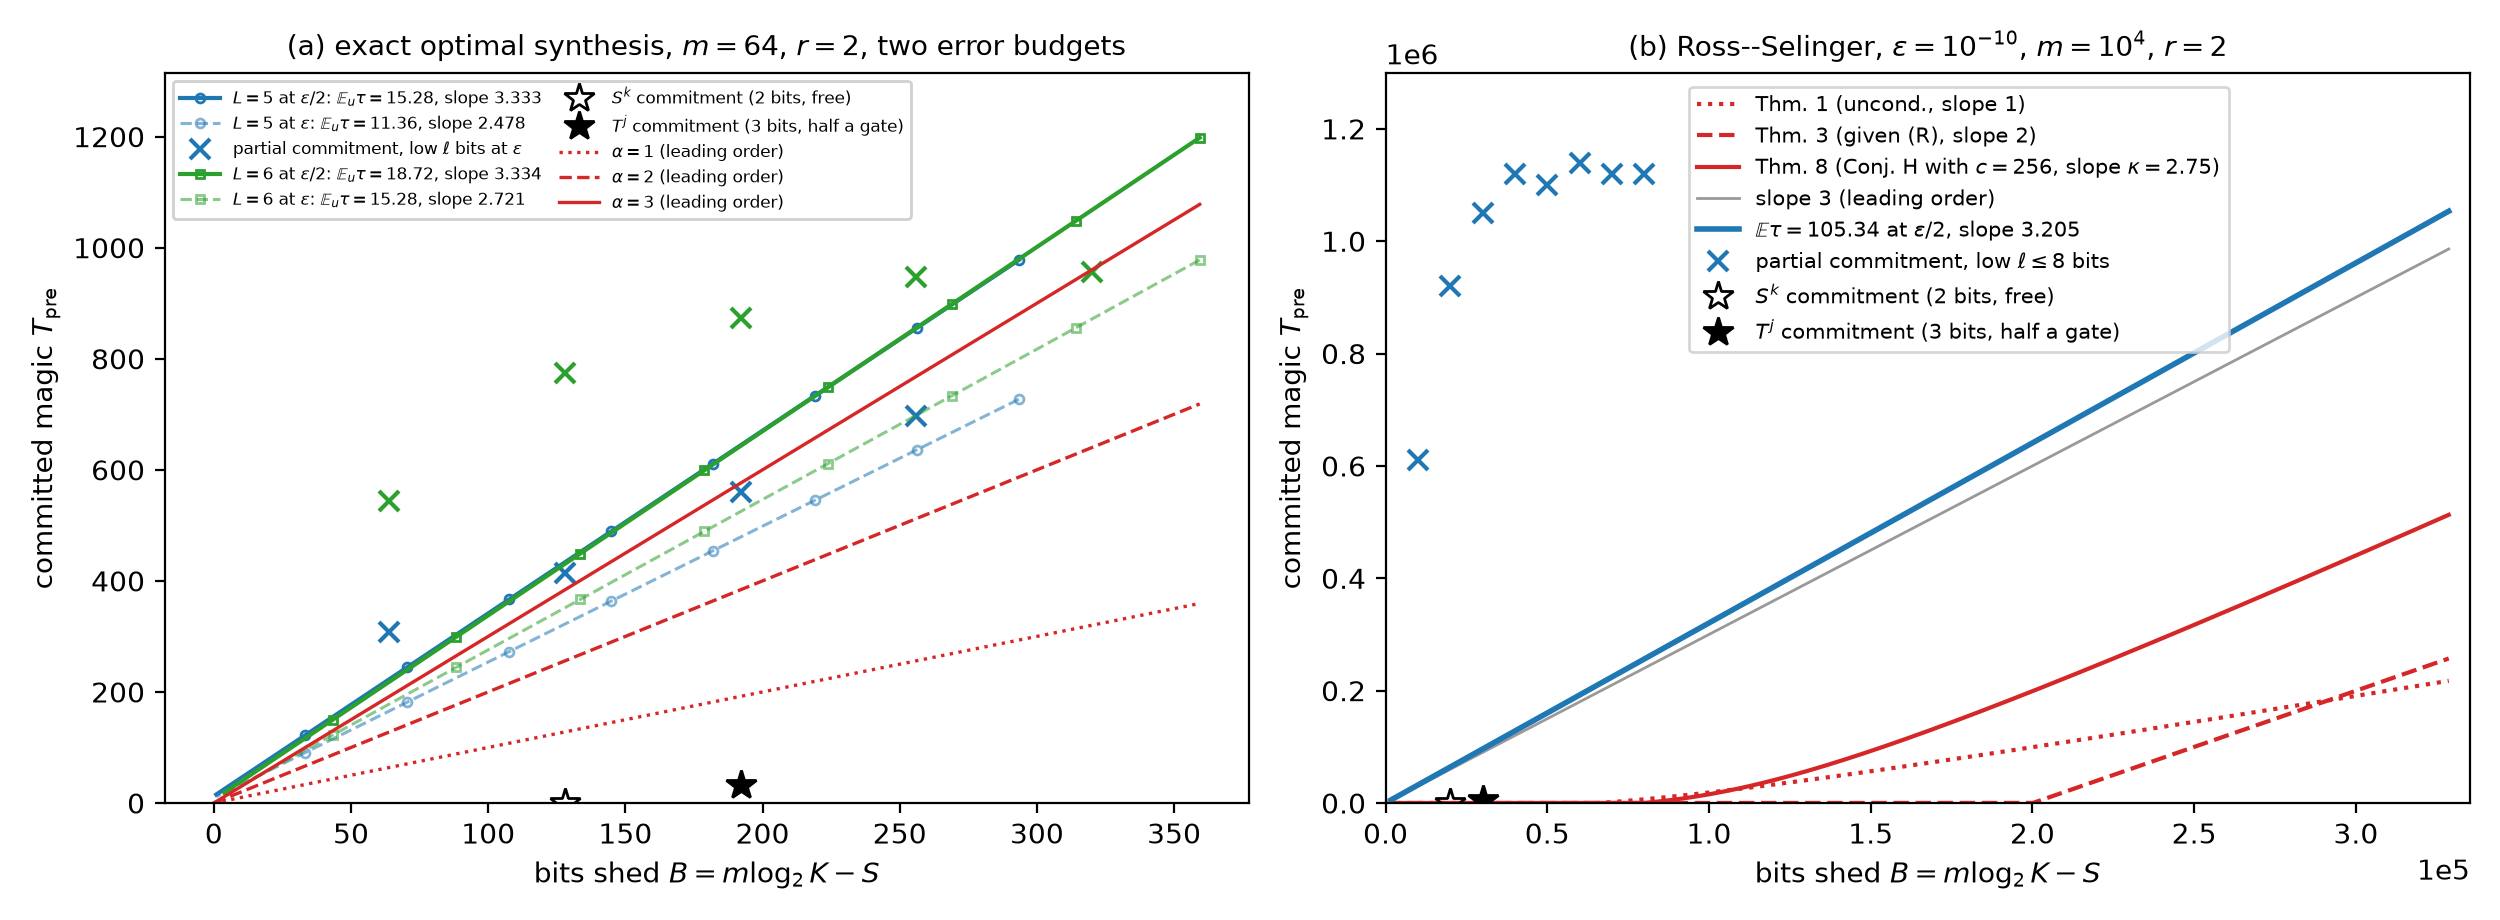
\includegraphics[width=0.92\textwidth]{fig2_frontier_twopanel.png}
\caption{The fractional-passthrough tradeoff family ($r=2$) against the lower bounds. (a) Exact minimal $T$-counts from the enumeration, $m=64$, $L=5,6$---an optimum no synthesis algorithm can beat---against the leading-order slopes $\alpha=1,2,3$; at $L\le6$ the additive terms swamp the main terms, all three bounds being vacuous, so only slopes can be compared there. Solid: the committed piece synthesized at $\varepsilon/2$, the accuracy Theorem~\ref{thm:frontier} requires for $r=2$, which is the family the theorem bounds. Dashed: the same optima at word accuracy $\varepsilon$, a single-rotation calibration and not a point of the family. The two budgets straddle $\alpha=3$---slopes $3.333$ and $3.334$ above it, $2.478$ and $2.721$ below---and the $\varepsilon/2$ slopes at $L=5$ and $6$ coincide to three decimals. (b) Ross--Selinger synthesis at $\varepsilon=10^{-10}$, $m=10^4$, from $20\,000$ sampled grid rotations, against those three bounds as stated, intercepts included (Table~\ref{tab:numbers}; the rate-three line is Theorem~\ref{thm:main2} assuming Conjecture~\ref{conj:H} with $(c_0,c_1,c)=(8,2,256)$, intercept $51.3\,m$; $c=256$ is above the largest requirement we know, $c\ge163.9$, but is not proven to suffice); the achievable line is the $\varepsilon/2$ point $\E\tau=105.34$; the grey line is the leading-order slope $3$, for comparison. The rate-two bound (dashed) overtakes the rate-one bound (dotted) only near the right-hand end, $S<3.7\,m$ bits. Crosses: partial commitment of the low $\ell$ bits of each share, committed piece synthesized at $\varepsilon$ in both panels. Star: the exact commitment of Remark~\ref{rem:firstbit} on the grid $Q=8\lfloor Q_\varepsilon/8\rfloor$, three bits per coordinate for half a $T$ gate (the first two of them free). Its abscissa is $2-\log_2\frac{Q}{Q-1}$ and $3-\log_2\frac{Q}{Q-1}$ rather than exactly $2$ and $3$ ($2.9386$ for the third bit at $Q=24$); points taken on different moduli are all plotted as $\log_2(Q-1)-S/m$.}
\label{fig:frontier}
\end{figure*}

\section{Beyond the coordinatewise model}\label{sec:models}

The lower bounds above concern the CW model, and Secs.~\ref{S:sec:side}--\ref{S:sec:mixing} of the Supplemental Material~\cite{SM} determine how they change in neighbouring models; Table~\ref{S:tab:models} there compares the rates. We summarize.

\paragraph{Side information.} If the process holds side information $Y$ from the start, or the shares have any joint law with the aggregate, $m\log_2K$ in Theorem~\ref{thm:main1} is replaced by the conditional entropy $H(X\mid\mathrm{Past},\mathrm{Fut},Y)$ (Theorem~\ref{S:thm:side}). A process that holds the seed of a randomized-compiling twirl faces no obstruction, and one that misses an injective $\lambda$-bit seed independent of the aggregate is charged for at most $\lambda$ bits rather than $m\log_2K$: this is the precise boundary of the ``randomize and lower late'' rule of~\cite{Paper1} (Corollary~\ref{S:cor:side}).

\paragraph{Probabilistic mixing.} If committed words are sampled at run time from programs, as in mixed-channel synthesis~\cite{Campbell17,Hastings17,KLMPP,Bothe}, a committed word need only be accurate to $\sqrt\varepsilon$. The law is rescaled and not removed: all but the top $\tfrac12L+O(\log L)$ bits of every share are free, the remaining bits are charged in total at the same rate, and a coordinate that is not held still costs at least $L-O(\log L)$ committed $T$ gates per round, against $\tfrac32L$ achievable under a synthesis hypothesis (Theorem~\ref{S:thm:mixing}, Corollary~\ref{S:cor:mixstop}, Proposition~\ref{S:prop:mixach}); under Conjecture~\ref{conj:H} the rate is again $3$ per coarse bit, with fee $L-O(1)$ (Corollary~\ref{S:cor:mixq}). Quasi-probabilistic mixtures, whose resource is sample overhead, are not covered.

\paragraph{Measurement adaptivity.} Repeat-until-success and fallback synthesis with $n-1$ ancillas keep a floor of order $L/n$ on the number of $T$ gates plus measurements per share not held (Proposition~\ref{S:prop:adaptive}).

\paragraph{Ancillas and batching.} Ancillas that survive a cut are memory and must be charged as such, so the meaningful model has clean ancillas. With clean ancillas and a catalytic phase-gradient register prepared once, table lookups batched over $g\asymp\log L$ coordinates commit a share for $O(L/\log L)$ $T$ gates when $\log L=o(m)$ (Proposition~\ref{S:prop:batch}), so no constant-rate law survives batching across coordinates; at $\varepsilon=10^{-10}$ batching saves about $40\%$, not an order of magnitude. The constant-rate law is a statement about coordinatewise synthesis, which is what per-rotation pipelines implement.

\section{Discussion}\label{sec:disc}

In the model where rotations are synthesized coordinate by coordinate without ancillas, a bit of aggregate phase information that a schedule does not carry across a round boundary costs at least two committed magic states with explicit constants and at least $\tfrac52-o(1)$ asymptotically, at least $3-o(1)$ when every committed piece is $\varepsilon$-close to a Clifford-framed rotation, and three suffice along the passthrough family whenever the grid-mean synthesis cost is $(3+o(1))L$---asymptotically in $L$, and after the first $O(\log L)$ bits of each coordinate. Three is a volume count: a rotation coset has codimension $\beta=2$ in $\SU$, so a word pays $\beta L$ gates to enter the tube around it and one gate per bit thereafter. Two is what the spectral method yields: the Ramanujan bound controls the tube only up to an error $2^{\tau/2}$, the square root of the number of all words of that cost. Five halves is the exact limit of the determinant method with one auxiliary hyperplane per box, because $\tfrac52$ is where a box of the five-point determinant has shrunk to an $\varepsilon$-cube; going beyond it means showing that most $\varepsilon$-cubes along a tube are empty, and by Proposition~\ref{prop:dense} it requires at least excluding tubes that carry words of $T$-count $(\tfrac52+o(1))L$ with gaps of at most $2^{o(L)}$ grid steps along their core. Heuristically, arguments that cover a tube by balls cannot pass $\tfrac52$ (Sec.~\ref{S:sec:what52} of~\cite{SM}), and, as far as we can see, the standard square-root inputs---the Ramanujan bound, or a twisted Linnik conjecture of the kind that gives optimal strong approximation on $S^3$~\cite{BKS}---stop at rate $2$ in their natural circle-method and spectral implementations. Whether the true rate for general processes is $3$ is not decided here; Conjecture~\ref{conj:H}, which the enumeration supports on Haar-random, arithmetic and Clifford cosets, is the statement that the arithmetic words do not know the difference.

Three consequences are worth stating plainly. First, the corner $S=0$ is where the law binds without anyone choosing to be memoryless. When the rotation angles are produced on the quantum side---qubitization, a QROM-loaded phase table, adaptive QSVT phases---no classical snapshot of them exists to be traded away; our proof applies Fano's inequality to a classical stream and does not reach that case, which is the natural target for this line of work. Second, memory cannot be traded for magic in small units inside a coordinate, and which units are available is a property of the synthesis mechanism, not of magic. With deterministic words the trade is quantized in whole rotations under Conjecture~\ref{conj:H} (Theorem~\ref{thm:main2}), and Ross--Selinger synthesis at $\varepsilon=10^{-10}$ puts the penalty for shedding low bits at $4.5$ to $20$ times the passthrough slope; with probabilistic mixing the low $\tfrac12L-\tfrac12\log_2L-O(1)$ bits of every share are free~\cite{Bothe}, and above them, under Conjecture~\ref{conj:H}, whole coordinates should again be shed (Corollary~\ref{S:cor:mixq}). Third, side information enters at the level of a conditional entropy: randomization raises the cost of commitment only for a compiler that does not hold the seed.

Two unconditional statements bound the arithmetic question from the other side: Selinger's worst-case $T$-count $4L-9$ for a specific $z$-rotation~\cite[Thm.~30]{Selinger15}, and the covering exponents of Parzanchevski and Sarnak, who show that some single-qubit unitaries need $T$-count $4L$ while all are reachable at $6L$~\cite{PS18}. The committed-magic frontier is a statement about the typical rather than the worst case, and it sits between the rigorous and the conjectural covering exponents in the same way. Closing the gap between $\tfrac52$ and $1+\beta$ for committed words with arbitrary frames is the remaining problem.


\begin{acknowledgments}
J.Y.'s deepest thanks go to two teachers who are also coauthors of this
paper, Yangyang Li and Xiu-Hao Deng. Their help was immense; without them
this paper would not exist.

J.Y. thanks Ke Lin of Xidian University for opening the door to research
and for the recommendation that led him to join Prof.~Li's group.

J.Y. also thanks the teachers who were willing to offer guidance along the
way, and the senior members of Prof.~Li's group, who have been generous
with their help throughout this work.

Thanks are due, finally, to everyone who supported this paper, too many to
name individually here.

Y.L. acknowledges support from the National Natural Science Foundation of
China under Grant No.~62476209, the Key Research and Development Program of
Shaanxi under Grant No.~2024CY2-GJHX-18, and the Fundamental Research Funds
for the Central Universities under Grant No.~QTZX26097. X.-H.D.
acknowledges support from the Science, Technology and Innovation Commission of Shenzhen
Municipality (Grant Nos.~JCYJ20170412152620376 and KYTDPT20181011104202253),
the Innovation Program for Quantum Science and Technology (Grant
No.~2021ZD0301703), the Guangdong Major Project of Basic Research (Grant
No.~2025B0303000007), and the Shenzhen Science and Technology Program
(Grant No.~KQTD20200820113010023).

Generative AI tools were used to assist with manuscript drafting and
revision, code and repository maintenance, literature discovery, and
consistency checks. The authors directed their use through task-specific
prompts and independently reviewed the generated text, citations, code, and
numerical claims against the cited literature, source files, executable tests,
and the exact rational certificates reported in this work. AI output was
not treated as a scientific source or as independent proof verification. The
authors take full responsibility for the manuscript, proofs, code, data,
figures, citations, and conclusions.
\end{acknowledgments}

\section*{Author contributions}
J.Y. developed the theory and proofs, implemented the enumeration, synthesis and certificate code, and performed
the numerical computations and analyses. Y.L. supervised the research, reviewed and revised the manuscript,
and provided project administration and funding support. H.L. contributed to
data visualization and helped compile the literature and organize the numerical data. X.-H.D.
independently validated the theoretical derivations, numerical results, and
computational artifacts. All authors wrote the manuscript together,
discussed the results, and approved the final version.

\section*{Data availability}
{\raggedright
The exhaustive enumeration of Clifford+$T$ words to $T$-count $22$, the coset counts of Table~\ref{S:tab:counts} and Fig.~\ref{fig:tube}, the exact-optimal and \texttt{gridsynth} data of Fig.~\ref{fig:frontier}, and every script that produces a number or figure of this paper are available at \url{https://github.com/OIerYangJZ/memory-magic-exchange-law}. The scripts are in \texttt{scripts/}, among them \texttt{enum2.py} and \texttt{enum\_arith.py} (the enumeration and coset counts), \texttt{gridsynth\_run.py}, \texttt{fig1\_fig.py} and \texttt{make\_fig2.py} (the figures), \texttt{thm\_numbers.py} (Table~\ref{tab:numbers}), \texttt{mixing\_bounds.py} (the constants of Sec.~\ref{S:sec:mixing} of the Supplemental Material) and \texttt{scan2.py}, \texttt{scan2\_report.py} and \texttt{astra1.py} (the frame scans of Sec.~\ref{S:sec:numsupp} of the Supplemental Material). The exact rational certificates of Appendices~\ref{app:elem} and~\ref{app:dioph} are \texttt{research/cert/certificate.py}, \texttt{research/cert/certificate\_223.py} and \texttt{research/dioph/cert\_dioph.py}. The exact certificate of Appendix~\ref{app:proj} is \texttt{research/annulus/cert\_proj.py}, and the continuum model and SMT check of Appendix~\ref{app:rate52} are \texttt{research/uniform52/cont\_model.py} and \texttt{research/uniform52/verify\_z3.py}, with the solver output in \texttt{research/uniform52/z3\_outputs.txt}. The example of Remark~\ref{S:rem:what52} of the Supplemental Material is reproduced by \texttt{research/conditional3/ballpts.cpp} (\texttt{ballpts 25 5.828427 1 1 -1 0.0025}) and \texttt{research/conditional3/review/check\_sections.py}. The repository README lists, for every table, figure and theorem, the script and data file that produce it.\par}


\appendix

\section{The streaming model}\label{app:model}

This appendix states the four items of~\cite{Paper1} that the main text and the Supplemental Material use, in the form in which they are used, with proofs, so that the present paper can be refereed on its own. The definitions are those of~\cite[Def.~9, 13, 20, 21]{Paper1} and the two statements are~\cite[Lem.~1, Prop.~10]{Paper1}; no other result of~\cite{Paper1} is used anywhere above.

\begin{definition}[Charged one-pass process]\label{def:model}
A \emph{charged one-pass process} on the stream $a^{(1)},\dots,a^{(r)}$ is an algorithm with a random tape $\rho$ and a write-once output tape such that
\begin{enumerate}\setlength\itemsep{0pt}
\item[(i)] it reads the stream once, in order, and may keep unbounded internal state while reading a round;
\item[(ii)] at each \emph{cut} $c$ between consecutive rounds it emits a \emph{snapshot} $\sigma_c$, a finite bit string, with the \emph{restart} property: everything the process writes after $c$ is a function of $\sigma_c$ and of the part of the stream after $c$. The tape $\rho$ is part of $\sigma_c$, so a process that wishes to reuse its randomness pays for it;
\item[(iii)] snapshots are serialized in a prefix-free code, whence $H(\sigma_c)\le\E|\sigma_c|$;
\item[(iv)] its \emph{charge} is $S:=\max_{\mathrm{input}}\E_\rho\max_cB_{\mathrm{cut}}(c)$, where $B_{\mathrm{cut}}(c):=|\sigma_c|$.
\end{enumerate}
For $p>1$ passes the process may re-read the stream $p$ times, and the object playing the role of $\sigma_c$ is the transcript of all $2p-1$ crossings of the cut.
\end{definition}
Condition (iii) is free: prefixing a snapshot with its own length in Elias-$\gamma$ makes any serialization prefix-free at a cost of $2\log_2(|\sigma_c|+1)+1$ bits, which is dominated by the $O(\log(mQr))$ terms of every construction below. Condition (ii) is the only substantive one, and it is what an append-only instruction stream enforces: the process may not revise what it has already emitted, and what it has not written down it must remember.

\begin{definition}[Dispersed family, canonical sharing, tuned modulus]\label{def:family}
With $Q,\Delta,K,m,V,P_j,U_x$ as in Sec.~\ref{sec:setting}, an \emph{$r$-round dispersed stream} for the aggregate $x\in[K]^m$ is any $a^{(1)},\dots,a^{(r)}\in\Z_Q^m$ with $\sum_ta^{(t)}\equiv x\pmod Q$; correctness is required on every such stream, not only on typical ones. The \emph{canonical sharing} $\mathcal D$ draws $a^{(1)},\dots,a^{(r-1)}$ i.i.d.\ uniform on $\Z_Q^m$ and sets $a^{(r)}:=x-\sum_{t<r}a^{(t)}$. The \emph{tuned} modulus at accuracy $\varepsilon$ is $Q_\varepsilon:=\lfloor\pi/(2\arcsin2\varepsilon)\rfloor$.
\end{definition}

\begin{lemma}[Tuned modulus]\label{lem:tuned}
For $0<\varepsilon\le1/8$ one has $Q_\varepsilon\ge6$, $\sin(\pi/2Q_\varepsilon)\ge2\varepsilon$, and $\log_2K_\varepsilon=L-\log_2(4/\pi)+o(1)=L-0.35+o(1)$.
\end{lemma}
\begin{proof}
$Q_\varepsilon\le\pi/(2\arcsin2\varepsilon)$ gives $\pi/2Q_\varepsilon\ge\arcsin2\varepsilon$, i.e.\ $\sin(\pi/2Q_\varepsilon)\ge2\varepsilon$, which is the accuracy condition of Sec.~\ref{sec:setting} with a factor $2$ to spare; $\varepsilon\le1/8$ gives $\arcsin2\varepsilon\le\arcsin\tfrac14<\pi/12$ and so $Q_\varepsilon\ge6$. Since $\arcsin2\varepsilon=2\varepsilon(1+O(\varepsilon^2))$, $Q_\varepsilon=\pi/(4\varepsilon)+O(1)$ and $\log_2K_\varepsilon=\log_2(Q_\varepsilon-1)=L+\log_2(\pi/4)+o(1)$.
\end{proof}

\begin{lemma}[Projective distance]\label{lem:dproj}
For unitaries $A,B$ of equal size, $\dproj(A,B)=2\sin(\Theta/4)$, where $\Theta\in[0,2\pi]$ is the length of the shortest closed arc of the unit circle containing $\spec(B^\dagger A)$.
\end{lemma}
\begin{proof}
By unitary invariance of the operator norm,
\[\dproj(A,B)=\inf_\phi\|B^\dagger A-e^{i\phi}I\|=\inf_\phi\max_{\lambda\in\spec(B^\dagger A)}|\lambda-e^{i\phi}|,\]
since $B^\dagger A$ is normal. Write $d(\phi,\lambda)\in[0,\pi]$ for angular distance, so that $|\lambda-e^{i\phi}|=2\sin(d(\phi,\lambda)/2)$, increasing in $d$. If $e^{i\phi_0}$ is the midpoint of a shortest arc, every eigenvalue is within $\Theta/2$ of it and the two ends attain that, so the maximum equals $2\sin(\Theta/4)$. Conversely, for any $\phi$ put $D:=\max_\lambda d(\phi,\lambda)\le\pi$; the spectrum then lies in the closed arc of length $2D$ centred at $e^{i\phi}$, so $\Theta\le2D$ by minimality and $\max_\lambda|\lambda-e^{i\phi}|=2\sin(D/2)\ge2\sin(\Theta/4)$.
\end{proof}

\begin{proposition}[Block compiler]\label{prop:block}
For every $q\le m$ there is a deterministic one-pass process which, on every $r$-round dispersed stream, keeps the running sums modulo $Q$ of $q$ designated coordinates in a snapshot of at most $\lceil q\log_2Q\rceil+O(\log(mQr))$ bits and, at round $r$, knows the exact aggregate $x_j$ of each designated coordinate.
\end{proposition}
\begin{proof}
The state carried across a cut is the vector of partial sums in $\Z_Q^q$, encoded as one integer in $[Q^q]$, i.e.\ $\lceil q\log_2Q\rceil$ bits; the remainder of the snapshot is the round index, the position within the round and a fixed-size program counter, $O(\log(mQr))$ bits, made prefix-free as in Definition~\ref{def:model}\,(iii). The designated set is fixed in advance and need not be stored. Each arriving share is added modulo $Q$ into its partial sum, so after round $r$ the $j$-th sum is $\sum_ta^{(t)}_j\bmod Q=x_j$.
\end{proof}
The gap between $\log_2Q$ here and the $\log_2K$ of the lower bounds is the difference between storing a share, which ranges over $\Z_Q$, and the entropy of an aggregate, which ranges over $[K]$; it is $\log_2(Q/K)=O(1/Q)$ per stored coordinate.

\section{Lemmas}\label{app:lemmas}


\begin{lemma}[Localization]\label{lem:loc}
For unitaries $A=\bigotimes_jA_j$, $B=\bigotimes_jB_j$ on the same tensor factors,
\[\max_j\dproj(A_j,B_j)\le\dproj(A,B)\le\sum_j\dproj(A_j,B_j).\]
For $2\times2$ unitaries, $\dproj(A,B)=\sqrt{2-|\tr(B^\dagger A)|}$.
\end{lemma}

\begin{lemma}[Matsumoto--Amano count]\label{lem:MA}
The number of single-qubit Clifford+$T$ unitaries modulo phase of minimal $T$-count exactly $t$ is $n_1(0)=24$ and $n_1(t)=36\cdot2^t$ for $t\ge1$; hence $\sum_{s\le t}n_1(s)=72\cdot2^t-48$, and the number of $m$-tuples with total minimal $T$-count at most $T$ is $N^{\le}_m(T)\le36^m2^T\binom{T+m}{m}$.
\end{lemma}

\begin{lemma}[Entropy versus $T$-count]\label{lem:ent}
Let $M=(\overline W_1,\allowbreak\dots,\allowbreak\overline W_m)$ be a random $m$-tuple of single-qubit Clifford+$T$ unitaries and $T\ge\sum_jt_{\min}(\overline W_j)$ a random integer. Then $H(M)\le\bar T+m\log_236+\rho_m(\bar T)$.
\end{lemma}

\begin{lemma}[Identity coset]\label{lem:identity}
If $2\varepsilon^24^k<1$, i.e.\ $k<L-\tfrac12$, the only Clifford+$T$ unitaries with denominator exponent $\le k$ within $\varepsilon$ of some $R_z(\theta)$ are the eight powers of $T$.
\end{lemma}
Lemma~\ref{lem:MA} is the source of the exchange rate: a $T$ gate carries at most $\log_22=1$ bit. Lemma~\ref{lem:identity} is an elementary instance of the entry fee (Appendix~\ref{app:conj}).


\begin{proof}[Proof of Lemma~\ref{lem:loc}]
By Lemma~\ref{lem:dproj}, $\dproj(A,B)=2\sin(\Theta/4)$ where $\Theta\in[0,2\pi]$ is the length of the shortest closed arc containing $\spec(B^\dagger A)$. The spectrum of $\bigotimes_jB_j^\dagger A_j$ consists of the products of eigenvalues. Fix $j$ and two eigenvalues $\lambda,\lambda'$ of $B_j^\dagger A_j$ at circular distance $\theta_j\le\pi$; multiplying both by a fixed product $\mu$ of eigenvalues of the other factors gives two points of the joint spectrum at circular distance $\theta_j$, and any closed arc containing both has length at least $\theta_j$. Hence $\Theta\ge\theta_j$, and since $\sin$ increases on $[0,\pi/2]$, $\dproj(A,B)\ge2\sin(\theta_j/4)=\dproj(A_j,B_j)$. For the right inequality replace one factor at a time: $\|\bigotimes A_j-e^{i\sum\phi_j}\bigotimes B_j\|\le\sum_j\|A_j-e^{i\phi_j}B_j\|$, then take infima. For the closed form, with eigenphases $a,b$ of $B^\dagger A$ one has $|\tr|^2=2+2\cos\Theta$ and $2\sin(\Theta/4)=\sqrt{2-2\cos(\Theta/2)}=\sqrt{2-|\tr|}$, using $\cos(\Theta/2)\ge0$ for $\Theta\le\pi$.
\end{proof}

\begin{proof}[Proof of Lemma~\ref{lem:MA}]
Every Clifford+$T$ unitary has a unique normal form $(T|\epsilon)(HT|SHT)^*C$ with $C$ one of the $24$ Cliffords modulo phase~\cite{MA08}, and the normal form is $T$-optimal~\cite{KMM13}. Strings with exactly $t$ letters $T$ number $2^{t-1}$ (initial $T$ present) plus $2^t$ (absent), times $24$. For tuples, $\prod_jn_1(t_j)\le36^m2^{\sum_jt_j}$ and the number of $(t_j)$ with $\sum t_j\le T$ is $\binom{T+m}{m}$.
\end{proof}

\begin{proof}[Proof of Lemma~\ref{lem:ent}]
Encode $M$ by the Elias-$\gamma$ code of $T$ (at most $2\log_2(T+1)+1$ bits) followed by an index among $N^{\le}_m(T)$ tuples; $H(M)$ is at most the expected length of this prefix code. Use $\log_2\binom{T+m}{m}\le m\log_2(e(1+T/m))$, which is concave in $T$, and Jensen.
\end{proof}

\begin{proof}[Proof of Lemma~\ref{lem:identity}]
Write the unitary as
\[2^{-k/2}\begin{pmatrix}u&-t^\dagger\omega^l\\ t&u^\dagger\omega^l\end{pmatrix}\]
with $u,t\in\Z[\omega]$, $\omega=e^{i\pi/4}$, $uu^\dagger+tt^\dagger=2^k$~\cite{KMM13}. By the closed form of Lemma~\ref{lem:loc}, closeness to a diagonal unitary forces $|t|^2\le2\varepsilon^22^k$. The Galois conjugate $\sqrt2\mapsto-\sqrt2$ of the norm equation gives $|t^\bullet|^2\le2^k$. Hence $\xi:=tt^\dagger\in\Z[\sqrt2]$ is totally non-negative with $N_{\Q(\sqrt2)/\Q}(\xi)=\xi\xi^\bullet\le2\varepsilon^24^k<1$, which forces $\xi=0$ and $t=0$. Then $uu^\dagger=2^k$; the prime above $2$ in $\Z[\omega]$ is $(1-\omega)$ with $(1-\omega)^4\sim2$, and the units of relative norm one are the $\omega^j$, so $u=\omega^j(1-\omega)^{2k}$ times a unit and the unitary is $\operatorname{diag}(\omega^a,\omega^b)$ modulo phase.
\end{proof}

\section{Proof of Theorem~\ref{thm:main1} and Corollary~\ref{cor:identity}}\label{app:main1}

\begin{proof}[Proof of Theorem~\ref{thm:main1}]
Fix $t$. Let $A:=a^{(t)}$, $\mathrm{Past}:=(a^{(s)})_{s<t}$, $\mathrm{Fut}:=(a^{(s)})_{s>t}$ (which includes round $r$), and $Z:=(\mathrm{Past},\mathrm{Fut},\rho)$.

\emph{(i) $H(A\mid Z)=m\log_2K$.} Under $\mathcal D$ the joint law of $(a^{(1..r-1)},x)$ is $Q^{-m(r-1)}P_X(x)$ with $a^{(r)}$ determined. Conditioning on $(\mathrm{Past},\mathrm{Fut})$ fixes $c:=\sum_{s\ne t}a^{(s)}$ and $x=A+c$, so the conditional law of $A$ is proportional to $P_X(A+c)$, i.e.\ uniform on the translate $[K]^m-c$. The tape is independent of the stream.

\emph{(ii) Message and Fano.} Let $M_t:=(\overline W^{(t)}_1,\dots,\overline W^{(t)}_m)$ be the tuple of unitaries (modulo phase) implemented by the gate segments emitted on the respective coordinates during round $t$, and $\sigma_t$ the restart snapshot at the cut after round $t$. Given $\rho$ the process is deterministic; the segments emitted before round $t$ are a function of $(\mathrm{Past},\rho)$, and those emitted after the cut are a function of $(\sigma_t,\mathrm{Fut})$ by the restart semantics of Definition~\ref{def:model}\,(ii). Hence the final unitary on coordinate $j$, $U^{<t}_j\overline W^{(t)}_jU^{>t}_j$, is a function of $(M_t,\sigma_t,Z)$. On success it is within $\varepsilon$ of $R_z(\Delta x_j)$, and nearest-grid decoding recovers $x_j$ because neighbouring grid rotations are more than $2\varepsilon$ apart; thus $A=x-c$ is recovered with error probability $\le\delta$. Fano's inequality gives $H(A\mid M_t,\sigma_t,Z)\le h_2(\delta)+\delta\log_2(K^m-1)$, i.e.\ $I(A;M_t,\sigma_t\mid Z)\ge L_\delta(m,K)$.

\emph{(iii) Message size.} $I(A;M_t,\sigma_t\mid Z)\le H(\sigma_t)+H(M_t)$. The snapshot serialization is prefix-free (Definition~\ref{def:model}\,(iii)), so $H(\sigma_t)\le\E|\sigma_t|\le S$, the worst-input expectation dominating the average over inputs. The number $T_t$ of $T$ records emitted in round $t$ is at least $\sum_jt_{\min}(\overline W^{(t)}_j)$, so Lemma~\ref{lem:ent} gives $H(M_t)\le\bar T_t+m\log_236+\rho_m(\bar T_t)$. This proves~\eqref{eq:main1}; summing over $t$ and using concavity of $\rho_m$ proves the rest.
\end{proof}

\begin{remark}[Multiple passes]
For $p$ forward passes, the alternating-simulation transcript---all $2p-1$ crossing snapshots together with the unitary tuple committed while scanning rounds $<r$ in any pass, cut between rounds $<r$ and round $r$ as in~\cite{Paper1}---determines the output, and the same argument gives $\Sigma_p+\bar T_A+m\log_236+\rho_m(\bar T_A)\ge L_\delta$ with $\Sigma_p\le(2p-1)S$. The per-round splitting, and with it the factor $r-1$, is a one-pass phenomenon: a process that rereads round $t$ after seeing round $r$ need not commit anything during round $t$.
\end{remark}

\begin{proof}[Proof of Corollary~\ref{cor:identity}]
Independence is item (i) of the proof of Theorem~\ref{thm:main1}; $\Tpre$ counts records emitted while reading rounds $<r$, which by Definition~\ref{def:model}(ii) depend only on those rounds and on $\rho$.
\end{proof}

\section{Proof of Theorem~\ref{thm:tube}}\label{app:tube}

\paragraph{Arithmetic structure.} Single-qubit Clifford+$T$ modulo phase is the full $\{(\sqrt2)\}$-arithmetic group $\Gamma$ of the maximal order
\begin{equation}
\mathcal O=\mathcal O_K\oplus\mathcal O_K\tfrac{1+i}{\sqrt2}\oplus\mathcal O_K\tfrac{1+j}{\sqrt2}\oplus\mathcal O_K\tfrac{1+i+j+k}{2}\label{eq:order}
\end{equation}
of the definite quaternion algebra $D=(-1,-1)_{\Q(\sqrt2)}$, where $\mathcal O_K=\Z[\sqrt2]$~\cite{KMM13,PS18}. $D$ splits at the prime $P=(\sqrt2)$; the completion $K_P=\Q_2(\sqrt2)$ has residue field $\F_2$, and $\Gamma$ acts on the $3$-regular Bruhat--Tits tree $X_P$ with vertex stabilizer $U=\mathcal O^\times/\mathcal O_K^\times\cong S_4$, the single-qubit Clifford group modulo phase, of order $24$~\cite[\S4.1.3]{PS18}. \emph{$T$-count equals tree distance:} the sphere of radius $t$ has $3\cdot2^{t-1}$ vertices, and $24\cdot3\cdot2^{t-1}=36\cdot2^t$ is exactly Lemma~\ref{lem:MA}. Let $\Lambda_k\subset\Gamma$ be the ball of $T$-count $\le k$, $N_k=|\Lambda_k|=72\cdot2^k-48$, and for a left-$U$-invariant $h\in L^2(\PU)$ let $T_jh(g):=\sum_{\gamma U:\,d(\gamma v_0,v_0)=j}h(\gamma^{-1}g)$ be the Hecke operator of level $j$.

\paragraph{Input (R).} On $L^2_0(U\backslash\PU)$ one has $\|T_j\|\le(j+1)2^{j/2}$~\cite[Eq.~(3.10)]{PS18}. This is the Ramanujan bound~\cite{LPS} for the Clifford+$T$ lattice, an $S$-arithmetic subgroup of the definite quaternion algebra over $\Q(\sqrt2)$ split at the prime above $2$. Its proof in~\cite{PS18} rests on the Ramanujan property of the automorphic representations that occur in $L^2(\Gamma\backslash G)$; for the forms that arise here that property is a theorem, by Deligne's bound in the elliptic modular case~\cite{Deligne} with the local--global compatibility of~\cite{HarrisTaylor}, transferred by Jacquet--Langlands to the quaternionic side~\cite{Blasius}. We use only the resulting bound, and refer to~\cite[Sec.~3]{PS18} for the dictionary between the spherical harmonics of Appendix~\ref{app:tube} and the weights of the corresponding Hilbert modular forms. The non-backtracking version~\cite[Eqs.~(5.2)--(5.3)]{PS18} gives the same bound directly for the Matsumoto--Amano syllables $HT$ and $SHT$.

\begin{remark}[The square-root barrier]\label{rem:barrier}
Any majorant of a cap of radius $\varepsilon$ on $S^2$ has spectral mass up to degree $\gtrsim1/\varepsilon$, and the Hecke bound (R) is applied to each degree separately, so the error term $(k+1)2^{k/2}$ in~\eqref{eq:tube} cannot be reduced by this method. It exceeds the main term $C_12^k\varepsilon^2$ whenever $k<4L+2\log_2(k+1)-2\log_2(C_1/C_2)$, which for $k\ge1$ includes the whole range $k\le4L$, and in particular the range $k\in[2L,3L]$ in which synthesized rotations live. The true count in this range (Sec.~\ref{sec:num}) is the main term; proving that is the content of Conjecture~\ref{conj:H}. The barrier belongs to the method: for $k\le\tfrac{20}9L$, Theorem~\ref{thm:elem} goes below it by geometry of numbers, for $k\le\tfrac{17}7(L+2)$ Theorem~\ref{thm:dioph} does so with exponent $0.411$, and Theorem~\ref{thm:rate52} does so up to $T$-count $(\tfrac52-o(1))L$ with exponents below $\tfrac25$.
\end{remark}

\emph{Hopf reduction.} Lift $W$, $G_1$, $G_2$ to $\SU$; $\dproj$ does not see the phase. Put $W':=G_1^\dagger WG_2^\dagger=\begin{pmatrix}a&-\bar b\\ b&\bar a\end{pmatrix}$. Then $\tr(R_z(\theta)^\dagger W')=2\operatorname{Re}(e^{i\theta/2}a)$, so by Lemma~\ref{lem:loc}, $\min_\theta\dproj(W',R_z(\theta))=\sqrt{2-2|a|}$ and
\begin{multline}\label{eq:btube}
\exists\theta:\ \dproj(W,G_1R_z(\theta)G_2)\le\varepsilon\\
\iff\ |b(W')|^2\le\varepsilon^2\big(1-\tfrac{\varepsilon^2}4\big).
\end{multline}
Let $H_1:=G_1S^1G_1^{-1}$ be the maximal torus containing $G_1R_zG_1^{-1}$ and $\pi:\PU\to H_1\backslash\PU\cong S^2$ the Hopf map, with the measure on $S^2$ normalized to $1$. The function $W\mapsto|b(G_1^\dagger WG_2^\dagger)|$ is left-$H_1$-invariant, hence a function of $\pi(W)$, and its sublevel sets are the spherical caps centred at $\pi(G_1G_2)$, the point through which the fibre is the coset $C$. Since $|b|^2$ is uniform on $[0,1]$ under Haar measure,
\begin{equation}
T_\varepsilon(C)\subseteq\{W:|b(G_1^\dagger WG_2^\dagger)|^2\le\varepsilon^2\}=\pi^{-1}(\mathrm{cap}),
\end{equation}
a cap of measure $\varepsilon^2$, i.e.\ of angular radius $\theta_\varepsilon$ with $\sin^2(\theta_\varepsilon/2)=\varepsilon^2$.

\emph{Majorant.} Let $r:=1-2\varepsilon\in[\tfrac34,1)$ and let
\begin{equation}
P_r(u)=\sum_{\ell\ge0}(2\ell+1)r^\ell P_\ell(u)=\frac{1-r^2}{(1-2ru+r^2)^{3/2}}
\end{equation}
be the Poisson kernel, a positive zonal function on $S^2$ of mean $1$, decreasing in the polar angle. Because $1-2r\cos\theta_\varepsilon+r^2=(1-r)^2+4r\sin^2(\theta_\varepsilon/2)=4\varepsilon^2(1+r)$ and $1-r^2=2\varepsilon(1+r)$, its value at the rim of the cap is $P_r(\cos\theta_\varepsilon)=1/(4\varepsilon^2\sqrt{1+r})$. Set
\begin{equation}
F_+:=a_\varepsilon\,(P_r\circ\langle\cdot,x_0\rangle)\circ\pi,\qquad a_\varepsilon:=4\varepsilon^2\sqrt{1+r}\le4\sqrt2\,\varepsilon^2,
\end{equation}
with $x_0$ the centre of the cap. Then $F_+\ge0$ everywhere, $F_+\ge1$ on $\pi^{-1}(\mathrm{cap})$, $F_+$ is left-$H_1$-invariant, and $\mu(F_+)=a_\varepsilon$. No smoothing or truncation is needed: the coefficients $r^\ell$ decay geometrically at scale $\ell\sim1/\varepsilon$, which is exactly the spectral width a cap of radius $\varepsilon$ forces (Remark~\ref{rem:barrier}), and they are explicit.

\emph{Hecke reduction.} $\Lambda_k$ is closed under inversion ($T$-count is symmetric). Write $\Lambda_k=\bigsqcup_i\gamma_iU$, one left coset per vertex at distance $\le k$, and let $\bar F(g):=\frac1{24}\sum_{u\in U}F_+(ug)$, which is left-$U$-invariant. Then
\begin{align}
\sum_{\gamma\in\Lambda_k}F_+(\gamma)&=\sum_{\gamma\in\Lambda_k}F_+(\gamma^{-1})=\sum_i\sum_{u\in U}F_+(u^{-1}\gamma_i^{-1})\notag\\
&=24\sum_i\bar F(\gamma_i^{-1})=24\sum_{j\le k}(T_j\bar F)(e).
\end{align}

\emph{Isotypic decomposition.} By Peter--Weyl, $L^2(\SU)=\bigoplus_nV_n\otimes V_n^*$, and only even $n=2\ell$ occur on $\PU$; the decomposition is preserved by left and right translations, hence by $T_j$ and by left-$U$-averaging. Since $F_+$ is left-$H_1$-invariant, its $n$-th component is a rank-one matrix coefficient $F_n(g)=\langle v_0,\pi_n(g)w_n\rangle$ with $v_0$ the unique $H_1$-fixed unit vector, and it corresponds to the degree-$\ell$ spherical-harmonic component $f_\ell$ of $F_+$ viewed on $S^2$, with $\|F_n\|_2=\|f_\ell\|_{L^2(S^2)}$ and $n+1=2\ell+1$. Left translations act on the $v$ side only, so $T_j\bar F_n(g)=\langle v',\pi_n(g)w_n\rangle$ is again rank one, and rank-one coefficients satisfy $\|\phi\|_\infty\le\sqrt{n+1}\,\|\phi\|_2$. For $n\ge1$, using (R) and $\|\bar F_n\|_2\le\|F_n\|_2$,
\begin{equation}
\begin{aligned}
|(T_j\bar F_n)(e)|&\le\sqrt{n+1}\,\|T_j\bar F_n\|_2\\
&\le\sqrt{n+1}\,(j+1)2^{j/2}\,\|F_n\|_2 .
\end{aligned}
\end{equation}
The $n=0$ term contributes
\[\begin{aligned}24\sum_{j\le k}(\#\text{vertices at distance }j)\,\mu(F_+)&=N_k\,a_\varepsilon\\&\le72\cdot4\sqrt2\cdot2^k\varepsilon^2,\end{aligned}\]
which is the main term with $C_1=72\cdot4\sqrt2\le408$.

\emph{Summation.} Two geometric series finish the proof. First $\sum_{j\le k}(j+1)2^{j/2}\le(1-2^{-1/2})^{-1}(k+1)2^{k/2}$. Second, the degree-$\ell$ component of $a_\varepsilon P_r$ is $a_\varepsilon r^\ell(2\ell+1)P_\ell$, and $\|P_\ell\|_{L^2(S^2)}=(2\ell+1)^{-1/2}$, so with $(1-r)^2=4\varepsilon^2$,
\begin{multline}
\sum_{n\ge1}\sqrt{n+1}\,\|F_n\|_2=a_\varepsilon\!\sum_{\ell\ge1}(2\ell+1)r^\ell\\
\le\ a_\varepsilon\frac{1+r}{(1-r)^2}=(1+r)^{3/2}\le2^{3/2}.
\end{multline}
Collecting, $\#(\Lambda_k\cap T_\varepsilon(C))\le\sum_{\gamma\in\Lambda_k}F_+(\gamma)\le C_12^k\varepsilon^2+C_2(k+1)2^{k/2}$ with
\begin{equation}
C_2=24\,(1-2^{-1/2})^{-1}2^{3/2}=231.7\le232 .
\end{equation}
Taking $1-r=\lambda\varepsilon$ with $\lambda\ne2$ trades the two constants against each other, $C_1=72(\lambda^2+4r)^{3/2}/(\lambda(1+r))$ and $C_2=24(1-2^{-1/2})^{-1}(\lambda^2+4r)^{3/2}/\lambda^3$; only $\log_2C_2$ enters the bounds of Sec.~\ref{sec:tube}, through $A_2$, and it varies by one bit over $\lambda\in[2,4]$. \qed

\section{Proofs of Theorems~\ref{thm:rate2} and~\ref{thm:main2}}\label{app:rate}

\begin{corollary}[Alphabet profile]\label{cor:profile}
In the setting of Theorem~\ref{thm:main1}, conditional on $(\sigma_t=s,Z=z)$ and on the correctness of coordinate $j$, the unitary $\overline W^{(t)}_j$ committed on coordinate $j$ during round $t$ lies in $T_\varepsilon(C_{s,z,j})$, the tube around the coset with
\[G_1=(U^{<t}_j)^\dagger,\qquad G_2=(U^{>t}_j)^\dagger,\]
where $U^{<t}_j$ is the segment emitted before round $t$ and $U^{>t}_j$, the segment emitted after the cut, is a function of $(s,\mathrm{Fut})$; the grid shift $R_z(\Delta c_j)$ is absorbed into $\theta$, whose admissible values form the full grid because the grid is invariant under translation by $\Delta c_j$. Hence, with $n(\tau):=C_12^\tau\varepsilon^2+C_2(\tau+1)2^{\tau/2}$,
\[\#\{\overline W^{(t)}_j:t_{\min}\le\tau\}\le n(\tau),\]
and $\log_2n(\tau)\le\tau/2+\log_2(\tau+1)+1+\log_2C_2$ for every $\tau\le4L$.
\end{corollary}
The proof below shows that, given the snapshot and the other rounds, a committed word of $T$-count $\tau$ carries at most $\tau/2+A_2$ bits about its coordinate, and that words of cost above $\tau_*$ cannot help because a coordinate carries at most $\log_2K\le\tau_*/2$ bits. Theorem~\ref{thm:rate2} bounds a rate; it contains no statement about quantization, because the profile $(\tau+1)2^{\tau/2}$ is not $O(1)$ at $\tau\le2L$. Nor is $A_2$ negligible in practice: at $\varepsilon=10^{-10}$ it is $20.0$ bits out of the $\log_2K=32.9$ bits a coordinate carries, and the rate-two bound is the larger of the two bounds with explicit constants only where fewer than $3.7$ bits per coordinate are retained, i.e.\ near the memoryless end of the frontier (Sec.~\ref{sec:num}).
\begin{lemma}[Cost-weighted mutual information]\label{lem:gibbs}
Let $(A,W)$ be jointly distributed with $|\mathrm{supp}\,A|\le K$; let $t$ be a cost on the alphabet of $W$ with $\#\{w:t(w)\le\tau\}\le n(\tau)$ for every $\tau\le\tau_*$ and $n(0)\ge1$ (so $Z_\lambda\ge1$), let $\lambda\in(0,1]$, and let $\tau_*\ge\lambda^{-1}\log_2K$ be an integer. Then
\begin{equation}
I(A;W)\ \le\ \lambda\,\E[t(W)]+1+\log_2Z_\lambda,
\end{equation}
where $Z_\lambda:=\sum_{\tau\le\tau_*}n(\tau)2^{-\lambda\tau}$. The case $\lambda=\tfrac12$, with $Z:=Z_{1/2}$, is the one used in Theorem~\ref{thm:rate2}; $\lambda=\tfrac5{11}$ and $\lambda=\tfrac7{17}$ are used in Theorems~\ref{thm:rate115} and~\ref{thm:rate177}, and $\lambda=1/\alpha$ with $\alpha<\tfrac52$ in Theorem~\ref{thm:rate52}.
\end{lemma}
\begin{proof}
Let $E:=\mathbf1\{t(W)>\tau_*\}$, a function of $W$, and $q:=\Pr[E=1]$. Then $I(A;W)=I(A;W,E)\le H(E)+(1-q)I(A;W\mid E=0)+qI(A;W\mid E=1)$, and $I(A;W\mid E=1)\le H(A\mid E=1)\le\log_2K$ because $A$ takes at most $K$ values. On $E=0$ the variable $W$ is supported on $\{t\le\tau_*\}$, so the Gibbs inequality $H(W)\le\lambda\E[t]+\log_2\sum_w2^{-\lambda t(w)}$ gives
\[\begin{aligned}I(A;W\mid E=0)&\le H(W\mid E=0)\\&\le\lambda\E[t\mid E=0]+\log_2Z_\lambda,\end{aligned}\]
because $\sum_{t(w)\le\tau_*}2^{-\lambda t(w)}\le\sum_{\tau\le\tau_*}n(\tau)2^{-\lambda\tau}=Z_\lambda$ (the shell of cost exactly $\tau$ has at most $n(\tau)$ elements). Finally $\E[t]\ge(1-q)\E[t\mid E=0]+q\tau_*$ and $\log_2K\le\lambda\tau_*$, so $(1-q)\lambda\E[t\mid E=0]+q\log_2K\le\lambda\E[t]$, while $H(E)\le1$.
\end{proof}
For $\lambda=\tfrac12$ the choice $\tau_*=\lceil2\log_2K\rceil$ is the smallest admissible one and the best: $Z$ grows with $\tau_*$. With the profile of Corollary~\ref{cor:profile},
\begin{equation}
Z\le\frac{C_1\varepsilon^22^{\tau_*/2}}{1-2^{-1/2}}+\frac{C_2(\tau_*+1)(\tau_*+2)}2,
\end{equation}
in which the first term is $O(\varepsilon)$ for the tuned family; at $\varepsilon=10^{-10}$, $\tau_*=66$ and $A_2=1+\log_2Z=20.01$.

\begin{lemma}[Cost-weighted entropy]\label{lem:cost}
Let $W$ take values in an alphabet with cost $t:\mathcal A\to\mathbb N$ such that $\#\{W:t(W)\le\tau\}\le c_0+c_1\tau+c2^\tau\varepsilon^\beta$ for all $\tau$. Put $\tau_0:=\lfloor\beta L-\log_2c\rfloor$, $\mathcal A_0:=\{t\le\tau_0\}$, $N_0:=c_0+c_1\tau_0+1$ (so $|\mathcal A_0|\le N_0$) and $q:=\Pr[W\notin\mathcal A_0]$, and assume $\tau_0\ge1$, equivalently $\varepsilon\le(2c)^{-1/\beta}$. Then
\begin{multline}
H(W)\le\E[t(W)]-q(\beta L-\log_2c-1)\\
+h_2(q)+\log_2N_0+3\log_2(1+\E t).
\end{multline}
\end{lemma}
\begin{proof}
$H(W)\le h_2(q)+(1-q)\log_2N_0+qH(W\mid W\notin\mathcal A_0)$. On the complement code $t-\tau_0$ in Elias-$\gamma$ and an index among the words of cost exactly $t$, of which there are at most $c_0+c_1t+c2^t\varepsilon^\beta\le(c_0+c_1t+1)\,c2^t\varepsilon^\beta$ (for $t>\tau_0$, $c2^t\varepsilon^\beta\ge1$), and $\log_2(c_0+c_1t+1)\le\log_2N_0+\log_2(1+t-\tau_0)$ because $c_1\le N_0/\tau_0$, both steps using $\tau_0\ge1$: length $\le t-\beta L+\log_2c+\log_2N_0+3\log_2(t-\tau_0+1)+1$. Then $q\E[t\mid\notin]\le\E t$ and $q\log_2(1+a)\le\log_2(1+qa)$.
\end{proof}

\begin{proof}[Proof of Theorem~\ref{thm:rate2}]
As in Theorem~\ref{thm:main1}, $A$ is uniform on a product translate given $Z$, so the $A_j$ are conditionally independent given $Z$. Per-coordinate Fano (the decoded $\hat X_j$ is a function of $(\overline W^{(t)}_j,\sigma_t,Z)$ and errs with probability $\le\delta$): $I(A_j;\overline W_j,\sigma_t\mid Z)\ge\ell_\delta$. By the chain rule and conditional independence,
\begin{multline}\label{eq:chain}
m\ell_\delta\le\sum_jI(A_j;\sigma_t\mid Z)+\sum_jI(A_j;\overline W_j\mid\sigma_t,Z)\\
\le S+\sum_jI(A_j;\overline W_j\mid\sigma_t,Z),
\end{multline}
where $\sum_jI(A_j;\sigma_t\mid Z)\le I(A;\sigma_t\mid Z)\le H(\sigma_t)\le S$ because $I(A_j;\sigma\mid Z,A_{<j})\ge I(A_j;\sigma\mid Z)$ under conditional independence.

Fix $j$ and $(s,z)$, write $t:=t^{(t)}_j$, and let $E_j$ be the indicator that coordinate $j$ is correct, $\delta_j:=\Pr[E_j=0\mid s,z]$. Then
\begin{multline}
I(A_j;\overline W_j\mid s,z)\\
\le h_2(\delta_j)+(1-\delta_j)\,I(A_j;\overline W_j\mid E_j=1,s,z)+\delta_j\log_2K.
\end{multline}
On $E_j=1$ the alphabet of $\overline W_j$ obeys the profile of Corollary~\ref{cor:profile}, and $A_j$ takes at most $K$ values, so Lemma~\ref{lem:gibbs} with $\lambda=\tfrac12$ and $\tau_*=\lceil2\log_2K\rceil$ gives
\begin{equation}
I(A_j;\overline W_j\mid E_j=1,s,z)\ \le\ \tfrac12\E[t\mid E_j=1,s,z]+A_2 .
\end{equation}
Using $(1-\delta_j)\E[t\mid E_j=1,s,z]\le\E[t\mid s,z]$,
\begin{multline}
I(A_j;\overline W_j\mid s,z)\\
\le\tfrac12\E[t_j\mid s,z]+A_2+h_2(\delta_j)+\delta_j\log_2K.
\end{multline}
Average over $(s,z)$ (Jensen for $h_2$), sum over $j$, and use $\sum_j\bar\delta_j\le m\delta$: $m\ell_\delta\le S+\tfrac12\bar T_t+mA_2+mh_2(\delta)+\delta m\log_2K$. Rearranging with $\ell_\delta=(1-\delta)\log_2K-h_2(\delta)$ gives the claim.
\end{proof}

\begin{proof}[Proof of Theorem~\ref{thm:main2}]
Start from~\eqref{eq:chain}. Fix a coordinate $j$ and a context $(s,z)$; let $E_j$ be the event that coordinate $j$ is correct, $d_j:=\Pr[E_j=0\mid s,z]$, and $q_j:=\Pr[t_{\min}(\overline W_j)>\tau_0\mid E_j=1,s,z]$. Write $k:=\log_2K$ and $g_\delta:=h_2(\delta)+\delta k$. On $E_j=1$ the word lies, by Conjecture~\ref{conj:H} applied to the coset of Corollary~\ref{cor:profile}, in an alphabet whose cost-$\le\tau_0$ part has at most $N_0$ elements. Splitting first on $E_j$ and then on the high-cost event,
\[
I(A_j;\overline W_j\mid s,z)\le h_2(d_j)+d_jk+(1-d_j)\big[1+\log_2N_0+q_jk\big].
\]
Averaging over contexts, summing over $j$ and inserting into~\eqref{eq:chain} gives $m\ell_\delta-S\le mg_\delta+ma_0+k\bar{\mathcal A}^{>}_t$ with $\bar{\mathcal A}^{>}_t=\sum_j\overline{(1-d_j)q_j}$, which is~\eqref{eq:active} because $m\ell_\delta-mg_\delta-S=D_t$. For the second bound apply Lemma~\ref{lem:cost} to the alphabet conditional on $E_j=1$, its hypothesis $\tau_0\ge1$ being the accuracy restriction $\varepsilon\le(2c)^{-1/2}$ of the theorem:
\begin{multline*}
I(A_j;\overline W_j\mid E_j=1,s,z)\le\E[t\mid E_j=1,s,z]-bq_j\\+1+\log_2N_0+3\log_2\big(1+\E[t\mid E_j=1,s,z]\big).
\end{multline*}
Multiply by $1-d_j$, average over contexts and sum over $j$: $(1-d_j)\E[t\mid E_j=1,s,z]\le\E[t\mid s,z]$, the concavity of $x\mapsto\log_2(1+x)$ bounds the logarithmic terms by $3m\log_2(1+\bar T_t/m)$, and the high-cost terms sum to $b\bar{\mathcal A}^{>}_t$, so $D_t\le\bar T_t-b\bar{\mathcal A}^{>}_t+ma_0+3m\log_2(1+\bar T_t/m)$. Since $b\ge0$ by the hypothesis $\varepsilon\le(2c)^{-1/2}$, substituting~\eqref{eq:active} yields~\eqref{eq:rate3}. Summing over $t<r$ and using concavity of the logarithm gives the statement for $\bar\Tpre$; at $\delta=0$ and $S=0$ the additive terms are $O(m\log L)$ per round.
\end{proof}

\section{Beyond the spectral bound}\label{app:beyond}

This appendix states the tube bounds of the determinant method and the intermediate rates; the proofs of the tube bounds are in Appendices~\ref{app:elem}--\ref{app:rate52}.

\begin{theorem}[Elementary tube bound]\label{thm:elem}
There is a function $\eta(t)=O(t/\log t)$ such that, for all $G_1,G_2\in\SU$, all $\varepsilon\in(0,1/8]$ and all $t\le\tfrac{20}9L$, with $C=G_1R_zG_2$,
\begin{equation}\label{eq:elem}
\#\{W:\ t_{\min}(W)\le t,\ W\in T_\varepsilon(C)\}\ \le\ 2^{\,0.4513\,t+\eta(t)} .
\end{equation}
\end{theorem}
In this range the bound of Theorem~\ref{thm:tube} is dominated by its remainder $2^{t/2}$, and~\eqref{eq:elem} improves the exponent from $\tfrac12$ to $0.4513$ uniformly over all cosets, arithmetic or not. The proof (Appendix~\ref{app:elem}) lifts each word to its quaternion numerator $w$, a point of a lattice in $\R^4\times\R^4$ lying on a sphere of radius $R'\asymp2^{t/4}$ in both real embeddings $\sigma_1,\sigma_2$ of $\Q(\sqrt2)$; the tube is the $\varepsilon$-neighbourhood of a great circle in the first embedding and imposes nothing in the second. The tube is cut into boxes. In each box, the affine determinant of any five points lies in $\tfrac1{16}\Z[\sqrt2]$ and the product of its two conjugates is $<2^{-8}$. It must therefore vanish, so the points of the box lie on a round $2$-sphere. The part of that sphere inside the box is covered by cells of an anisotropic grid, a second determinant puts the points of each cell on a circle, and the divisor bound in a CM extension of $\Q(\sqrt2)$ leaves $2^{O(t/\log t)}$ points on each circle. The worst case is a small sphere that the core circle meets almost tangentially. The exponent $0.4513$ comes from one explicit choice of box shape and an exact rational certificate over all sphere radii.

\begin{theorem}[Rate eleven fifths]\label{thm:rate115}
For every process as in Sec.~\ref{sec:setting} and every round $t<r$,
\begin{multline}\label{eq:rate115}
\bar T_t\ \ge\ \tfrac{11}5\big[(1-2\delta)m\log_2K-2m\,h_2(\delta)\\-S-mA_E\big],\qquad A_E=O(L/\log L),
\end{multline}
once $L\ge L_0$ ($L_0=110$ suffices for $\tau_*\le\tfrac{20}9L$ below); hence $\bar\Tpre\ge\tfrac{11}5(r-1)\big(m\log_2K-S-O(mL/\log L)\big)-O(\delta rmL)$.
\end{theorem}
\begin{proof}
Follow the proof of Theorem~\ref{thm:rate2}, replacing the profile of Corollary~\ref{cor:profile} by~\eqref{eq:elem}, which holds for the coset of Corollary~\ref{cor:profile} whatever its frame, and applying Lemma~\ref{lem:gibbs} with $\lambda=\tfrac5{11}$ and $\tau_*=\lceil\tfrac{11}5\log_2K\rceil$. For $L\ge L_0$, $\tau_*\le\tfrac{20}9L$, since $\log_2K\le L+\log_2(\pi/2)$. Then $Z_\lambda\le\sum_{\tau\le\tau_*}2^{(0.4513-5/11)\tau+\eta(\tau)}\le(\tau_*+1)2^{\max_{\tau\le\tau_*}\eta(\tau)}$ because $0.4513<\tfrac5{11}$, so $A_E:=1+\log_2Z_\lambda=O(L/\log L)$, and every step that produced the factor $2$ now produces $\tfrac{11}5$.
\end{proof}
Theorem~\ref{thm:rate115} does not use (R), and it raises the rate; it applies to every round and every frame. Optimising the box shape gives more. With $(a_0,a,b)=(\tfrac{179}{100},\tfrac{179}{100},\tfrac{737}{500})$ the same lemmas and an exact certificate give the exponent $0.4478<\tfrac{100}{223}$ in~\eqref{eq:elem} for $t\le\tfrac{400}{179}L$, hence the rate $2.23$ for $L\ge534$ (App.~\ref{app:elem}). Numerically, about $2.234$ is the limit of these lemmas. The price is the additive term. $A_E$ is controlled by the worst-case divisor bound, and the theorem only applies for $L\ge L_0$, far beyond $\varepsilon=10^{-10}$. Theorem~\ref{thm:rate2} therefore remains the bound we evaluate in Sec.~\ref{sec:num}. Theorem~\ref{thm:rate115} is a statement about the rate.

The loss in Theorem~\ref{thm:elem} is concentrated in the second step of its proof, on small sphere sections $Y=S^3\cap H$ that the core meets almost tangentially. Part of it can be removed by using the arithmetic of the hyperplane $H$. For a primitive normal $n$ of $H$ put $h(n):=|\sigma_1n|\,|\sigma_2n|$, the product of its lengths in the two real embeddings. This \emph{height} is invariant under units, and the points of $\mathcal O$ parallel to $H$ form a lattice of covolume $\asymp h(n)$. The two regimes are handled differently.
\begin{itemize}
\item \emph{High height.} A section of large height carries few points in each cell of the grid. The coplanarity step becomes a fibration by a short vector of the dual lattice, and the cell volume that forces coplanarity grows by the factor $h(n)$.
\item \emph{Low height.} Sections of small height are few near the core. Their normals lie in a thin convex body around the core plane, and they are counted by successive minima (Henk's bound~\cite{Henk}) together with the fact that a nonzero wedge of lattice vectors has height at least one. When exactly two minima are small, the normals lie in a rank-two $\Q(\sqrt2)$-plane $\mathcal V$. Then either a sector count in $\mathcal V$ applies, or all numerators in the tube fibre into circles over $\mathcal V^\perp$ and are few.
\end{itemize}

\begin{theorem}[Height dichotomy]\label{thm:dioph}
There is a function $\eta(t)=O(t/\log t)$ such that, for all $G_1,G_2\in\SU$, all $\varepsilon\in(0,1/8]$ and all $t\le\tfrac{17}7(L+2)$, with $C=G_1R_zG_2$,
\begin{equation}\label{eq:dioph}
\#\{W:\ t_{\min}(W)\le t,\ W\in T_\varepsilon(C)\}\ \le\ 2^{\,\kappa_Dt+\eta(t)},
\end{equation}
where $\kappa_D:=\tfrac{11183}{27200}=0.41114<\tfrac7{17}$.
\end{theorem}

\begin{theorem}[Rate seventeen sevenths]\label{thm:rate177}
For every process as in Sec.~\ref{sec:setting} and every round $t<r$,
\begin{multline}\label{eq:rate177}
\bar T_t\ \ge\ \tfrac{17}7\big[(1-2\delta)m\log_2K-2m\,h_2(\delta)\\-S-mA_D\big],\qquad A_D=O(L/\log L);
\end{multline}
hence $\bar\Tpre\ge\tfrac{17}7(r-1)\big(m\log_2K-S-O(mL/\log L)\big)-O(\delta rmL)$.
\end{theorem}
\begin{proof}
As for Theorem~\ref{thm:rate115}, with~\eqref{eq:dioph} in place of~\eqref{eq:elem}, $\lambda=\tfrac7{17}$ and $\tau_*=\lceil\tfrac{17}7\log_2K\rceil$. Since $\log_2K\le L+\log_2(\pi/2)$, we have $\tau_*\le\tfrac{17}7(L+2)$, and $\kappa_D<\tfrac7{17}$ gives $Z_\lambda\le(\tau_*+1)2^{\max_{\tau\le\tau_*}\eta(\tau)}$, so $A_D:=1+\log_2Z_\lambda=O(L/\log L)$.
\end{proof}
The proof of Theorem~\ref{thm:dioph} (Appendix~\ref{app:dioph}) uses the box shape $a_0=a=\tfrac{28}{17}$, $b=\tfrac{157}{100}$ and an exact rational certificate over sphere radii, heights and crossing depths. Its margin is small: $\tfrac7{17}-\kappa_D\approx6\cdot10^{-4}$ per $T$ gate. The implied constants in $\eta(t)$ and $A_D$, and the $L$ beyond which the bound is non-trivial, are therefore astronomically large, and like Theorem~\ref{thm:rate115} the result is a statement about the rate only. Numerically this set of lemmas stops near $2.435$, so $\tfrac{17}7$ is essentially their limit. It is not the limit of the method.

\paragraph{Rational projections and the rate five halves.} The remaining loss sits in Lemma~\ref{lem:F5}, where the normals of the low sections span a rational plane or a rational hyperplane. Three further ingredients remove it (Appendix~\ref{app:proj}).
\begin{itemize}
\item \emph{Annular fibration.} If the normals span a rank-two $\Q(\sqrt2)$-plane $\mathcal V$, the numerators in the tube fibre into circles over $\mathcal V^\perp$, and the fibre values lie near an ellipse, the image of the core. Covering that ellipse by thin rectangles and counting the projected lattice in each gives a bound in terms of the height of $\mathcal V$ and of its larger principal angle with the core plane (Lemma~\ref{lem:G1}).
\item \emph{Projections of a box.} If the normal of a box's hyperplane lies in a rational plane, or is orthogonal to a rational vector, projecting the numerators of the box onto that plane, or along that vector, puts them on a rational line or plane of controlled covolume (Lemma~\ref{lem:G3}).
\item \emph{Rank one.} A configuration of normals of rank one contributes a bounded number of normals (Lemma~\ref{lem:G2}).
\end{itemize}
An exact rational certificate of the resulting case analysis gives the rate $\tfrac{249}{100}$. Finite certificates lose the width of their discretisation near the limit. To remove that loss we pass to a continuum form of the case analysis, in which every exponent is piecewise linear in the parameters, and check it exactly on a whole interval of box shapes with the SMT solver z3~\cite{Z3} (Appendix~\ref{app:rate52}).

The exponent $\tfrac25-\tfrac\mu{11}$ is below $1/\alpha=\tfrac14(\tfrac85+\mu)$ by a fixed amount, which is why the additive term is $O_\alpha(1)$. Near the limit it is also the sharp exponent of this case analysis: the same computation with $\tfrac25-\nu\mu$ in place of $\tfrac25-\tfrac\mu{11}$ is satisfiable, i.e.\ fails, for every $\nu>\tfrac1{11}$. So the method approaches $\tfrac52$ but does not reach it.

\section{Proof of Theorem~\ref{thm:elem}}\label{app:elem}

Throughout, $C$ denotes constants depending on nothing, and \emph{exponents} are logarithms to base $R'$, where $R'\asymp2^{t/4}$ is the radius, defined below, of the sphere carrying the numerators of $T$-count $t$. Every inequality between exponents below is strict with a fixed margin, so constants are absorbed once $R'$ is large; for bounded $R'$ the claim is absorbed into $\eta$.

\paragraph{Numerators.} Let $\mathcal O$ be the maximal order~\eqref{eq:order} of Appendix~\ref{app:tube}, embedded in $\R^4\times\R^4$ through the two real embeddings $\sigma_1,\sigma_2$ of $\Q(\sqrt2)$ applied coordinatewise in the basis $1,i,j,k$. Its coordinates lie in $\tfrac12\Z[\sqrt2]$. A unitary of minimal $T$-count $t$ is $\pm w/|w|_{\sigma_1}$ for some $w\in\mathcal O$ with $\mathrm{nrd}(w)=(2+\sqrt2)^tu$, $u$ a totally positive unit. Totally positive units of $\Z[\sqrt2]$ are squares, so after a central rescaling, which does not change the unitary, $\mathrm{nrd}(w)=n_t$, with $n_t=2^{t/2}$ for even $t$ and $n_t=(2+\sqrt2)2^{(t-1)/2}$ for odd $t$. Hence $w$ lies on the sphere of radius $R':=\sqrt{\sigma_1(n_t)}$ in the first factor and of radius $\sqrt{\sigma_2(n_t)}$ in the second, because the algebra is definite at both real places; both radii lie between $2^{t/4}/2$ and $2\cdot2^{t/4}$. For $\mathrm{SU}(2)$ lifts $\tr(V^\dagger W)=2\langle v,w\rangle$, so $\dproj(W,V)=\min_\pm|\hat w\mp\hat v|$ with $\hat w=w/|w|$. Therefore $T_\varepsilon(G_1R_zG_2)$ corresponds exactly to the set $X_t$ of numerators whose $\sigma_1$-image lies within Euclidean distance $\varepsilon|w|$ of $|w|\cdot\mathcal C$, where $\mathcal C=G_1\{R_z(\theta)\}G_2\subset S^3$ is a great circle ($\mathcal C=-\mathcal C$), and the map $w\mapsto W$ is two-to-one. Write $\Pi\subset\R^4$ for the plane of $\mathcal C$, $\mathcal C(s)=\cos s\,e_1+\sin s\,e_2$, and put $a_0:=\tfrac95$. For $t\le\tfrac{20}9L$ we have $\varepsilon=2^{-L}\le2^{-9t/20}\le CR'^{-a_0}$. The count is monotone in $\varepsilon$, so it suffices to bound $\#X_t$ for the tube of radius $CR'^{-a_0}$, which from now on we call $\varepsilon$.

Every point of the tube is $x=R'(\cos\varphi\,\mathcal C(s)+\sin\varphi\,n)$ with $n\in\Pi^\perp$ a unit vector and $0\le\varphi\le2\arcsin(\varepsilon/2)\le2\varepsilon$ (in the first embedding, whose index $\sigma_1$ we suppress). We call $s$ its \emph{core parameter} and $R'\sin\varphi\,n\in\Pi^\perp$ its \emph{transverse offset}.

\paragraph{Step 1: boxes.} Fix exponents $a\ge\max(a_0,b)$ and $b\ge0$, and put $\rho:=R'^{-a}$, $\lambda:=R'^{-b}$. A \emph{box} $B$ is the set of tube points whose core parameter lies in an interval $I$ of length $\lambda$ and whose transverse offset lies in a square of side $\rho R'$. The tube is covered by $\ll R'^{2(a-a_0)+b}$ boxes.

\begin{lemma}\label{lem:E1}
If $2a+3b>8$ and $a_0+a\ge2b$, all points of $X_t\cap B$ lie in one affine hyperplane.
\end{lemma}
\begin{proof}
Take coordinates $(e_1,e_2)$ rotated so that $e_1=\mathcal C(s_I)$ with $s_I$ the midpoint of $I$, together with an orthonormal basis of $\Pi^\perp$. For $x\in B$, the $\Pi^\perp$ components vary by $\le2\rho R'$. The $\Pi$ component is $R'\cos\varphi\,\mathcal C(s)$, whose $e_2$ coordinate varies by $\le\lambda R'$ and whose $e_1$ coordinate varies by $\le R'(1-\cos\tfrac\lambda2)+R'|\Delta\cos\varphi|\le C\lambda^2R'+C\varepsilon\rho R'\le C\lambda^2R'$. Here $\sin\varphi$ varies by $\le\rho$ in a box, so $|\Delta\cos\varphi|\le C\varepsilon\rho$, and $\varepsilon\rho\le\lambda^2$ is the hypothesis $a_0+a\ge2b$. For five points $w_0,\dots,w_4$ the determinant of $w_1-w_0,\dots,w_4-w_0$ therefore has $|\cdot|_{\sigma_1}\le C\lambda^3\rho^2R'^4$. In the second embedding all differences have length $\le CR'$, so $|\cdot|_{\sigma_2}\le CR'^4$. The determinant lies in $\tfrac1{16}\Z[\sqrt2]$, and a nonzero element $\xi$ of that set has $|\sigma_1(\xi)\sigma_2(\xi)|\ge2^{-8}$. Since $\lambda^3\rho^2R'^8=R'^{8-3b-2a}\to0$, every determinant vanishes, and the affine span of $X_t\cap B$ has dimension $\le3$.
\end{proof}

If the affine span has dimension $\le2$, the points lie on a circle and Lemma~\ref{lem:E5} applies directly. Otherwise they lie on $Y:=S^3_{R'}\cap H$, a round $2$-sphere of some radius $r=R'^{1-g}$ in the hyperplane $H=\{\langle\nu,x\rangle=c\}$, $|\nu|=1$, $c\ge0$.

\begin{lemma}[Patches]\label{lem:E2}
Let $J\subset I$ be the set of core parameters of points of $Y\cap B$. Then $J$ is contained in a union of at most two intervals of total length $\le e_s/R'$, and every point of $Y\cap B$ has transverse offset in a disc of radius $e_u$, where $e_u:=C\min(\rho R',r)$, and
\[
e_s:=\begin{cases}\lambda R'&(r>R'/2),\\ C\min\big(\lambda R',\ \sqrt{\rho R'\,(r+\rho R')},\ r\big)&(r\le R'/2).\end{cases}
\]
\end{lemma}
\begin{proof}
The claim for $e_u$ is immediate from the definition of $B$ and $Y\subset$ ball of radius $r$. For $e_s$ the case $r>R'/2$ is trivial ($J\subset I$), so let $r\le R'/2$, whence $c=\sqrt{R'^2-r^2}\ge\tfrac{\sqrt3}2R'$. Let $R'\sin\varphi_0\,n_0$ be the centre of the transverse square of $B$, and put $p(s):=R'(\cos\varphi_0\,\mathcal C(s)+\sin\varphi_0\,n_0)$. Since $\mathcal C(s)\perp n_0$, this is a point of the sphere. If $x\in Y\cap B$ has core parameter $s$, then $p=p(s)$ satisfies $\delta:=\mathrm{dist}(p,Y)\le|x-p|\le C\rho R'$. Let $y\in Y$ be nearest to $p$. Write $\nu=\tfrac c{R'^2}y+\tfrac r{R'}\,\omega$ with $\omega\perp y$ a unit vector, which is possible because $\langle\nu,y\rangle=c$ and $|y|=R'$. Using $\langle y,p-y\rangle=-\tfrac12|p-y|^2$ for $p,y$ on the sphere,
\[
|\langle\nu,p\rangle-c|=|\langle\nu,p-y\rangle|\le\frac{\delta^2}{2R'}+\frac{r\delta}{R'}=:\delta'.
\]
Now $\langle\nu,p(s)\rangle=A\cos(s-s_0)+R'\sin\varphi_0\langle\nu,n_0\rangle$ with $A=R'\cos\varphi_0|P_\Pi\nu|\le R'$, so $J\subset\{s:|h(s)|\le\delta'\}$ with $h(s):=A\cos(s-s_0)-c'$ and $c':=c-R'\sin\varphi_0\langle\nu,n_0\rangle\ge(\tfrac{\sqrt3}2-3\varepsilon)R'\ge0.6R'$, because a transverse square meeting the tube has its centre at offset $\le(2\varepsilon+\rho)R'\le3\varepsilon R'$ and $\varepsilon\to0$. This set is empty unless $A\ge c'-\delta'\ge R'/2$, and it lies in $|s-s_0|\le\pi/3$, where $h$ is concave with $h''\le-A/2\le-R'/4$. For a concave $h$ with $h''\le-\mu$ the set $\{|h|\le\delta'\}$ is $\{h\ge-\delta'\}\setminus\{h>\delta'\}$, a union of at most two intervals. The set $\{|h'|\le\sqrt{\mu\delta'}\}$ is an interval of length $\le2\sqrt{\delta'/\mu}$, and outside it each monotone piece of $\{|h|\le\delta'\}$ has length $\le2\sqrt{\delta'/\mu}$, so the total length is $\le6\sqrt{\delta'/\mu}$. Hence $J$ lies in at most two intervals of total length $\le C\sqrt{\delta'/R'}\le C\sqrt{\rho R'(r+\rho R')}/R'$. Finally $R'\,\mathrm{diam}\,J\le Cr$, because $Y$ has diameter $2r$ and core parameters are Lipschitz on $B$.
\end{proof}

\paragraph{Step 2: cells.} Fix exponents $X_S\le X_L$ and put $x_L:=R'^{X_L}$, $x_S:=R'^{X_S}$. A \emph{cell} of $B$ is the set of points of $B$ whose core parameter lies in an interval of length $x_L/R'$ and whose transverse offset lies in a square of side $x_S$. The cells of $B$ form a grid.

\begin{lemma}[Coplanarity in a cell]\label{lem:E3}
Assume $X_L<1-g$ (i.e.\ $2x_L\le r/C$) and $2X_L-1\le X_S$. If
\begin{equation}\label{eq:E3}
X_L+X_S+\min\big(X_S,\,2X_L-(1-g)\big)+3<0,
\end{equation}
then all points of $X_t\cap Y\cap Q$ in a cell $Q$ lie on one circle.
\end{lemma}
\begin{proof}
The $\Pi$ component of a point of $Q$ is $R'\cos\varphi\,\mathcal C(s)$, with $s$ in an interval of length $x_L/R'$. In a cell $\sin\varphi$ varies by $\le x_S/R'$, so $R'\cos\varphi$ varies by $\le Cx_S$. That set therefore lies within $C(x_L^2/R'+x_S)\le Cx_S$ of a segment of length $x_L$ in $\Pi$. The $\Pi^\perp$ component lies in a square of side $x_S$. Hence $Q$ lies within $Cx_S$ of the translate $\sigma$ of that segment by the centre of the square, and $\mathrm{diam}\,Q\le Cx_L$.

Let $w_0,\dots,w_3\in X_t\cap Y\cap Q$ and let $V$ be the $3$-volume of $w_1-w_0,w_2-w_0,w_3-w_0$. Since the differences lie within $Cx_S$ of the direction of $\sigma$, $V\le Cx_Lx_S^2$. Since the four points lie on the sphere $Y$ inside a ball of radius $Cx_L\le r/2$, they are within $Cx_L^2/r$ of the tangent plane $T$ of $Y$ at $w_0$. Their projections to $T$ lie in the projection of $Q$, which is within $Cx_S$ of a segment of length $x_L$, so every triangle they form has area $\le Cx_Lx_S$. Therefore $V\le Cx_Lx_S\min(x_S,x_L^2/r)$.

In the second embedding $V\le CR'^3$. The coordinates of $(w_1-w_0)\wedge(w_2-w_0)\wedge(w_3-w_0)$ lie in $\tfrac18\Z[\sqrt2]$, and~\eqref{eq:E3} says that $V_{\sigma_1}V_{\sigma_2}\to0$. So the wedge vanishes, and any four such points are coplanar. The points of $Y\cap Q$ therefore lie in one affine plane $P$, i.e.\ on the circle $Y\cap P$.
\end{proof}

\begin{lemma}[Cells met]\label{lem:E4}
The number of cells of $B$ meeting $Y$ is $\le C R'^{N}$, where
\[
\begin{gathered}
N:=\max\big(0,\ S_0-X_L,\ U_0-X_S,\\ S_0+U_0-X_L-X_S,\ 2(U_0-X_S)\big),
\end{gathered}
\]
with $S_0:=\log_{R'}e_s$ and $U_0:=\log_{R'}e_u$.
\end{lemma}
\begin{proof}
$Y\cap B$ is semialgebraic of bounded complexity, so it has $\le C$ connected components. Translating the grid by a generic offset, which does not affect Lemma~\ref{lem:E3}, we may assume that no wall contains an open piece of $Y$. A cell meeting $Y\cap B$ either contains a whole component or contains a point of $Y$ on one of its walls. The walls are of two kinds.
\begin{itemize}\setlength\itemsep{0pt}
\item \emph{Core walls} are the sets of fixed core parameter; each lies in a $3$-space $\mathrm{span}(\mathcal C(s_i))\oplus\Pi^\perp$. By Lemma~\ref{lem:E2} only $\le C(1+e_s/x_L)$ of them meet $Y\cap B$. Each meets $Y$ in an arc of a circle whose transverse offset stays in a disc of radius $e_u$. An arc of a circle meets a planar grid of sides $w_1,w_2$ in $\le C(1+\mathrm{TV}_1/w_1+\mathrm{TV}_2/w_2)$ cells, $\mathrm{TV}_i$ being the total variation of the $i$-th coordinate, which is $\le Ce_u$ here. So it crosses $\le C(1+e_u/x_S)$ faces, which are squares of side $x_S$.
\item \emph{Transverse walls} are the sets where one transverse coordinate is fixed. Only $\le C(1+e_u/x_S)$ of them meet $Y\cap B$. On each, $Y\cap B$ consists of $\le C$ circular arcs. On each arc the core parameter stays in one interval of Lemma~\ref{lem:E2}, so it varies by $\le Ce_s/R'$, and the other transverse coordinate varies by $\le Ce_u$. So it crosses $\le C(1+e_s/x_L+e_u/x_S)$ faces, which are rectangles of sides $x_L$ and $x_S$.
\end{itemize}
Summing the two kinds gives the claim.
\end{proof}

\begin{lemma}[Points on a circle]\label{lem:E5}
A circle $S^3_{R'}\cap P$, with $P$ an affine plane spanned by points of $X_t$, contains $\le2^{O(t/\log t)}$ points of $X_t$.
\end{lemma}
\begin{proof}
Write $P=w_0+\R d_1+\R d_2$ with $w_0\in X_t$ and $d_1,d_2$ differences of points of $X_t$. Their coordinates lie in $\tfrac12\Z[\sqrt2]$ and have height $R'^{O(1)}$. By Cramer's rule every point of $X_t\cap P$ is $w_0+xd_1+yd_2$ with $(X,Y):=(\Delta x,\Delta y)\in\Z[\sqrt2]^2$, for a fixed nonzero $\Delta\in\Z[\sqrt2]$ of height $R'^{O(1)}$ (a $2\times2$ minor of $2d_1,2d_2$). After multiplying by a fixed power of $2$, the condition $\mathrm{nrd}=n_t$ becomes $aX^2+2bXY+cY^2+2eX+2fY=0$, with $a,b,c,e,f\in\Z[\sqrt2]$ of height $R'^{O(1)}$ and $D:=ac-b^2$ totally positive.

Completing the square with $U=aX+bY+e$ and $V=DY+af-be$ gives $DU^2+V^2=M$, where $M:=(af-be)^2+De^2$. If $M=0$ there is at most one point. Otherwise $\alpha=V+U\sqrt{-D}$ lies in the ring of integers $\mathcal O_E$ of the CM field $E=\Q(\sqrt2,\sqrt{-D})$ and has relative norm $M$. Elements of relative norm one in a CM extension are roots of unity, of which a quartic field has at most $12$. So the number of such $\alpha$ is at most $12$ times the number of ideals of relative norm $(M)$, which is $\le d(N_{\Q(\sqrt2)/\Q}M)^2=2^{O(\log R'/\log\log R')}$. The pair $(U,V)$ determines $(X,Y)$.
\end{proof}

\paragraph{Assembly and certificate.} By Lemmas~\ref{lem:E1}--\ref{lem:E5},
\[
\#X_t\ \le\ 2^{O(t/\log t)}\,R'^{\,2(a-a_0)+b+\sup_{g\ge0}\min N},
\]
where for each $g$ the minimum is over cell exponents satisfying the hypotheses of Lemma~\ref{lem:E3}. For $g>2.01$ the whole sphere has $r^3R'^3\to0$, so all its points are coplanar and the cost is $0$. With $S_0,U_0$ from Lemma~\ref{lem:E2},
\begin{itemize}\setlength\itemsep{0pt}
\item for $r>R'/2$: $S_0=1-b$, and then $g<\log_{R'}2$;
\item for $r\le R'/2$: $S_0=\min\big(1-b,\tfrac12(2-a-\min(g,a)),1-g\big)$;
\item $U_0=\min(1-a,1-g)$.
\end{itemize}
Take $a_0=\tfrac95$, $a=\tfrac{91}{50}$ and $b=\tfrac{73}{50}$, so that $2a+3b=8.02$ and $2(a-a_0)+b=\tfrac32$. The constraints of Lemma~\ref{lem:E3} only become more restrictive as $g$ grows, and $N$ is nonincreasing in $g$. The condition $a_0+a\ge2b$ of Lemma~\ref{lem:E1} holds ($3.62\ge2.92$). So it suffices to fix one cell $(X_L,X_S)$ for each interval $[g_i,g_{i+1}]$ of the grid $g_i=i/400$ ($0\le i\le804$), checking the constraints at $g_{i+1}$ and $N$ at $g_i$, and to treat the case $r>R'/2$ separately on $[0,\tfrac1{400}]$, which contains $[0,\log_{R'}2)$ once $R'\ge2^{400}$. An exact rational computation (\texttt{research/cert/certificate.py}) finds such cells with $\sup_g\min N\le0.305001$. Hence $\log_{R'}\#X_t\le1.805001$, and $\#X_t\le2^{\,0.4513\,t+O(t/\log t)}$. Summing over $T$-counts $\le t$ costs a factor $t+1$. This proves~\eqref{eq:elem}.

The worst radii are $g\approx1.1$, i.e.\ spheres of radius $\approx R'^{-0.1}$, at which the core meets $Y$ nearly tangentially and $\lambda R'\approx\sqrt{r\rho R'}$. With $a_0=a=\tfrac{179}{100}$ and $b=\tfrac{737}{500}$, which satisfy $2a+3b=8.002$, $a\ge b$ and $a_0+a\ge2b$, the same computation (\texttt{research/cert/certificate\_223.py}) gives $2(a-a_0)+b+\sup_g\min N\le1.791<\tfrac{400}{223}$. The worst case is now at $g\approx a$. This gives the rate $2.23$ stated after Theorem~\ref{thm:rate115}. A numerical optimisation over $(a,b)$ finds that these lemmas cannot give more than about $2.234$.

\section{Proof of Theorem~\ref{thm:dioph}}\label{app:dioph}

We keep the notation of Appendix~\ref{app:elem}; Lemmas~\ref{lem:E1}--\ref{lem:E5} and their proofs hold for any $a_0\in(0,2)$. Now put $a_0:=\tfrac{28}{17}$, $a:=a_0$, $b:=\tfrac{157}{100}$ and $E_*:=\tfrac{11183}{6800}<a_0$. For $t\le\tfrac{17}7(L+2)$ we have $\varepsilon=2^{-L}\le4\cdot2^{-7t/17}\le CR'^{-a_0}$, so as before it suffices to bound $\#X_t$ for the tube of radius $CR'^{-a_0}$, which we call $\varepsilon$. We show $\#X_t\le R'^{E_*+o(1)}$. Since $R'\le2\cdot2^{t/4}$ and $E_*/4=\kappa_D$, summing over $T$-counts $\le t$ then gives~\eqref{eq:dioph}.

The exponents satisfy $2a+3b=8.0041>8$, $a\ge\max(a_0,b)$, $a_0+a\ge2b$ and $2b\ge a$. By Step~1 of Appendix~\ref{app:elem} the tube is covered by $\ll R'^{b}$ boxes (as $a=a_0$), and by Lemma~\ref{lem:E1} the points of $X_t$ in a box $B$ lie in one affine hyperplane. If they span at most a plane, Lemma~\ref{lem:E5} bounds them by $2^{O(t/\log t)}$, and these boxes contribute $R'^{b+o(1)}\le R'^{E_*+o(1)}$ in total. Otherwise the points of $B$ span a hyperplane $H_B$, and they lie on the sphere section $Y_B:=S^3_{R'}\cap H_B$, of radius $r=R'^{1-g}$ (its \emph{class} $g$).

\paragraph{Heights.} Let $\langle\cdot,\cdot\rangle$ be the standard $K$-bilinear form on $K^4$, $K=\Q(\sqrt2)$, in the basis $1,i,j,k$, and let $\mathcal O^*:=\{x\in K^4:\langle x,\mathcal O\rangle\subset\mathcal O_K\}$. Since $i,j,k\in\mathcal O$, since the form is unimodular on $\mathcal O_K^4$, and since $\langle x,y\rangle=\tfrac12\mathrm{trd}(x\bar y)\in\tfrac12\mathcal O_K$ for $x,y\in\mathcal O$,
\[
2\mathcal O_K^4\subset2\mathcal O\subset\mathcal O^*\subset\mathcal O_K^4\subset\mathcal O .
\]
All of these are $\mathcal O_K$-lattices in $\R^4\times\R^4$ via $(\sigma_1,\sigma_2)$. For $v\in K^4$, and likewise for $v$ in an exterior power $\Lambda^kK^4$ with the Euclidean norm of its Plücker coordinates, put $h(v):=|\sigma_1v|\,|\sigma_2v|$. We use three elementary facts.
\begin{itemize}\setlength\itemsep{0pt}
\item[(H1)] $h(uv)=h(v)$ for units $u$ of $\mathcal O_K$, and every $v$ has a \emph{balanced} unit multiple, with $|\sigma_1v|,|\sigma_2v|\le2\sqrt{h(v)}$ (multiply by powers of $1+\sqrt2$).
\item[(H2)] If $v\ne0$ has coordinates in $\mathcal O_K$, then $h(v)\ge1$: a nonzero coordinate $\xi$ has $|\sigma_1\xi\,\sigma_2\xi|=|N\xi|\ge1$. This applies to $v\in\mathcal O^*$ and to nonzero wedges of vectors of $\mathcal O^*$.
\item[(H3)] For $X,Y>0$ at most $1+CXY$ elements $\xi\in\mathcal O_K$ have $|\sigma_1\xi|\le X$ and $|\sigma_2\xi|\le Y$. If $XY<\tfrac14$, two of them would differ by an element of norm $<1$. Otherwise, balance the box by a unit and count points of a lattice of covolume $2\sqrt2$ and minimum $\ge\sqrt2$ in a rectangle of sides $\le4\sqrt{XY}$.
\end{itemize}
A hyperplane $H$ spanned by points of $\mathcal O$ has a normal in $\mathcal O^*$ that is \emph{primitive}, $Kn\cap\mathcal O^*=\mathcal O_Kn$ ($\mathcal O_K$ is a principal ideal domain). It is unique up to units, and $H=\{\langle n,x\rangle=m_H\}$ with $m_H\in\mathcal O_K$. We call $h(n)$ the height of $H$ and of $Y=S^3_{R'}\cap H$. We write $H_0=n^\perp\subset K^4$ for the direction space of $H$, and $\nu:=\sigma_1n/|\sigma_1n|$, so that $\sigma_1H=\{\langle\nu,x\rangle=c\}$ as in Appendix~\ref{app:elem}.

\begin{lemma}[Covolumes]\label{lem:F1}
Let $n\in\mathcal O^*$ be primitive, $M:=\mathcal O\cap H_0$ and $M^*:=\{\ell\in H_0:\langle\ell,M\rangle\subset\mathcal O_K\}$. Then $\mathrm{covol}(M)=\sqrt2\,h(n)$ and $\mathrm{covol}(M^*)=512/\mathrm{covol}(M)$.
\end{lemma}
\begin{proof}
The functional $f(x)=\langle n,x\rangle$ maps $\mathcal O$ onto an ideal $(\alpha)$ of $\mathcal O_K$. Then $n/\alpha\in\mathcal O^*\cap Kn=\mathcal O_Kn$, so $\alpha$ is a unit and $f(\mathcal O)=\mathcal O_K$. The kernel of $f$ on $\mathcal O$ is $M$. The orthogonal complement of $H_0\otimes\R$ in $\R^8$ is spanned by $(\sigma_1n,0)$ and $(0,\sigma_2n)$. The projection of $\mathcal O$ onto it is the image of $\mathcal O_K$ under $\xi\mapsto(\sigma_1\xi/|\sigma_1n|,\sigma_2\xi/|\sigma_2n|)$, of covolume $2\sqrt2/h(n)$. Hence $\mathrm{covol}(M)=\mathrm{covol}(\mathcal O)\,h(n)/2\sqrt2$, and $\mathrm{covol}(\mathcal O)=\mathrm{covol}(\mathcal O_K^4)/16=4$ from the basis~\eqref{eq:order}. Under the trace form $\sum_i\langle\sigma_ix,\sigma_iy\rangle$ the $\Z$-dual of $M$ is $\delta^{-1}M^*$, where $\delta=2\sqrt2$ generates the different of $\mathcal O_K$. Therefore $\mathrm{covol}(M^*)=|N\delta|^3/\mathrm{covol}(M)$.
\end{proof}

\begin{lemma}[Fibration of a sphere section]\label{lem:F2}
Let $Y=S^3_{R'}\cap H$ have height $h(n)\ge R'^y$, and let $Z\subset Y$ with $\mathrm{vol}_3(\mathrm{conv}\,Z)\le R'^v$ in the first embedding. Then $X_t\cap Z$ lies on at most $1+CR'^{1+(v-y)/3}$ circles, and has at most $2^{O(t/\log t)}(1+CR'^{1+(v-y)/3})$ points.
\end{lemma}
\begin{proof}
The difference body $D:=\mathrm{conv}\,Z-\mathrm{conv}\,Z$ lies in the $3$-space $\sigma_1(H_0)\otimes\R$ and has volume $\le20R'^v$ (Rogers--Shephard~\cite{RogersShephard}). By John's theorem its polar body satisfies $\mathrm{vol}(D^\circ)\ge c/\mathrm{vol}(D)$~\cite{Gruber}. For $T_1,T_2>0$ the body $\{(\ell_1,\ell_2):\ell_1\in T_1D^\circ,\ |\ell_2|\le T_2\}\subset H_0\otimes\R$ has volume $\ge c\,T_1^3T_2^3/\mathrm{vol}(D)$. By Minkowski's first theorem and Lemma~\ref{lem:F1}, it contains some $\ell\in M^*\setminus\{0\}$ once $T_1T_2=C(\mathrm{vol}(D)/h(n))^{1/3}$. For $w,w'\in X_t\cap Z$ we have $w-w'\in M$, so $\langle\ell,w-w'\rangle\in\mathcal O_K$, with $|\sigma_1(\cdot)|\le T_1$ and $|\sigma_2(\cdot)|\le CT_2R'$. By (H3), $\langle\ell,w\rangle$ takes at most $1+CT_1T_2R'$ values on $X_t\cap Z$. Since $\ell\in H_0=n^\perp$ is nonzero and $\langle n,n\rangle\ne0$, $\ell$ and $n$ are $K$-independent, so each fibre lies in the affine plane $H\cap\{\langle\ell,x\rangle=\mathrm{const}\}$, i.e.\ on a circle. It has at most two points or spans that plane, and Lemma~\ref{lem:E5} applies.
\end{proof}
For a cell and $y=0$ this is Lemma~\ref{lem:E3}: condition~\eqref{eq:E3} says exactly that $1+v/3<0$.

\begin{lemma}[Volumes]\label{lem:F3}
Let $Y$ be a sphere section of class $g$ meeting the tube.
\begin{itemize}\setlength\itemsep{0pt}
\item[(a)] For a cell $Q$ as in Lemma~\ref{lem:E3}, $\mathrm{vol}_3\,\mathrm{conv}(Y\cap Q)\le Cx_Lx_S\min(x_S,x_L^2/r)$.
\item[(b)] Let $W$ be the set of tube points whose core parameter lies in an interval of length $e/R'$, $e\le R'/4$, and whose transverse offset lies in a disc of radius $e'$. If $r\le R'/2$, or if $e'\le e$ and $e^2/R'\le Ce'$, then $\mathrm{vol}_3\,\mathrm{conv}(Y\cap W)\le Cee'^2$.
\end{itemize}
\end{lemma}
\begin{proof}
(a) The proof of Lemma~\ref{lem:E3} bounds the volume of every tetrahedron with vertices in $Y\cap Q$ by $Cx_Lx_S\min(x_S,x_L^2/r)$; it uses no integrality. A convex body in $\R^3$ contains a simplex of at least a fixed fraction of its volume with vertices among its extreme points, which lie in the closure of $Y\cap Q$.

(b) Let $s_k$ be the midpoint of the interval. As in the proof of Lemma~\ref{lem:E1}, $W$ lies in a box with sides $\delta:=\max(e^2/R'+C\varepsilon e',\,e')$, $e$, $2e'$, $2e'$, and axes $\mathcal C(s_k)$, $\mathcal C'(s_k)=-\sin s_k\,e_1+\cos s_k\,e_2$ and an orthonormal basis of $\Pi^\perp$. So $Y\cap W$ lies in the section of this $4$-box by $H$. For any convex body $B_4$ and hyperplane $H$ with unit normal $\nu$, $B_4$ contains the double cone over $B_4\cap H$ with apexes at its extreme points in the directions $\pm\nu$, so $\mathrm{vol}_3(B_4\cap H)\le4\,\mathrm{vol}_4(B_4)/w_\nu$, where $w_\nu$ is the width of $B_4$ in direction $\nu$.
\begin{itemize}\setlength\itemsep{0pt}
\item If $r\le R'/2$: every $x\in Y\cap W$ has $\langle\nu,x\rangle=c\ge\tfrac{\sqrt3}2R'$ and $|x-R'\mathcal C(s_k)|\le e+4\varepsilon R'$, so $\langle\nu,\mathcal C(s_k)\rangle\ge0.6$. Hence $w_\nu\ge0.6\,\delta$, and $\mathrm{vol}_3\le C\delta ee'^2/\delta$.
\item Otherwise $\delta\le Ce'\le Ce$. A hyperplane section of a box has $3$-volume at most $2$ times the product of its three largest sides (project to the coordinate hyperplane on which $\nu$ has its largest component), and here that product is $\le Cee'^2$.
\end{itemize}
\end{proof}

For a box $B$ and a sphere section $Y$ of class $g$ and height $\ge R'^y$, let $S_0,U_0$ be exponents such that the core parameters of $Y\cap B$ lie in at most two intervals of total length $\le R'^{S_0-1}$ and the transverse offsets of $Y\cap B$ lie in a disc of radius $R'^{U_0}$. Lemma~\ref{lem:E2} provides such $S_0,U_0$, and Lemma~\ref{lem:F4} below may provide a smaller $S_0$. The proof of Lemma~\ref{lem:E4} uses Lemma~\ref{lem:E2} only through this property. So Lemmas~\ref{lem:E4},~\ref{lem:F2} and~\ref{lem:F3} give $\#(X_t\cap Y\cap B)\le R'^{\mathrm{cost}(S_0,U_0,g,y)+o(1)}$ with the \emph{cost}
\begin{equation}\label{eq:cost}
\begin{gathered}
\mathrm{cost}:=\min\Big(\big(1+\tfrac13(S_0+2U_0-y)\big)_+,\\ \min_{X_L,X_S}\big[N+(P)_+\big]\Big),\\
P:=1+\tfrac13\big(X_L+X_S+\min(X_S,2X_L-(1-g))-y\big),
\end{gathered}
\end{equation}
where $N=N(X_L,X_S)$ is as in Lemma~\ref{lem:E4}. The inner minimum is over cells with $X_S\le X_L<1-g$ and $2X_L-1\le X_S$. The first entry is the whole patch (Lemma~\ref{lem:F3}(b) applied to at most two sets $W$; if $r>R'/2$ it uses $a\ge b$ and $2b\ge a$, since then $e=\lambda R'\ge e'=\rho R'$ and $e^2/R'=\lambda^2R'\le\rho R'$). The second entry comes from the cells (Lemma~\ref{lem:F3}(a)).

\begin{lemma}[Crossing depth]\label{lem:F4}
Let $Y=S^3_{R'}\cap H$ with $r\le R'/2$ meet the tube, put $A:=R'|P_\Pi\nu|$ and $\Delta:=A-c$, and let $\delta':=C(\varepsilon^2R'+\varepsilon r)$ and $\delta'_B:=C(\rho^2R'+\rho r)$. Then $-\delta'\le\Delta\le r^2/R'$. Moreover there is an absolute $C'$ such that:
\begin{itemize}\setlength\itemsep{0pt}
\item[(i)] the core parameters of $Y\cap(\text{tube})$ lie in at most two intervals of total length $\le e^T/R'$, where $e^T:=C\min(\sqrt{R'\delta'},r)$ in general and $e^T:=C\min(\delta'\sqrt{R'/\Delta},r)$ if $\Delta\ge C'\delta'$;
\item[(ii)] for every box $B$, the same holds for $Y\cap B$ with $e^B:=C\min(\lambda R',\sqrt{R'\delta'_B},r)$ in general and $e^B:=C\min(\lambda R',\delta'_B\sqrt{R'/\Delta},r)$ if $\Delta\ge C'\delta'$;
\item[(iii)] for a primitive normal $n$ and an interval $I$, at most $1+Ch(n)|I|R'$ values $m_H\in\mathcal O_K$ give a hyperplane $\{\langle n,x\rangle=m_H\}$ that contains a point of $X_t$ and has $\Delta\in I$.
\end{itemize}
\end{lemma}
\begin{proof}
A tube point with core parameter $s$ is within $4\varepsilon R'$ of $p(s):=R'\mathcal C(s)$. The computation in the proof of Lemma~\ref{lem:E2}, with $p(s)$ in place of the box point, gives $|\chi(s)|\le\delta'$ for $\chi(s):=\langle\nu,p(s)\rangle-c=A\cos(s-s_0)-c$. So $\Delta=\max\chi\ge-\delta'$, and $\Delta\le R'-\sqrt{R'^2-r^2}\le r^2/R'$. As there, now with $c\ge\tfrac{\sqrt3}2R'$ and $\delta'=o(R')$, the set $\{|\chi|\le\delta'\}$ lies in $|s-s_0|\le0.6$, where $A\ge c-\delta'\ge0.8R'$. It is a union of at most two intervals of total length $\le C\sqrt{\delta'/R'}$, and core parameters of $Y$ vary by $\le Cr/R'$. This is the first bound in (i).

If $\Delta\ge C'\delta'$ with $C'\ge2$, write $u=s-s_0$. Then $|\chi|\le\delta'$ forces $A(1-\cos u)\ge\Delta/2$, so $|u|\ge\sqrt{\Delta/R'}$, and there $|\chi'|=A|\sin u|\ge c\sqrt{R'\Delta}$. Each of the two intervals therefore has length $\le C\delta'/\sqrt{R'\Delta}$.

For (ii) use the box point $p_B(s)$ of Lemma~\ref{lem:E2}. This gives $\chi_B(s)=A_B\cos(s-s_0)-c'_B$, with $|\chi_B|\le\delta'_B$ on the core parameters of $Y\cap B$. The first bound is Lemma~\ref{lem:E2}. For the second, $|A_B-A|\le R'\varphi_0^2$ and $|c'_B-c|\le R'\varphi_0|P_{\Pi^\perp}\nu|$ with $\varphi_0\le4\varepsilon$. Moreover $c\,|P_{\Pi^\perp}\nu|\le2\varepsilon R'+r$, because a point $x=c\nu+y$ of $Y\cap(\text{tube})$ has $|P_{\Pi^\perp}x|\le2\varepsilon R'$ and $|y|=r$. Hence $\Delta_B:=A_B-c'_B$ satisfies $|\Delta_B-\Delta|\le C(\varepsilon^2R'+\varepsilon r)\le\Delta/2$ for $C'$ large. Since $\rho\le\varepsilon$, also $\delta'_B\le\delta'\le\Delta_B/2$, and the argument of the previous paragraph applies to $\chi_B$.

(iii) Here $A$ depends on $n$ only, and $c=\sigma_1(m_H)/|\sigma_1n|$. So $\sigma_1(m_H)$ lies in an interval of length $|\sigma_1n|\,|I|$. For a point $w\in X_t$ of the hyperplane, $|\sigma_2m_H|=|\langle\sigma_2n,\sigma_2w\rangle|\le C|\sigma_2n|R'$. Apply (H3) to the differences of two such values.
\end{proof}
We call $Y$ \emph{tangent} if $\Delta<C'\delta'$ and \emph{crossing} otherwise.

\begin{lemma}[Normals of low height]\label{lem:F5}
Let $\gamma:=\min(g,a_0)$ with $g>0$, $\psi:=R'^{-\gamma}$ and $h:=R'^y\ge1$. Let $\mathcal N$ be the set of primitive normals, up to units and sign, of the sphere sections of class $\ge g$ that meet the tube, contain a point of $X_t$, and have height $<h$. Then $\#X_t\le R'^{E_*+o(1)}$, or
\[
\begin{gathered}
\#\mathcal N\le CR'^{\mathrm{nor}(y)},\\
\mathrm{nor}(y):=\max\big(y,\,2y-G,\,3y-\gamma,\,4y-2\gamma\big)+o(1),
\end{gathered}
\]
with $G:=\max\big(0,\gamma+\tfrac{E_*}2-2\big)$.
\end{lemma}
\begin{proof}
\emph{The body.} If $Y$ meets the tube at $x$, then $x/R'$ is within $2\varepsilon$ of $\mathcal C$ and within $Cr/R'$ of $\nu$. So $|P_{\Pi^\perp}\nu|\le C\psi$. The balanced representative of a normal in $\mathcal N$ therefore lies in
\[
\begin{aligned}
\mathcal K:=\{x:\ &|P_\Pi\sigma_1x|\le C\sqrt h,\ |P_{\Pi^\perp}\sigma_1x|\le C\psi\sqrt h,\\ &|\sigma_2x|\le C\sqrt h\},
\end{aligned}
\]
and $\#\mathcal N\le\#(\mathcal K\cap\mathcal O^*)$.

\emph{Minima.} For $j\le4$ let $\mu_j$ be the least $\mu$ such that $\mu\mathcal K$ contains $j$ $K$-independent vectors of $\mathcal O^*$, attained by $K$-independent $v_1,\dots,v_4$. Any $2j-1$ $\Z$-independent vectors span a $K$-space of dimension $\ge j$. So the successive minima of the rank-$8$ lattice $\mathcal O^*$ with respect to $\mathcal K$ satisfy $\lambda_{2j-1},\lambda_{2j}\ge\mu_j$. Henk's bound~\cite{Henk}, which for a lattice of rank $8$ reads $\#(\mathcal K\cap\mathcal O^*)\le2^{7}\prod_{i\le8}\lfloor2/\lambda_i+1\rfloor$, then gives
\[
\#(\mathcal K\cap\mathcal O^*)\le C\prod_{j\le4}\max(1,\mu_j^{-2}).
\]

\emph{Wedges.} Write $\sigma_1v_j=p_j+q_j$ with $p_j\in\Pi$ and $q_j\in\Pi^\perp$. Then $|p_j|,|\sigma_2v_j|\le C\mu_j\sqrt h$ and $|q_j|\le C\mu_j\psi\sqrt h$. The wedges $v_1$, $v_1\wedge v_2$, $v_1\wedge v_2\wedge v_3$ and $v_1\wedge\dots\wedge v_4$ are nonzero with coordinates in $\mathcal O_K$, so their heights are $\ge1$ by (H2). In the expansion of $\sigma_1(v_1\wedge v_2\wedge v_3)$ the term $p_1\wedge p_2\wedge p_3$ vanishes, since $\Pi$ is a plane, and every other term contains some $q_j$. In the four-fold wedge every nonzero term contains two of them. Hence
\[
\begin{gathered}
\mu_1\ge\frac c{\sqrt h},\qquad \mu_1\mu_2\ge\frac ch,\\
(\mu_1\mu_2\mu_3)^2\ge\frac c{\psi h^3},\qquad (\mu_1\cdots\mu_4)^2\ge\frac c{\psi^2h^4}.
\end{gathered}
\]
If exactly $d$ of the $\mu_j$ are $\le1$, the count is $\le C(\mu_1\cdots\mu_d)^{-2}$. For $d=0,1,2,3,4$ this is $\le C$, $Ch$, $Ch^2$, $C\psi h^3$ and $C\psi^2h^4$. This proves the claim, except that for $d=2$ it gives $2y$ in place of $\max(y,2y-G)$.

\emph{The case $d=2$.} Now $\mathcal K\cap\mathcal O^*$ lies in the $K$-plane $V:=Kv_1+Kv_2$, since a third vector outside it would give $\mu_3\le1$.
\begin{itemize}\setlength\itemsep{0pt}
\item \emph{The plane $V$.} Let $V_1\subset\R^4$ be the real span of $\sigma_1V$, let $\theta_1\le\theta_2$ be its principal angles with $\Pi$, and let $f_1,f_2$ be orthonormal principal vectors of $V_1$. Thus $|P_{\Pi^\perp}f_i|=\sin\theta_i$ and $P_{\Pi^\perp}f_1\perp P_{\Pi^\perp}f_2$.
\item \emph{Its height $H_V$.} As $\mathcal O_K$ is a principal ideal domain, the saturated module $S:=V\cap\mathcal O_K^4$ is a direct summand of $\mathcal O_K^4$, with a basis $s_1,s_2$. Put $H_V:=h(s_1\wedge s_2)\ge1$.
\item \emph{Its orthogonal complement.} Complete $s_1,s_2$ to a basis $s_1,\dots,s_4$ of $\mathcal O_K^4$. The dual basis $s_i^*$ with respect to the unimodular form $\langle\cdot,\cdot\rangle$ also lies in $\mathcal O_K^4$, and $V^\perp\cap\mathcal O_K^4=\mathcal O_Ks_3^*\oplus\mathcal O_Ks_4^*$. Moreover $s_3^*\wedge s_4^*=\pm\det(s_1,\dots,s_4)^{-1}\star(s_1\wedge s_2)$ with a unit determinant. The Hodge star $\star$ commutes with $\sigma_i$ and is an isometry, so $V^\perp\cap\mathcal O_K^4$ also has height $H_V$.
\item \emph{Covolumes.} Both saturated modules have covolume $8H_V$ in their $4$-dimensional real spans in $\R^4\times\R^4$. The lattices $V\cap\mathcal O^*$ and $V^\perp\cap\mathcal O^*$ lie between these modules and twice them, so they have covolume between $8H_V$ and $128H_V$.
\end{itemize}

(a) \emph{Sector count.} For $x\in\mathcal K\cap V$ write $\sigma_1x=\alpha f_1+uf_2$. Then $|P_{\Pi^\perp}\sigma_1x|^2=\alpha^2\sin^2\theta_1+u^2\sin^2\theta_2$, so $|u|\le C\beta_V\sqrt h$ with $\beta_V:=\min(1,\psi/\sin\theta_2)$, and $|\alpha|\le C\sqrt h$.
\begin{itemize}\setlength\itemsep{0pt}
\item Repeat the minima argument in the rank-$4$ lattice $V\cap\mathcal O^*$ with the body so obtained, with $K$-minima $\mu'_1\le\mu'_2$. As before $\mu'_1\ge ch^{-1/2}$.
\item Two $K$-independent $w_1,w_2\in V\cap\mathcal O^*$ have $w_1\wedge w_2=\xi\,s_1\wedge s_2$ with $0\ne\xi\in\mathcal O_K$, so $h(w_1\wedge w_2)\ge H_V$.
\item On the other hand $|\sigma_1(w_1\wedge w_2)|=|\alpha_1u_2-\alpha_2u_1|\le C\mu'_1\mu'_2\beta_V h$ and $|\sigma_2(w_1\wedge w_2)|\le C\mu'_1\mu'_2h$.
\end{itemize}
Hence $\#(\mathcal K\cap\mathcal O^*)\le C\max(1,\,h,\,\beta_V h^2/H_V)$.

(b) \emph{Global fibration.} Let $\kappa_1\le\dots\le\kappa_4$ be the successive minima of $V^\perp\cap\mathcal O^*$ with respect to $\{|\sigma_1x|\le1,\,|\sigma_2x|\le1\}$. By Minkowski's second theorem $\kappa_1\cdots\kappa_4\le CH_V$.
\begin{itemize}\setlength\itemsep{0pt}
\item Take $K$-independent $\mathfrak n_1,\mathfrak n_2\in V^\perp\cap\mathcal O^*$ with $\mathfrak n_1$ realizing $\kappa_1$ and $\mathfrak n_2$ among the first three minima. Then $h(\mathfrak n_1)h(\mathfrak n_2)\le\kappa_1^2\kappa_3^2\le CH_V$.
\item The principal angles of $V_1^\perp$ and $\Pi^\perp$ are those of $V_1$ and $\Pi$, so every unit vector of $V_1^\perp$ has $|P_\Pi\cdot|\le\sin\theta_2$.
\item For a tube point $x=R'(\cos\varphi\,\mathcal C(s)+\sin\varphi\,n')$, therefore $|\langle\sigma_1\mathfrak n_i,x\rangle|\le|\sigma_1\mathfrak n_i|R'(\sin\theta_2+2\varepsilon)$, while $|\sigma_2\langle\mathfrak n_i,w\rangle|\le C|\sigma_2\mathfrak n_i|R'$.
\item By (H3), applied to differences, $\langle\mathfrak n_i,w\rangle\in\mathcal O_K$ takes at most $1+Ch(\mathfrak n_i)R'^2\varsigma$ values on $X_t$, where $\varsigma:=\sin\theta_2+2\varepsilon$. The two values fix $w$ in a translate of $V$, which meets the sphere in a circle, so Lemma~\ref{lem:E5} applies.
\end{itemize}
Since $h(\mathfrak n_i)\ge1$ and $R'^2\varsigma\ge2\varepsilon R'^2\ge1$,
\[
\#X_t\le2^{O(t/\log t)}\,C\,H_VR'^4\varsigma^2 .
\]

(c) \emph{Dichotomy.} If $H_VR'^4\varsigma^2\le R'^{E_*}$, (b) gives $\#X_t\le R'^{E_*+o(1)}$. Otherwise put $X:=\log_{R'}H_V\ge0$ and $\vartheta:=\log_{R'}\sin\theta_2\le0$; then $X+4+2\max(\vartheta,-a_0)\ge E_*-o(1)$. By (a) the count is $\le CR'^{\max(y,\,2y-X-\max(0,\vartheta+\gamma))}$. On the region allowed by the constraint, $X+\max(0,\vartheta+\gamma)\ge G-o(1)$:
\begin{itemize}\setlength\itemsep{0pt}
\item for $\vartheta\ge\tfrac{E_*-4}2$ this follows from $X\ge0$;
\item for $-a_0\le\vartheta<\tfrac{E_*-4}2$ it follows from $X\ge E_*-4-2\vartheta>0$;
\item for $\vartheta<-a_0$ it follows from $X\ge E_*-4+2a_0>\tfrac{E_*-4}2+a_0$.
\end{itemize}
The minimum $G$ is attained at $X=0$, $\vartheta=\tfrac{E_*-4}2$.
\end{proof}

\paragraph{Assembly.} Put $g_i:=i/400$ for $0\le i\le804$ and $y_j:=j/100$. Let $\ell_\varepsilon(g):=\max(1-2a_0,1-g-a_0)$ and $\ell_\rho(g):=\max(1-2a,1-g-a)$ be the exponents of $\delta'$ and $\delta'_B$. Every box $B$ above has its section $Y_B$ in one of the following cases.
\begin{itemize}\setlength\itemsep{0pt}
\item \emph{Tiny sections, $g>\tfrac{201}{100}$.} Any four points of $Y_B$ span a $3$-volume $\le Cr^3$ in the first embedding and $\le CR'^3$ in the second. As $r^3R'^3\to0$, they are coplanar, so $B$ contributes $R'^{o(1)}$.
\item \emph{Large sections, $g\le g_1$.} This includes all $r>R'/2$ once $R'\ge2^{400}$. Here $B$ contributes $R'^{\mathrm{cost}+o(1)}$, with the cost~\eqref{eq:cost} at $S_0=1-b$, $U_0=1-a$, $y=0$, and $g=g_1$ in $P$ and in the constraint $X_L<1-g$; in total $R'^{b+\mathrm{cost}+o(1)}$.
\item \emph{$g\in[g_i,g_{i+1}]$ with $i\ge1$.} Here $r\le R'/2$. Let $\mathrm{cost}_i(y)$ be the cost~\eqref{eq:cost} with $S_0=\min\big(1-b,\tfrac12(1+\ell_\rho(g_i)),1-g_i\big)$ and $U_0=\min(1-a,1-g_i)$ from Lemma~\ref{lem:E2}, and $g=g_{i+1}$ in $P$ and in the constraint $X_L<1-g$. Since every height is $\ge1$, these boxes contribute at most $R'^{b+\mathrm{cost}_i(0)+o(1)}$ in total. If that is not enough, the certificate supplies a threshold $y^*=y_{j^*}$ with $b+\mathrm{cost}_i(y^*)\le E_*$. It covers the boxes whose hyperplane $H_B$ has height $h(n_B)\ge R'^{y^*}$, $n_B$ its primitive normal (\emph{high}), and each layer $1\le j\le j^*$ of the remaining boxes (\emph{low}), with $h(n_B)\in[R'^{y_{j-1}},R'^{y_j})$, is bounded as follows.
\end{itemize}

\emph{Low layers.} The points of $X_t$ in the low boxes of layer $j$ lie on sphere sections $Y$ of class in $[g_i,g_{i+1}]$ and height in $[R'^{y_{j-1}},R'^{y_j})$, each containing a point of $X_t$. Count them globally, not per box.
\begin{itemize}\setlength\itemsep{0pt}
\item \emph{Normals.} By Lemma~\ref{lem:F5} there are $\le CR'^{\mathrm{nor}(y_j)}$ normals, with $\gamma=\min(g_i,a_0)$.
\item \emph{Offsets.} By Lemma~\ref{lem:F4}(iii), each normal gives $\le1+CR'^{y_j+\ell_\varepsilon(g_i)+1}$ tangent sections. Partition $[\ell_\varepsilon(g_{i+1}),1-2g_i]$ into $12$ intervals $[D_l,D_r]$. Each normal gives $\le1+CR'^{y_j+D_r+1}$ crossing sections with $\Delta\in[R'^{D_l},R'^{D_r}]$. If $1-2g_i<\ell_\varepsilon(g_{i+1})$, which happens for $g_i\ge a_0$, there are no crossing sections, since $\Delta\le r^2/R'<C'\delta'$.
\item \emph{Points per section.} Such a section contains at most $R'^{o(1)}$ times the smaller of two quantities.
\begin{itemize}\setlength\itemsep{0pt}
\item \emph{Tube bound} (Lemmas~\ref{lem:F2},~\ref{lem:F3}(b) and~\ref{lem:F4}(i)): $R'^{(1+(S_T+2U_T-y_{j-1})/3)_+}$, where $U_T=\min(1-a_0,1-g_i)$ and $S_T=\min\big(\tfrac12(1+\ell_\varepsilon),1-g_i\big)$, lowered to $\min(S_T,\ell_\varepsilon+\tfrac12(1-D_l))$ for crossing sections.
\item \emph{Box bound}: the number of boxes meeting $Y\cap(\text{tube})$, which is at most
\[R'^{(S_T-(1-b))_++2(U_T-(1-a))_+},\]
times $R'^{\mathrm{cost}}$, with the cost~\eqref{eq:cost} at height $y_{j-1}$, with $U_0=\min(1-a,1-g_i)$ and with $S_0=\min\big(1-b,\tfrac12(1+\ell_\rho),1-g_i\big)$, lowered to $\min(S_0,\ell_\rho+\tfrac12(1-D_l))$ for crossing sections (Lemma~\ref{lem:F4}(ii)).
\end{itemize}
\end{itemize}
The layer is bounded if the normals, the offsets and the points per section together have exponent $\le E_*$ for the tangent class and for each crossing class.

All the quantities involved are monotone in $g$, $y$ and $\Delta$ on each interval, and each is evaluated at the endpoint that weakens the bound:
\begin{itemize}\setlength\itemsep{0pt}
\item $S_0$, $U_0$, $S_T$, $U_T$, $\ell_\varepsilon$, $\ell_\rho$ and $\gamma$ at $g_i$, except the lower end of the crossing range, where $\ell_\varepsilon$ bounds $\Delta$ from below and is taken at $g_{i+1}$; the sagitta term $\min(X_S,2X_L-(1-g))$ and the constraint $X_L<1-g$ at $g_{i+1}$;
\item the normals and offsets at $y_j$, and the points per section at $y_{j-1}$;
\item the offsets at $D_r$, and the points per section at $D_l$.
\end{itemize}
There are finitely many cases, and Lemma~\ref{lem:F5} is applied to finitely many pairs $(g_i,y_j)$. If its first alternative occurs in any of them, $\#X_t\le R'^{E_*+o(1)}$ directly.

\paragraph{Certificate.} {\raggedright An exact rational computation (\texttt{research/dioph/cert\_dioph.py}, run as \texttt{cert\_dioph.py 28/17 28/17 157/100 11183/6800 400 100 12}; the output is the same with $8$ crossing classes) checks every case: $b=\tfrac{157}{100}\le E_*$, the large sections, and for each $i$ either $b+\mathrm{cost}_i(0)\le E_*$ or a threshold $y^*\le\tfrac{23}{25}$ together with all its low layers. Cells are rational witnesses. The largest exponent the certificate checks is $\tfrac{67097}{40800}=1.64453<E_*=1.64456$, near $g\approx1.5$; it stops at the first admissible threshold. A float re-implementation, pointwise in $g$ and continuous in the layers and crossing depths (\texttt{research/verify4/indep\_model.py}), gives $1.6347$. The margin that matters is $a_0-E_*=\tfrac1{400}$. Hence $\#X_t\le R'^{E_*+o(1)}$. Every factor hidden in the $o(1)$ is an absolute constant, of which there are finitely many, or the bound $2^{O(t/\log t)}$ of Lemma~\ref{lem:E5}, and bounded $t$ are absorbed as in Appendix~\ref{app:elem}. This proves~\eqref{eq:dioph} with $\eta(t)=O(t/\log t)$.\par}

\section{Rational projections}\label{app:proj}

We keep the notation of Appendices~\ref{app:elem} and~\ref{app:dioph}, with $a:=a_0$, $b>\tfrac{8-2a_0}3$ (so that $2a+3b>8$ and Lemma~\ref{lem:E1} applies with one hyperplane per box) and $\delta:=\varepsilon R'$, the tube radius (not an error probability). Three lemmas are added to Appendix~\ref{app:dioph}.

\begin{lemma}[Annular fibration]\label{lem:G1}
Let $V\subset K^4$ be a $K$-plane of height $H_V$, and let $\theta_1\le\theta_2$ be the principal angles between
$V_1=\sigma_1(V)\otimes\R$ and $\Pi$. Then
\begin{multline*}
\#X_t\le2^{O(t/\log t)}\,C\big(1+(\sin\theta_2/\varepsilon)^{1/2}\\
+H_VR'^4\varepsilon(\sin\theta_2+\varepsilon)\big).
\end{multline*}
\end{lemma}
\begin{proof}
Put $v(w):=P_{V^\perp}w$. Points with the same $v(w)$ lie on $(w+V)\cap S^3_{R'}$, a circle. At least three of them span $w+V$, because
three distinct points of a circle are affinely independent, so by Lemma~\ref{lem:E5} it suffices to count the values $v(w)$. They lie in the $\mathcal O_K$-lattice
$\Lambda:=P_{V^\perp}(\mathcal O)$ of rank $4$.

\emph{Where $v(w)$ lies.} The map $P_{V_1^\perp}|_\Pi$ has singular values $\sin\theta_1\le\sin\theta_2$ with
orthonormal left singular vectors $u_1,u_2$. Hence $\sigma_1v(w)=P_{V_1^\perp}\sigma_1w$ lies within
$\delta_1:=3\delta$ of the ellipse $E=\{R'(\sin\theta_1\cos s\,u_1+\sin\theta_2\sin s\,u_2)\}$, the image of the
core. Moreover $|\sigma_2v(w)|\le2R'$.

\emph{Covering.} The $\delta_1$-neighbourhood of $E$ is covered by
$N\le C(1+(R'\sin\theta_2/\delta_1)^{1/2})$ rectangles of width $4\delta_1$ and lengths $\ell_k$ with
$\sum_k\ell_k\le C(R'\sin\theta_2+\delta_1)$. To see this, cut $E$ into arcs of length at most
$\ell_0$ and turning at most $\Theta_0$, with $\ell_0\Theta_0=\delta_1$ and $\Theta_0<\pi/2$; each arc is within $\delta_1$
of its chord, and every rectangle has length at least $4\delta_1$.

\emph{One rectangle.} Let $D_k$ be the difference body of $\{\sigma_1x\in P_k,\ |\sigma_2x|\le2R'\}$, and
$\lambda_1\le\dots\le\lambda_4$ the successive minima of $\Lambda$ with respect to it. Multiplication by
$1+\sqrt2$ gives $\lambda_2\le2.42\lambda_1$ and $\lambda_4\le2.42\lambda_3$. For the second, the $\Q$-span of three
independent vectors has odd dimension, so it is not stable under multiplication by $\sqrt2$.
\begin{itemize}\setlength\itemsep{0pt}
\item If $\lambda_3\le1$, Henk's bound and Minkowski's second theorem give
\[\#(\Lambda\cap D_k)\le C\,\frac{\mathrm{vol}(D_k)}{\mathrm{covol}(\Lambda)}\le CH_V\ell_k\delta_1R'^2,\]
because
$\mathrm{covol}(\Lambda)=\mathrm{covol}(\mathcal O)/\mathrm{covol}(\mathcal O\cap V)\ge1/(8H_V)$.
\item Otherwise the count is $\le C\max(1,\lambda_1^{-2})$. A nonzero $x\in\Lambda$ has $h(x)\ge1/(CH_V)$:
one of the $K$-independent $\mathfrak n_1,\mathfrak n_2\in V^\perp\cap\mathcal O^*$ of Lemma~\ref{lem:F5}(b), with $h(\mathfrak n_1)h(\mathfrak n_2)\le CH_V$
has $\langle\mathfrak n_i,x\rangle\in\mathcal O_K\setminus0$. So $\lambda_1^{-2}\le CH_V\ell_kR'$, and
$\ell_kR'\le\ell_k\delta_1R'^2$ since $\delta R'=\varepsilon R'^2\ge1$.
\end{itemize}
Summing over $k$ proves the claim.
\end{proof}

\begin{lemma}[Few normals in rank one]\label{lem:G2}
In the proof of Lemma~\ref{lem:F5}, if at most one of the $\mu_j$ is $\le1$, then $\#\mathcal N\le C$. In the
sector count (a) the bound $C\max(1,h,\beta_Vh^2/H_V)$ may be replaced by $C\max(1,\beta_Vh^2/H_V)$.
\end{lemma}
\begin{proof}
In both cases all lattice vectors of the body lie in one $K$-line $Kv$. A primitive normal in $Kv$
generates $Kv\cap\mathcal O^*$ over $\mathcal O_K$, so it is unique up to units.
\end{proof}

For a box $B$ whose points span the hyperplane $H_B=\{\langle n_B,x\rangle=m_B\}$, $n_B$ primitive, let
$e_s,e_u$ be as in Lemma~\ref{lem:E2} and $\bar e:=\max(e_s,e_u)$. By the proof of
Lemma~\ref{lem:F3}(b), $Y_B\cap B$ lies in at most two $4$-boxes with sides $Ce_u,\bar e,2e_u,2e_u$.

\begin{lemma}[Projections]\label{lem:G3}
\begin{itemize}\setlength\itemsep{0pt}
\item[(a)] If $\mathfrak m\in\mathcal O_K^4$ is primitive and $\langle n_B,\mathfrak m\rangle=0$, then
$\#(X_t\cap B)\le2^{O(t/\log t)}C\big(1+\bar ee_uR'^2\,h(\mathfrak m)/h(n_B)\big)$.
\item[(b)] If $V$ is a $K$-plane of height $H_V$ with $n_B\in V$, then
$\#(X_t\cap B)\le2^{O(t/\log t)}C\big(1+\bar eR'\,H_V/h(n_B)\big)$.
\end{itemize}
\end{lemma}
\begin{proof}
(a) Let $W=\mathfrak m^\perp$. For $w\in X_t\cap B$ put $u:=P_Ww$, which lies in the lattice
$\Lambda_W:=P_W(\mathcal O)$. Since $n_B\in W$, $\langle n_B,u\rangle=m_B$, so $u$ lies on a $2$-dimensional affine
$K$-plane $P_B\subset W$. From $w=u+t\mathfrak m$ and
$\mathrm{nrd}(w)=\langle u,u\rangle+t^2\langle\mathfrak m,\mathfrak m\rangle$, each $u$ comes from at most two $w$.

The points $\sigma_1u$ lie in a planar convex set of area $\le C\bar ee_u$, and $|\sigma_2u|\le2R'$. They lie in
a translate of $L_B:=\Lambda_W\cap n_B^\perp$. Its covolume is
$\mathrm{covol}(\Lambda_W)\,h(n_B)/2\sqrt2\asymp h(n_B)/h(\mathfrak m)$, because
$\langle n_B,\cdot\rangle$ maps $\Lambda_W$ onto $\mathcal O_K$ by Lemma~\ref{lem:F1}.

If the second $K$-minimum of $L_B$ with respect to the difference body is $\le1$, the count is at most $C$
times volume over covolume. Otherwise the $u$ lie on an affine $K$-line $\ell$, so the $w$ lie on the circle
$(\ell+K\mathfrak m)\cap S^3_{R'}$, and Lemma~\ref{lem:E5} applies as in Lemma~\ref{lem:G1}. The two
$4$-boxes are treated separately.

(b) Project along $V^\perp$ instead. Then $u=P_Vw$ lies on an affine $K$-line in $V$. The lattice on this
line is $\mathcal O_K\kappa$ with $h(\kappa)\asymp h(n_B)/H_V$, and $\sigma_1u$ lies in an interval of length
$C\bar e$. By (H3) there are at most $1+C\bar eR'H_V/h(n_B)$ values of $u$. Each fibre $(u+V^\perp)\cap S^3_{R'}$
is a circle.
\end{proof}

\paragraph{Assembly.} Assemble as in Appendix~\ref{app:dioph}, with the box shape above, a target exponent $E_*<a_0$, and three changes.
\begin{itemize}\setlength\itemsep{0pt}
\item In Lemma~\ref{lem:F5}(c), Lemma~\ref{lem:G1} replaces (b). This replaces $G$ by
$G_3:=\max(0,\gamma+a_0+E_*-4)$, and by Lemma~\ref{lem:G2} the terms $y$ disappear from $\mathrm{nor}(y)$.
\item In the rank-three case, keep the factor $H_W:=h(\mathfrak m)$ that the argument of
Lemma~\ref{lem:F5} provides: the three-fold wedge is a nonzero multiple of the primitive $3$-vector of
$W=\mathfrak m^\perp$, so $(\mu_1\mu_2\mu_3)^2\psi h^3\ge cH_W$.
\item A low layer $j$ of class interval $i$ is bounded by the maximum, over the number $d$ of $K$-minima
$\le1$, of the following exponents. Here $\mathrm{pm}$ is the offsets-plus-points-per-section exponent of
Appendix~\ref{app:dioph} (offsets at $y_j$, points per section at $y_{j-1}$), maximised over the tangent and crossing classes; $b$ is the exponent of the number $R'^b$ of boxes (as $a=a_0$); $\bar S:=\max(S_0,U_0)=\log_{R'}\bar e$ with $S_0,U_0$ the patch exponents of Lemma~\ref{lem:E2} at $g_i$; and $X\in[0,\infty)$ is the adversary's height exponent, $\log_{R'}H_V$ for $d=2$ and $\log_{R'}H_W$ for $d=3$.
\begin{itemize}\setlength\itemsep{0pt}
\item $d\le1$: $\mathrm{pm}$.
\item $d=2$: $\max_X\min\big((2y_j-\max(X,G_3'))_++\mathrm{pm},\ b+(\bar S+1+X-y_{j-1})_+\big)$, with
$G_3'=E_*-4+a_0+\gamma$. The first entry uses the sector count, the second Lemma~\ref{lem:G3}(b) for every
box of the layer, since then $n_B\in V$.
\item $d=3$: $\max_X\min\big((3y_j-\gamma-X)_++\mathrm{pm},\ b+(\bar S+U_0+2+X-y_{j-1})_+\big)$, the
second entry by Lemma~\ref{lem:G3}(a) with the normal $\mathfrak m$ of $W:=Kv_1+Kv_2+Kv_3=\mathfrak m^\perp$, which contains $\mathcal K\cap\mathcal O^*$ and hence every $n_B$ of the layer.
\item $d=4$: $(4y_j-2\gamma)_++\mathrm{pm}$.
\end{itemize}
\end{itemize}
\paragraph{A finite instance.} For $a_0=a=\tfrac{400}{249}$, $b=\tfrac{8-2a_0}3+\tfrac1{1000}$ and $E_*=a_0-\tfrac1{800}$, the certificate \texttt{research/\allowbreak annulus/\allowbreak cert\_proj.py}, run as
\begin{center}\small\texttt{cert\_proj.py 400/249 400/249 1192747/747000}\\ \texttt{319751/199200 400 100 12},\end{center}
checks every case of this assembly exactly. The largest exponent the certificate checks (it stops at the first admissible threshold) is $1.60511<E_*=1.60518<a_0=1.60643$. Hence $\#X_t\le R'^{E_*+o(1)}$ for $t\le\tfrac{249}{100}(L+2)$, and the proof of Theorem~\ref{thm:rate177}, with $\lambda=\tfrac{100}{249}$, gives the rate $\tfrac{249}{100}$. Appendix~\ref{app:rate52} replaces this finite instance by the continuum form of the same assembly.

\section{Proof of Theorem~\ref{thm:rate52}}\label{app:rate52}

In the notation of Appendix~\ref{app:elem}, where $R'$ lies between $2^{t/4}/2$ and $2\cdot2^{t/4}$, the tube bound~\eqref{eq:rate52tube} for $t\le4(L+2)/a_0$ (then $\varepsilon\le2^{a_0+2}R'^{-a_0}$; this range contains $\tau_*=\lceil\alpha\log_2K\rceil$) is the statement $\#X_t\le R'^{T+o(1)}$, with $a_0=\tfrac85+\mu$ and $T=\tfrac85-\tfrac{4\mu}{11}$, for tubes of radius $\varepsilon\le CR'^{-a_0}$. Summing over $T$-counts $\le t$ costs a factor $t+1$.

\paragraph{Continuum reduction.} Throughout, $E_1:=(8-2a_0)/3<T<a_0$ ($T$ is the target $E_*$ of Appendices~\ref{app:dioph} and~\ref{app:proj}), $a=a_0$, $b=E_1$ up to the shift $\varpi$ below, and the side conditions
$a\ge b$, $a_0+a\ge2b$, $2b\ge a$ hold; they all hold for $0<\mu\le\frac1{10}$. All exponents in the assembly of Appendices~\ref{app:dioph}
and~\ref{app:proj} are piecewise linear in $(a_0,a,b,T,g,y,D,X)$ and in the cell exponents, with
absolutely bounded slopes. Fix $\varpi=\varpi(R')\to0$ with $\varpi\log R'\to\infty$, and run the assembly
as follows:
\begin{itemize}\setlength\itemsep{0pt}
\item take $a=a_0$ and $b=E_1+\varpi$, where $E_1:=(8-2a_0)/3$, so that Lemma~\ref{lem:E1} applies with one
hyperplane per box;
\item take class intervals, height layers and crossing classes of width $\varpi$;
\item impose every strict exponent inequality of the lemmas with margin $\varpi$ (each such inequality only has to beat an absolute constant, which $R'^{\varpi}\to\infty$ does; this replaces the fixed margins of Appendix~\ref{app:elem}).
\end{itemize}
Each checked quantity then exceeds its pointwise (continuum) value at the left end $g_i$ by $O(\varpi)$.
The places where the certificate uses $g_{i+1}$ are handled as follows. The sagitta term and the constraint
$X_L<1-g$ are covered by a shift of $2\varpi$. Crossing classes below $\ell_\varepsilon(g_i)$ are dominated by the
tangent class. The no-crossing case is empty. The zero case $r>R'/2$ is checked separately: the whole-box
cell has negative exponent there. A cell that is admissible
at one point with equality is shifted by $O(\varpi)$ to become admissible on its whole interval. There are
$O(\varpi^{-3})$ cases, which costs a factor $R'^{o(1)}$. So $\#X_t\le R'^{T+o(1)}$ as soon as the
following continuum claim holds:
\begin{multline*}
\mathrm C(a_0,T):\ \text{there is no }(g,y)\text{ with }0<g\le\tfrac{201}{100},\ y>0,\\
\mathrm{HIGH}(g,y)>T\text{ and }\mathrm{LOW}(g,y)>T .
\end{multline*}
Here $\mathrm{HIGH}$ and $\mathrm{LOW}$ are the pointwise versions of the two sides of the height split:
offsets and points per section are taken at the same height, the crossing depth is continuous, and the
cell costs are bounded by explicit candidate cells.

Since $\mathrm{HIGH}$ is nonincreasing in the height and tends to $E_1$, the claim $\mathrm C(a_0,T)$ says
exactly this: the least height $\eta^*$ with $\mathrm{HIGH}\le T$ has $\mathrm{LOW}\le T$ on every layer
below it. In the discretised assembly the last low layer $[y_{j^*-1},y_{j^*}]$ contains $\eta^*$, and its value is at most $\mathrm{LOW}(y_{j^*-1})+O(\varpi)\le T+O(\varpi)$. In $\neg\mathrm C$, the adversary's choices (rank, $X$, $D$, class of section) are existential and the
prover's minima are explicit terms. So $\neg\mathrm C$ is a quantifier-free formula of linear real
arithmetic.

\paragraph{Verification.} Put $a_0=\tfrac85+\mu$ and $T=E_1+\tfrac{10}{33}\mu$, with $\mu$ a variable.
The solver z3~\cite{Z3} shows that $\neg\mathrm C$ is unsatisfiable for $0<\mu\le\tfrac1{10}$
(\texttt{research/uniform52/verify\_z3.py 1/10 10/33}). Since $T=\tfrac85-\tfrac{4\mu}{11}<a_0$, the Gibbs lemma
(Lemma~\ref{lem:gibbs}) with $\lambda=1/\alpha$, $\alpha=4/a_0$, gives the rate with $A=O_\alpha(1)$, because the gap $\lambda-T/4$ is fixed. For larger
$a_0$, use monotonicity in $\varepsilon$. The same computation with $T=E_1+c\mu$ is unsatisfiable exactly
for $c\ge\tfrac{10}{33}$. So near the limit the method gives the exponent $\tfrac85-\tfrac4{11}(a_0-\tfrac85)$
and nothing better.

The balance behind $\tfrac{10}{33}$ is explicit, and it comes from two mechanisms.
The value $E_1+\tfrac{10}{33}\mu$ is attained exactly for $\tfrac45-\tfrac{7\mu}{11}\le g\le\tfrac85-\tfrac73\mu$.
On the upper part of this range, $g\gtrsim\tfrac65$, the rank-three balance applies:
\begin{itemize}\setlength\itemsep{0pt}
\item every patch is the whole box;
\item the whole-box cell gives $\mathrm{HIGH}-E_1=\max\big(0,(g-\tfrac25+\mu-\eta)/3\big)$;
\item the deepest crossing class contributes offsets $R'^{\,y+2-2g}$ with one point per section;
\item the rank-three routes cross at $E_1+\tfrac12(3y-3g+\tfrac65+\tfrac\mu3)$;
\item the two sides meet at $\eta^*=g-\tfrac25+\tfrac\mu{11}$.
\end{itemize}
On the lower part the rank-two route binds, through the target $T$ inside the dichotomy constant $G_3'$.
Balancing it against $\mathrm{HIGH}$ gives $c(1+\tfrac1{10})=\tfrac13$, which is the same constant $\tfrac{10}{33}$.

\section{Proofs of Theorems~\ref{thm:clifford} and~\ref{thm:rate3seg} and Corollary~\ref{cor:typical}}\label{app:clifford}

Up to $2^{\eta(\tau)}$, \eqref{eq:clifford} is the tube form of~\eqref{eq:H} with $\beta=2$, all constants absorbed in $2^\eta$, and it holds for every $\tau$, not only above the onset.

We use the numerators of Appendix~\ref{app:elem}. A word of minimal $T$-count $\tau$ is $\pm w/|w|$ with $w\in\mathcal O$ and $\mathrm{nrd}(w)=n_\tau$. We realize quaternions as matrices by
\[
a+bi+cj+dk\ \mapsto\ \begin{pmatrix}a+b\,\mathrm i&c+d\,\mathrm i\\-c+d\,\mathrm i&a-b\,\mathrm i\end{pmatrix}.
\]
Here $\mathrm i=\sqrt{-1}$, and $R_z(\theta)$ corresponds to the unit quaternion $\cos\tfrac\theta2-\sin\tfrac\theta2\,i$. Elements of $\mathcal O$ have coordinates in $\tfrac12\Z[\sqrt2]$, so their matrix entries lie in $\tfrac12\Z[\sqrt2,\mathrm i]\subset\tfrac12\Z[\omega]$.

\paragraph{Denominator exponent.} For even $\tau$, $|w|=2^{\tau/4}=\sqrt2^{\,\tau/2}$, so $W=(2w)/\sqrt2^{\,\tau/2+2}$ with $2w$ over $\Z[\omega]$. For odd $\tau$, $|w|=|1+\omega|\,2^{(\tau-1)/4}$, because $|1+\omega|^2=2+\sqrt2$. Multiplying $W$ by the phase $(1+\bar\omega)/|1+\omega|$ and using $2+\sqrt2=\sqrt2(1+\sqrt2)$ gives
\[
e^{\mathrm i\phi}W=\frac{(\sqrt2-1)(1+\bar\omega)\,2w}{\sqrt2^{\,(\tau+5)/2}} .
\]
The Clifford+$T$ matrix of the word differs from $e^{\mathrm i\phi}W$ by a phase in $\Q(\omega)$ whose square is a power of $\omega$ ($\det e^{\mathrm i\phi}W=\bar\omega$), hence by a power of $\omega$, which does not change $k$. So the denominator exponent $k$ of Lemma~\ref{lem:identity} satisfies $k\le\tfrac\tau2+3$. (For $\tau\le13$ the enumeration gives $k\in\{\lceil\tau/2\rceil,\lceil\tau/2\rceil+1\}$.)

\paragraph{The count.} By Clifford invariance of $t_{\min}$, $W\mapsto C_1^{-1}WC_2^{-1}$ maps the tube of $C_1R_zC_2$ onto the tube of the torus $\{R_z(\theta)\}$ and preserves $t_{\min}$. For $G_1,G_2\in\Gamma$, the map $W\mapsto G_1^{-1}WG_2^{-1}$ is injective and raises $t_{\min}$ by at most $h$. So it suffices to count words of minimal $T$-count $\tau'\le\tau$ within $\varepsilon$ of the torus.

The torus is the unit circle of $\mathrm{span}(1,i)$, so the distance from $\hat w$ to it is at least the length of the $(j,k)$-component of $\hat w$. Write $w=a+bi+cj+dk$. Then $|c|_{\sigma_1},|d|_{\sigma_1}\le\varepsilon|w|\le2\varepsilon\,2^{\tau/4}$ and $|c|_{\sigma_2},|d|_{\sigma_2}\le2\cdot2^{\tau/4}$.

Multiplication by a power of $1+\sqrt2$ scales $\sigma_1$ and $\sigma_2$ by reciprocal factors and is a bijection of $\tfrac12\Z[\sqrt2]$. A nonzero $x\in\tfrac12\Z[\sqrt2]$ has $|x|_{\sigma_1}|x|_{\sigma_2}\ge\tfrac14$. Together these show that $\#\{x\in\tfrac12\Z[\sqrt2]:|x|_{\sigma_1}\le X,\ |x|_{\sigma_2}\le Y\}\le C(1+XY)$. Hence the pair $(c,d)$ takes $\le C(1+\varepsilon2^{\tau/2})^2\le C(1+\varepsilon^22^\tau)$ values.

Given $(c,d)$, put $\mu:=n_{\tau'}-c^2-d^2$. It is nonzero, since $|(c,d)|_{\sigma_1}<|w|_{\sigma_1}$, and it is totally positive. The pair $(a,b)$ gives $\alpha=2a+2b\,\mathrm i\in\Z[\sqrt2,\mathrm i]\subset\Z[\omega]$ with $\alpha\bar\alpha=4\mu$. Now $\Z[\omega]$ is a principal ideal domain whose units of relative norm one are the eight powers of $\omega$, and the number of ideals of $\Z[\omega]$ of relative norm $(4\mu)$ is at most the number of ideal divisors of $(4\mu)$ in $\Z[\sqrt2]$. So there are $\le8\,d_{\Z[\sqrt2]}((4\mu))\le2^{O(\tau/\log\tau)}$ such $\alpha$, since $|N_{\Q(\sqrt2)/\Q}(4\mu)|\le C2^{\tau}$.

Summing over $\tau'\le\tau$, and dividing by $2$ for the sign of $w$, gives~\eqref{eq:clifford}. \qed

\begin{proof}[Proof of Corollary~\ref{cor:typical}]
A word within $\varepsilon$ of the torus is within $\varepsilon$ of $R_z(\theta)$ only for $\theta$ in a set of measure $\le C\varepsilon$, so the measure is $\le C\varepsilon$ times~\eqref{eq:clifford} at $\tau=3L-s$. For the grid, distinct grid rotations have disjoint $\varepsilon$-balls, so the number of grid angles reached is at most~\eqref{eq:clifford}, and there are $Q\ge c'/\varepsilon$ of them.
\end{proof}
In words: all but a vanishing fraction of $z$-rotations need $T$-count $3L-O(L/\log L)$. By Borel--Cantelli along $\varepsilon=2^{-j}$ this holds, for almost every $\theta$, for all small $\varepsilon$. That is the lower half of~\cite[Conj.~8.10]{RossSelinger} for almost every angle, whereas the conjecture is stated for every angle with $\tan(\theta/2)\notin\Q(\sqrt2)$. The analogue for Haar-almost every element of $\SU$ is proved in~\cite{SMA}. This is the typical-case lower bound that Ross and Selinger~\cite{RossSelinger} call information-theoretic and support heuristically, and that Selinger~\cite[\S9]{Selinger15} notes is ``not a priori clear'' for $z$-rotations. It also makes~\eqref{eq:Hcons} unconditional up to $O(L/\log L)$: the passthrough family cannot be improved by a better single-rotation synthesizer, only by a better way of committing.

\begin{proof}[Proof of Theorem~\ref{thm:rate3seg}]
Follow the proof of Theorem~\ref{thm:rate2}. The alphabet of $\overline W^{(t)}_j$ lies in the union of the $576$ tubes of radius $\vartheta$ around the Clifford-framed tori, so by Theorem~\ref{thm:clifford} its profile is $n(\tau)\le576\cdot2^{\eta(\tau)}(\tau+1+\vartheta^22^\tau)$, whatever the context. Apply Lemma~\ref{lem:gibbs} with $\lambda=1/\alpha_\vartheta$ and $\tau_*=\lceil\alpha_\vartheta\log_2K\rceil$. For $\tau\le\alpha_\vartheta\log_2K$ one has $\tau-2\log_2(1/\vartheta)\le\tau/\alpha_\vartheta$, which is the definition of $\alpha_\vartheta$. So $n(\tau)2^{-\lambda\tau}\le576\cdot2^{\eta(\tau)+1}(\tau+1)$, and $Z_\lambda\le C(\tau_*+1)^22^{\max\eta}$. Hence $A_\vartheta:=1+\log_2Z_\lambda=O(\Lambda/\log\Lambda)$, and every step that produced the factor $2$ now produces $\alpha_\vartheta$. Finally $\alpha_\varepsilon\ge1+2L/(L+\log_2\frac\pi2)$, because $\log_2K<L+\log_2\frac\pi2$. If $D:=(1-2\delta)m\log_2K-2mh_2(\delta)-S-mA_\varepsilon\ge0$, then $\alpha_\varepsilon D\ge3D-O(m)$; otherwise the claim is trivial.
\end{proof}
Theorem~\ref{thm:rate3seg} is unconditional and matches the passthrough family in its rate. For shares committed at accuracy $\varepsilon/r$ the lower bound is $1+2\log_2(r/\varepsilon)/\log_2K$, and passthrough achieves $\bar\tau_Q(\varepsilon/r)/\log_2K$, which is $3+O(\log r/L)$ under the synthesis hypothesis of Corollary~\ref{cor:frontier}. In the model where each committed piece is within $\varepsilon$ of a Clifford-framed $z$-rotation, the exchange rate is therefore $3$ to leading order in $L$: unconditionally from below, and from above under the synthesis hypothesis. The restriction builds in the entry fee: by Lemma~\ref{lem:identity} and $k\le\tfrac\tau2+3$, a segment of cost $\le2L-8$ is exactly some $CT^jC'$, one of at most $24^2\cdot8$ unitaries. Theorems~\ref{thm:clifford} and~\ref{thm:rate3seg} and Corollary~\ref{cor:typical} are asymptotic. Their $\eta$ is the worst-case divisor bound, and at $\varepsilon=10^{-10}$ the largest divisor count of an ideal of $\Z[\sqrt2]$ of norm $\le16\cdot2^{99}$ is $2^{22.8}$; with the constants of the proof $A_\varepsilon>\log_2K$, so~\eqref{eq:rate3seg} is vacuous there. Beating it requires committing words that are \emph{not} near any Clifford-framed rotation and whose frames, created by the prefix and suffix, carry the rest of the information. Theorem~\ref{thm:rate52} bounds how much such frames can help, and Conjecture~\ref{conj:H} asserts that they cannot help at all.

\section{Achievability and the limit of the determinant method}\label{app:frontier}

\begin{proof}[Proof of Theorem~\ref{thm:frontier}]
Keep running sums modulo $Q$ of $q$ chosen coordinates (the block compiler of Proposition~\ref{prop:block} with $p=1$); emit every share of the remaining coordinates as it arrives, synthesized to $\varepsilon/r$ (a zero share costs nothing); in round $r$ emit the aggregate rotation of each stored coordinate and the last share of each committed one. The coordinatewise error is at most $\varepsilon$ by the right inequality of Lemma~\ref{lem:loc} and unitary invariance of $\dproj$.
\end{proof}

\begin{corollary}\label{cor:frontier}
Write $\tau(u;\eta)$ for the cost of the synthesis word selected for the angle $2\pi u/Q$ at accuracy $\eta$ and $\bar\tau_Q(\eta):=Q^{-1}\sum_{u\in\Z_Q}\tau(u;\eta)$. Under the canonical sharing every pre-final share is uniform on $\Z_Q$, so the process of Theorem~\ref{thm:frontier} has the exact expected committed magic
\begin{equation}\label{eq:achexp}
\bar\Tpre^{\mathrm{ach}}=(r-1)(m-q)\,\bar\tau_Q(\varepsilon/r),
\end{equation}
and along the family $\bar\Tpre^{\mathrm{ach}}/[(r-1)(m\log_2K-S)]\le\bar\tau_Q(\varepsilon/r)/\log_2K\cdot(1+o(1))$. If the mean single-rotation cost on the tuned grid satisfies $\bar\tau_Q(\varepsilon/r)=(3+o(1))\log_2K$---which Ross--Selinger synthesis gives for a typical angle, $\tau=3L+O(\log L)$~\cite{RossSelinger}, and which Sec.~\ref{sec:num} measures directly on the grid at $\varepsilon=10^{-10}$---the family has asymptotic slope $3$. The worst case is $4L+O(1)$, optimal to an additive constant by the lower bound $4L-9$ of~\cite[Thm.~30]{Selinger15}. The slope is within a factor $\to3$ of Theorem~\ref{thm:main1} and $\to3/2$ of Theorem~\ref{thm:rate2}; under Conjecture~\ref{conj:H} it matches Theorem~\ref{thm:main2} to leading order in $L$. The family is achievable, not proven optimal: nothing below excludes a process strictly beneath it.
\end{corollary}
The endpoint gap $\log_2Q$ versus $\log_2K$ is the difference between storing a share, which lives in $\Z_Q$, and the entropy of an aggregate, which lives in $[K]^m$ (Proposition~\ref{prop:block}).

\begin{remark}[The first bits of a coordinate are cheap]\label{rem:firstbit}
Fractional passthrough is not optimal for the first few bits, and the reason is the exact alphabet of Lemma~\ref{lem:identity}. Suppose $4\mid Q$. On any coordinate and in any round a process may commit the Clifford $S^{k}=T^{2k}$ with $k:=\mathrm{round}(4u/Q)\in\Z_4$, where $u$ is the share, at no $T$ cost, and carry in the snapshot only the residual $u-kQ/4$, an integer with at most $Q/4+1$ values: two bits per coordinate are shed for no magic at all. This is the $\log_236$ of Theorem~\ref{thm:main1}, of which $\log_224$ bits are the Cliffords. If $8\mid Q$ a third bit follows for half a $T$ gate: commit $T^{j}$, $j:=\mathrm{round}(8u/Q)\in\Z_8$, at cost $j\bmod2$, i.e.\ $\tfrac12$ on average over a uniform share, and carry $u-jQ/8$, which has at most $Q/8+1$ values. The tradeoff family therefore starts at $(2(r-1)m\text{ bits},\,0)$ and passes through $(3(r-1)m\text{ bits},\,(r-1)m/2)$, and only then continues with the passthrough slope; the three bits are exactly the allowance $\log_2(c_0+1)=3.17$ of the $c_0$ term, and by Lemma~\ref{lem:identity} the eight $T$-powers are the only words of cost at most $2L-8$ that can be used this way. The construction needs the divisibility, and in general the residual $u-jQ/g$ with $g:=\gcd(Q,8)$ and a half-open rounding takes exactly $Q/g$ values, so the saving is $\log_2g$ bits: three for $8\mid Q$, two for $Q\equiv4\pmod 8$, one for $Q\equiv2\pmod 4$, and none for odd $Q$, which is the case of the tuned $Q_\varepsilon$ at $L=5$ ($Q=25$). Rounding the residual is not free either, because the tuned grid spacing $2\pi/Q_\varepsilon\approx8\varepsilon$ is already of the order of the error budget. The tuned $Q_\varepsilon$ is in general not a multiple of $8$; the points of Fig.~\ref{fig:frontier} that use this construction are taken on the admissible grid $Q=8\lfloor Q_\varepsilon/8\rfloor$, which changes $\log_2K$ by $\log_2\frac{Q_\varepsilon-1}{Q'-1}\le\log_2\big(1+\tfrac7{Q'-1}\big)<13\cdot2^{-L}$ bits per coordinate ($0.061$ at $L=5$, $0.060$ at $L=6$). Under Conjecture~\ref{conj:H} the low-cost alphabet is larger---$N_0=O(L)$ words of cost $\le\tau_0$, the powers of a cheap infinite-order word among them (Proposition~\ref{prop:cluster})---and Theorem~\ref{thm:main2} bounds what it can buy by $\log_2N_0=O(\log L)$ bits per coordinate per round, $7$ bits at $\varepsilon=10^{-10}$. The rate statements $\alpha\ge2$ and $\alpha\to3$ describe the remaining $\log_2K-O(\log L)$ bits of each coordinate, which is where all but $O(m\log L)$ of the tradeoff lies.
\end{remark}

\begin{proposition}[Dense tubes would make $\tfrac52$ sharp]\label{prop:dense}
Suppose that for $\varepsilon$ in a sequence tending to $0$ there are:
\begin{itemize}\setlength\itemsep{0pt}
\item a unitary $G\in\SU$;
\item words $W_u$ of $T$-count at most $(\tfrac52+o(1))L$, for $u$ in a set $U\subset\Z_{Q_\varepsilon}$, with $\dproj(W_u,R_z(\Delta u)G)\le\varepsilon/2$;
\item the set $U$ has maximal gap at most $Q_\varepsilon2^{-(1-o(1))L}$.
\end{itemize}
Then for $r=2$ and $Q=Q_\varepsilon$ (gaps measured cyclically in $\Z_{Q_\varepsilon}$) there are deterministic zero-error CW processes with $S\le m\big(\log_2K-(1-o(1))L\big)$ and $\Tpre\le m(\tfrac52+o(1))L$. Hence Theorem~\ref{thm:rate52} cannot be improved along that sequence.
\end{proposition}
\begin{proof}[Proof of Proposition~\ref{prop:dense}]
For each coordinate pick $u\in U$ with $\rho:=a^{(1)}-u\in[0,\gamma)$, where $\gamma$ is the maximal gap. In round~1 emit $W_u$ and keep only $\rho$ in the snapshot. In round~2 emit a word within $\varepsilon/2$ of $G^{-1}R_z(\Delta(\rho+a^{(2)}))$. The product is within $\varepsilon$ of $R_z(\Delta x)$ by unitary invariance of $\dproj$ and the triangle inequality, and only $W_u$ counts towards $\Tpre$.
\end{proof}

\section{Conjecture~\ref{conj:H} and the quantum of commitment}\label{app:conj}

The three terms have three different origins, and the constants are chosen for the domain stated. The exponent $\beta$ is the codimension of a rotation coset in the three-dimensional group, and Haar measure predicts a cumulative coefficient $96\varepsilon Q/\pi\le24$ for $Q\le Q_\varepsilon$ in~\eqref{eq:H}---twice the shell constant $c_{\mathrm{grid}}\le12$ of Sec.~\ref{sec:num}, since $\sum_{s\le\tau}2^s\approx2^{\tau+1}$; the restriction $Q\le Q_\varepsilon$ is part of the statement because the accuracy condition alone admits grids up to twice as fine, on which the Haar coefficient doubles. We do not fix the constants, and we do not claim that the enumeration determines them. The count on the left of~\eqref{eq:H} is a step function of $\varepsilon$, and its steps are not small: at the identity coset and at the axis cosets of cheap words the words enter in whole orbits of a symmetry of the coset, all at the same distance, so a step can be a few hundred words wide. At the onset $2^\tau\varepsilon^2\approx1$ the right side of~\eqref{eq:H} is only $c_0+c_1\tau+c$, so every such step forces $c$ above it. The largest we know is $232$ words at the identity coset with $\varepsilon=0.024532$, $Q=Q_\varepsilon=32$ and $\tau=11$, which requires $c\ge163.9$ if $(c_0,c_1)=(8,2)$ are kept (Sec.~\ref{sec:num}); dyadic accuracies fall between the steps and miss it entirely. A finite scan therefore bounds $c$ from below and never from above. Every quantity derived from~\eqref{eq:H} below is stated with $c$ as a parameter. Where a number is needed (Table~\ref{tab:numbers}, Fig.~\ref{fig:frontier}) we assume that Conjecture~\ref{conj:H} holds with $(c_0,c_1,c)=(8,2,256)$. This value is above every requirement we know, but it is an additional assumption and not a consequence of the enumeration; smaller values such as $c=48$ are excluded by the step just described. Since $c$ enters only through $\log_2c$, the conditional bound of Table~\ref{tab:numbers} would rise by $0.8\%$ at $c=163.9$. The constant $c_0\le8$ counts the words lying exactly on an arithmetic coset, which are the powers of $T$ in the $(G_1,G_2)$ frame (Lemma~\ref{lem:arith}). The linear term is forced: a coset can contain, or lie within $\varepsilon$ of, every power of an infinite-order word (Proposition~\ref{prop:cluster}), and the cheapest such word, $HT$, has $t_{\min}((HT)^{j})=j$ because $(HT)^j$ is its own Matsumoto--Amano normal form, so $c_1\ge2$ from the powers $j$ and $-j$; we take $c_1=2$. The words on or near a rotation coset thus consist of a volume-law population and a single sparse cluster, and the cluster is what a uniform statement must pay for. By Remark~\ref{rem:barrier} the conjecture lies beyond (R): in the parametrization of Appendix~\ref{app:lemmas} it asserts that among the $\xi=tt^\dagger\in\Z[\sqrt2]$ in a thin strip, those with $2^k-\xi$ also a relative norm have density $2^{-k+o(k)}$---a shifted-norm sieve at the ramified prime $(1-\omega)$.

\begin{lemma}[Words on an arithmetic coset]\label{lem:arith}
For $G_1,G_2\in\Gamma$ the Clifford+$T$ unitaries lying exactly on $\{G_1R_z(\theta)G_2\}$ are the eight words $G_1T^jG_2$.
\end{lemma}
\begin{proof}
$R_z(\theta)=G_1^{-1}WG_2^{-1}\in\Gamma$ is diagonal; in the parametrization of Lemma~\ref{lem:identity} this is the case $t=0$, whence $u=\omega^a(1-\omega)^{2k}$ up to a unit and the unitary is $\mathrm{diag}(\omega^a,\omega^b)$ modulo phase.
\end{proof}

\begin{proposition}[The linear term cannot be removed]\label{prop:cluster}
No constants $c_0,c$ satisfy~\eqref{eq:H} with $c_1=0$, even when $Q=Q_\varepsilon$ is tuned and even when $G_1,G_2\in\Gamma$.
\end{proposition}
\begin{proof}
Let $V:=e^{-i\pi/4}HTHT$, of $T$-count $2$, with rotation angle $\theta$, $\cos(\theta/2)=(2+\sqrt2)/4$. Since $2\cos(\theta/2)$ is a root of $2y^2-4y+1$ and not an algebraic integer, $V$ has infinite order, and $I,V,\dots,V^N$ are distinct with $t_{\min}(V^j)\le2j$. Write $V=DR_z(\theta)D^\dagger$. Let $x:=\theta/2\pi$ and let $p/Q$ run over the convergents of $x$, $|x-p/Q|<Q^{-2}$; put $\varepsilon_Q:=\tfrac12\sin(\pi/2Q)$, so that $Q_{\varepsilon_Q}=Q$, and $d_j:=jp\bmod Q$. Then $\dproj(V^j,DR_z(2\pi d_j/Q)D^\dagger)\le\tfrac j2|\theta-2\pi p/Q|<\pi N/Q^2$, which is below $\varepsilon_Q/2\ge1/(4Q)$ once $Q>4\pi N$. For $G_1,G_2\in\Gamma$: $\Gamma$ is dense in $\PU$, so there is $G_1\in\Gamma$ with $D=G_1E$, $\dproj(E,I)\le\varepsilon_Q/4$; then $\dproj(V^j,G_1R_z(j\theta)G_1^{-1})\le2\dproj(E,I)\le\varepsilon_Q/2$, and with $G_2:=G_1^{-1}$ all $N+1$ powers are within $\varepsilon_Q$ of a grid rotation on the arithmetic coset $G_1R_zG_1^{-1}$. With $\tau=2N$ the left side of~\eqref{eq:H} is $\ge N+1$ while, along the convergents, $c2^{2N}\varepsilon_Q^2\to0$; so $N+1\le c_0$ for every $N$, which is absurd. (At $p/Q=1746/10009$, $N=9$ and the frame $D$ itself, a direct check gives ten words against $8+12\cdot2^{18}\varepsilon_Q^2=8.02$.)
\end{proof}

Conjecture~\ref{conj:H} is the quantitative form of an observation of Selinger~\cite[\S9]{Selinger15}: the elementary count $36\cdot2^\tau\ge c\,\varepsilon^{-3}$, which gives $3L-O(1)$ for a generic element of the three-dimensional group, ``is not a priori clear'' for $z$-rotations, since these form a one-dimensional submanifold; \cite[Thm.~30]{Selinger15} then proves the worst-case bound $4L-9$ for a specific angle. What Conjecture~\ref{conj:H} adds is a bound for \emph{every} coset and \emph{every} cost, with the constants, which is what a counting argument against a stream needs. It is also falsifiable in a useful direction. The $\varepsilon$-balls of distinct grid rotations are disjoint, so \eqref{eq:H} bounds the number of grid rotations reachable at cost $\tau$ by $c_0+c_1\tau+c2^\tau\varepsilon^2$; covering the $K_\varepsilon\approx\pi/4\varepsilon$ rotations of the tuned family then forces
\begin{equation}\label{eq:Hcons}
\max_d\tau_{\min}(d)\ \ge\ 3L-\log_2(4c/\pi)-o(1)\ =\ 3L-8.35-o(1),
\end{equation}
so Conjecture~\ref{conj:H} cannot coexist with an ancilla-free synthesis of grid rotations below the Ross--Selinger exponent. The numerical constant is for $c=256$; the statement itself is $3L-\log_2(4c/\pi)-o(1)$ for whatever $c$ the conjecture carries. The enumeration gives $\max_d\tau_{\min}=10,16,18$ against $3L=12,15,18$ at $L=4,5,6$.

\paragraph{Remarks on Theorem~\ref{thm:main2}.}
The accuracy restriction is what makes $b\ge0$, equivalently $\tau_0\ge1$, which Lemma~\ref{lem:cost} requires; and it cannot be dropped: $b<0$ gives $\kappa<0$ and a right-hand side of~\eqref{eq:rate3} that grows with $S$, which the process that stores every share and commits nothing before the last round violates. At $\varepsilon=10^{-10}$ it is satisfied with room to spare for every $c$ below $5\times10^{19}$; it bites only at coarse accuracy, where~\eqref{eq:rate3} was vacuous anyway. With $\beta=2$, $c_1=2$ and $c_0=8$, $\kappa\to1+\beta=3$ for every fixed $c$, so $\bar\Tpre\ge3(r-1)(m\log_2K-S)(1-o(1))-O(rm\log L)$; a committed word of cost at most $\tau_0=\lfloor2L-\log_2c\rfloor$ carries at most $\log_2N_0=\log_2(2\tau_0+9)=O(\log L)$ bits about its coordinate, and every bit beyond that allowance is carried by a word of cost at least $\tau_0+1$, i.e.\ $2L-\log_2c-O(1)$ gates. At $\varepsilon=10^{-10}$ and $c=256$ the threshold is $\tau_0=58$ and the allowance $\log_2N_0=7.0$ bits, against the $32.9$ bits a coordinate carries.

The proof is in Appendix~\ref{app:rate}. The structural content is that memory cannot be shed a few bits at a time within a coordinate. The low-cost alphabet of cost $\le\tau_0\approx2L$ holds at most $N_0=O(L)$ words---the eight $T$-powers of Remark~\ref{rem:firstbit}, which are real, and the powers of a cheap infinite-order word, which Proposition~\ref{prop:cluster} shows must be allowed for: a process may align its prefix with the axis of $HT$ and then encode an integer $j$ by emitting $(HT)^j$, which is $\log_2j$ bits for $j$ gates---so it buys $O(\log L)$ bits, and a coordinate that carries more must commit a word of cost $\ge2L-O(1)$; \eqref{eq:active} counts how many coordinates per round must do so. The theorem does not say that every coordinate receiving a $T$ gate has paid $2L$ gates---a process may mix cheap words with rare expensive ones---but the expected cost of every bit beyond the $O(\log L)$ allowance is $\kappa$ gates, and the optimal way to pay it is to commit whole coordinates, which is what fractional passthrough does. The convergence $\kappa\to3$ is slow: at $\varepsilon=10^{-10}$, $\kappa=2.75$ for $c=256$ ($2.77$ for $c=163.9$), rising only to $2.90$ at $\varepsilon=2^{-80}$, so the number that a resource estimate at a chemically relevant accuracy should use is $\kappa$, not $3$---and the choice of $c$ matters far less than the finite accuracy does.

Lemma~\ref{lem:identity} (Appendix~\ref{app:lemmas}) is an elementary instance of the fee. A word of minimal $T$-count $\tau$ has denominator exponent $k\le\tfrac\tau2+3$ (Appendix~\ref{app:clifford}), so at the identity coset every word of $T$-count $\le2L-8$ within $\varepsilon$ of a $z$-rotation is a power of $T$: the fee is $2L-O(1)$, unconditionally. The enumeration puts it at $2L+O(1)$: the least $T$-count $\ge2$ at which some word comes within $\varepsilon$ of a grid rotation is $10,10,12,17,18$ for $L=4,\dots,8$, i.e.\ between $2L$ and $2L+3$ (within $\varepsilon$ of some $z$-rotation, not necessarily a grid one: $7,10,11$ at $L=4,5,6$).

\begin{thebibliography}{99}
\bibitem{BravyiKitaev} S. Bravyi and A. Kitaev, Universal quantum computation with ideal Clifford gates and noisy ancillas, Phys. Rev. A \textbf{71}, 022316 (2005).
\bibitem{Litinski} D. Litinski, A game of surface codes, Quantum \textbf{3}, 128 (2019); Magic state distillation: not as costly as you think, Quantum \textbf{3}, 205 (2019).
\bibitem{Caune} L. Caune \emph{et al.}, Demonstrating real-time and low-latency quantum error correction with superconducting qubits, Nat. Commun. \textbf{17}, 7383 (2026); arXiv:2410.05202.
\bibitem{Fowler} A. G. Fowler, M. Mariantoni, J. M. Martinis, and A. N. Cleland, Surface codes: towards practical large-scale quantum computation, Phys. Rev. A \textbf{86}, 032324 (2012).
\bibitem{Paper1} J. Yang, Y. Li, and X.-H. Deng, Representation-dependent recoverability in quantum compilation, arXiv:2609.29210 (2026).
\bibitem{MA08} K. Matsumoto and K. Amano, Representation of quantum circuits with Clifford and $\pi/8$ gates, arXiv:0806.3834 (2008).
\bibitem{RossSelinger} N. J. Ross and P. Selinger, Optimal ancilla-free Clifford+T approximation of z-rotations, Quantum Inf. Comput. \textbf{16}, 901 (2016).
\bibitem{PS18} O. Parzanchevski and P. Sarnak, Super-Golden-Gates for PU(2), Adv. Math. \textbf{327}, 869 (2018).
\bibitem{Selinger15} P. Selinger, Efficient Clifford+T approximation of single-qubit operators, Quantum Inf. Comput. \textbf{15}, 159 (2015), \S9 and Thm.~30.
\bibitem{BourgainRudnick} J. Bourgain and Z. Rudnick, Restriction of toral eigenfunctions to hypersurfaces and nodal sets, Geom. Funct. Anal. \textbf{22}, 878 (2012).
\bibitem{BKS} T. Browning, V. Vinay Kumaraswamy, and R. S. Steiner, Twisted Linnik implies optimal covering exponent for $S^3$, Int. Math. Res. Not. IMRN \textbf{2019}, 140 (2019).
\bibitem{Sardari} N. T. Sardari, Optimal strong approximation for quadratic forms, Duke Math. J. \textbf{168}, 1887 (2019).
\bibitem{SM} See Supplemental Material for the extended numerical evidence, side information, the dependence on the synthesis model, batched commitment, the law under mixing and measurement adaptivity, with proofs.
\bibitem{KMM13} V. Kliuchnikov, D. Maslov, and M. Mosca, Fast and efficient exact synthesis of single-qubit unitaries generated by Clifford and T gates, Quantum Inf. Comput. \textbf{13}, 607 (2013).
\bibitem{LPS} A. Lubotzky, R. Phillips, and P. Sarnak, Hecke operators and distributing points on the sphere I, II, Comm. Pure Appl. Math. \textbf{39}, 149 (1986); \textbf{40}, 401 (1987).
\bibitem{BombieriPila} E. Bombieri and J. Pila, The number of integral points on arcs and ovals, Duke Math. J. \textbf{59}, 337 (1989).
\bibitem{HeathBrown} D. R. Heath-Brown, The density of rational points on curves and surfaces, Ann. of Math. \textbf{155}, 553 (2002).
\bibitem{Campbell17} E. T. Campbell, Shorter gate sequences for quantum computing by mixing unitaries, Phys. Rev. A \textbf{95}, 042306 (2017); arXiv:1612.02689.
\bibitem{Hastings17} M. B. Hastings, Turning gate synthesis errors into incoherent errors, Quantum Inf. Comput. \textbf{17}, 488 (2017); arXiv:1612.01011.
\bibitem{KLMPP} V. Kliuchnikov, K. Lauter, R. Minkov, A. Paetznick, and C. Petit, Shorter quantum circuits via single-qubit gate approximation, Quantum \textbf{7}, 1208 (2023).
\bibitem{Bothe} M. Bothe, C. S\"underhauf, M. J. Witham, E. T. Campbell, and N. S. Blunt, More efficient Clifford+T synthesis for small-angle rotations and application to Trotterization, arXiv:2605.31544 (2026).
\bibitem{Deligne} P. Deligne, La conjecture de Weil I, Publ. Math. IHES \textbf{43}, 273 (1974).
\bibitem{HarrisTaylor} M. Harris and R. Taylor, The Geometry and Cohomology of Some Simple Shimura Varieties, Annals of Mathematics Studies \textbf{151} (Princeton University Press, 2001).
\bibitem{Blasius} D. Blasius, Hilbert modular forms and the Ramanujan conjecture, in Noncommutative Geometry and Number Theory, edited by C. Consani and M. Marcolli, Aspects of Mathematics \textbf{E37} (Vieweg, Wiesbaden, 2006), pp.~35--56.
\bibitem{Henk} M. Henk, Successive minima and lattice points, Rend. Circ. Mat. Palermo (2) Suppl. \textbf{70}, 377 (2002).
\bibitem{Z3} L. de Moura and N. Bj{\o}rner, Z3: An efficient SMT solver, in \emph{Tools and Algorithms for the Construction and Analysis of Systems (TACAS 2008)}, Lecture Notes in Computer Science \textbf{4963}, 337--340 (Springer, Berlin, 2008).
\bibitem{RogersShephard} C. A. Rogers and G. C. Shephard, The difference body of a convex body, Arch. Math. \textbf{8}, 220 (1957).
\bibitem{Gruber} P. M. Gruber, \emph{Convex and Discrete Geometry} (Springer, Berlin, 2007).
\bibitem{SMA} K. Sano, H. Morisaki, and S. Akibue, Asymptotic gate count bounds for ancilla-free single-qubit synthesis with arithmetic gates, arXiv:2510.07627 (2025).
\end{thebibliography}

\end{document}
